% !TEX program = xelatex
%%%%%% Run at command line:
%%%%%% xelatex main_full.tex
%%%%%% for a few times to generate the output pdf file
\PassOptionsToPackage{unicode=false}{hyperref}
\documentclass[12pt,oneside,openright,a4paper]{cpe-english-project}

\usepackage{polyglossia}
\setdefaultlanguage{english}
\setotherlanguage{thai}
\newfontfamily\thaifont[
  Path=assets/THSarabunNew/,
  Extension=.ttf,
  Script=Thai,
  Scale=1.23,
  BoldFont={THSarabunNew Bold},
  ItalicFont={THSarabunNew Italic},
  BoldItalicFont={THSarabunNew BoldItalic}
]{THSarabunNew}
\defaultfontfeatures{Mapping=tex-text,Scale=1.0,LetterSpace=0.0}
\setmainfont[Scale=1.0,LetterSpace=0,WordSpace=1.0,FakeStretch=1.0]{Times New Roman}
\emergencystretch=10pt
% Make paragraphs easier to read (class defaults to no indent).
\setlength{\parindent}{1.5em}
\setlength{\parskip}{0pt}
%\XeTeXlinebreaklocale "th_TH"
%\XeTeXlinebreakskip = 0pt plus 1pt
%\setmathfont(Digits)[Scale=1.0,LetterSpace=0,FakeStretch=1.0]{Times New Roman}

\usepackage{booktabs}
\usepackage{tabularx}
\usepackage{longtable}
\usepackage{float}
\usepackage{ucharclasses}
\setTransitionTo{Thai}{\thaifont}
\setTransitionFrom{Thai}{\normalfont}

%%%%%%%%%%%%%%%%%%%%%%%%%%%%%%%%%%%%%%%%%%%%%%%%%%%%%%%%%%%%%%%%%%%
% Customize below to suit your needs
%%%%%%%%%%%%%%%%%%%%%%%%%%%%%%%%%%%%%%%%%%%%%%%%%%%%%%%%%%%%%%%%%%%

\def\disstitleone{Detecting Gender-Biased Language in Thai Social Media:}
\def\disstitletwo{Sentence- and Span-Level Models}

\def\dissauthor{Ms. Natcha Trairattanasak}
\def\dissauthortwo{Mr. Nanphat Tongsirisukool}
\def\dissauthorthree{}

\def\dissdegree{Bachelor of Engineering}
\def\dissdegreeabrev{B.Eng}
\def\dissyear{2025}
\def\thaidissyear{2568}

\def\dissadvisor{Asst. Prof. Dr. Nuttanart Muansuwan}
\def\disscoadvisor{}
\def\disscoadvisortwo{}
\def\disscoadvisorthree{}
\def\disscommitteetwo{Dr. Sansiri Tarnpradab}
\def\disscommitteethree{Dr. Aye Hninn Khine}
\def\disscommitteefour{}

\def\worktype{Project}
\def\disscredit{3}

\def\fieldofstudy{Computer Engineering}
\def\department{Computer Engineering}
\def\faculty{Engineering}

\def\thaifieldofstudy{วิศวกรรมคอมพิวเตอร์}
\def\thaidepartment{วิศวกรรมคอมพิวเตอร์}
\def\thaifaculty{วิศวกรรมศาสตร์}

\def\appendixnames{Appendix}

\def\thaiworktype{ปริญญานิพนธ์}
\def\thaidisstitleone{การตรวจจับภาษาที่มีอคติทางเพศในสื่อสังคมออนไลน์ภาษาไทย:}
\def\thaidisstitletwo{แบบจำลองระดับประโยคและระดับช่วงข้อความ}
\def\thaidissauthor{นายนันต์ภัทธ์ ทองสิริสุกูล}
\def\thaidissauthortwo{นางสาวณัชชา ไตรรัตนศักดิ์}
\def\thaidissauthorthree{}

\def\thaidissadvisor{ผศ.ดร.ณัฐนาถ เหมือนสุวรรณ}
\def\thaidisscoadvisor{}
\def\thaidisscoadvisortwo{}
\def\thaidisscoadvisorthree{}
\def\thaidissdegree{วิศวกรรมศาสตรบัณฑิต}

\renewcommand{\topfraction}{0.85}
\renewcommand{\textfraction}{0.1}

\newtheorem{theorem}{Theorem}
\newtheorem{lemma}{Lemma}
\newtheorem{corollary}{Corollary}

\def\QED{\mbox{\rule[0pt]{1.5ex}{1.5ex}}}
\def\proof{\noindent\hspace{2em}{\itshape Proof: }}
\def\endproof{\hspace*{\fill}~\QED\par\endtrivlist\unskip}

%%%%%%%%%%%%%%%%%%%%%%%%%%%%%%%%%%%%%%%%%%%%%%%%%%%%%%%%%%%%%%%%
%%%%%%%%%%%%%%%%%%%%%%%% DOCUMENT BEGIN %%%%%%%%%%%%%%%%%%%%%%%
%%%%%%%%%%%%%%%%%%%%%%%%%%%%%%%%%%%%%%%%%%%%%%%%%%%%%%%%%%%%%%%%

\begin{document}
\pdfstringdefDisableCommands{%
\let\MakeUppercase\relax
}
\begin{center}
  
\includegraphics[width=2.8cm]{assets/images/logo02.jpg}
\end{center}
\vspace*{-1cm}

\maketitlepage
\makesignaturepage

%%%%%%%%%%%%%%%%%%%%%%%%%%%%%%%%%%%%%%%%%%%%%%%%%%%%%%%%%%%%%%
%%%%%%%%%%%%%%%%%%%%%% English Abstract %%%%%%%%%%%%%%%%%%%%%%%
%%%%%%%%%%%%%%%%%%%%%%%%%%%%%%%%%%%%%%%%%%%%%%%%%%%%%%%%%%%%%%
\abstract

Despite Thailand's legalization of same-sex marriage in 2024, gender bias and inequality remain visible in both offline and online environments, especially on social media. Thai online discourse often reflects harmful gender norms through stereotypes, insults, sexualized language, and the marginalization of women and LGBTQ+ individuals. While previous Thai NLP research has mainly focused on toxicity and hate speech detection, less attention has been given to gender-bias detection with fine-grained categories and interpretable span-level evidence.

This project develops an AI-based NLP system for detecting gender-biased language in Thai social media at both the sentence level and the span level. A corpus of 52,055 unique records was collected from Twitter/X, TikTok, and YouTube, then preprocessed and filtered using topic modeling to identify gender- and SOGI-related content. A structured annotation guideline was developed with three gender-bias subtypes: GB-ATTACK, GB-NORMATIVE, and GB-SEX. A web-based annotation tool was also created to support human annotation, resulting in 2,720 annotated records. To address class imbalance, 24,000 synthetic Thai social-media-style sentences were generated using Gemini 2.5 Flash-Lite for sentence-level training.

For sentence-level classification, a Multilingual-MiniLM model trained on synthetic data achieved a binary macro-F1 score of 0.565 and an AUC-ROC of 0.561 on human-annotated data. For span-level detection, a LoRA-fine-tuned Qwen3.5-2B-Base generative model was developed, achieving a character-level macro-F1 of 0.296 and a faithfulness rate of 0.935, although exact-match span F1 remained low at 0.013 due to boundary precision challenges.

Error analysis shows that stance sensitivity is the main limitation, especially when distinguishing genuine bias from neutral gender mentions, counter-speech, and context-dependent expressions. Overall, this project demonstrates the feasibility of Thai gender-bias detection using sentence-level classification and preliminary span-level extraction, while providing a Thai gender-bias dataset, annotation framework, web annotator, and baseline models for future research on interpretable and inclusive NLP systems.

\begin{flushleft}
\begin{tabular*}{\textwidth}{@{}lp{0.8\textwidth}}
\textbf{Keywords}: & Gender bias detection / Thai NLP / Sentence-level classification / Span-level detection / Social media analysis / BERT
\end{tabular*}
\end{flushleft}
\endabstract

%%%%%%%%%%%%%%%%%%%%%%%%%%%%%%%%%%%%%%%%%%%%%%%%%%%%%%%%%%%%%%
%%%%%%%%%% Thai Abstract %%%%%%%%%%%%%%%%%%%%%%%%%%%%%%%%%%%%
%%%%%%%%%%%%%%%%%%%%%%%%%%%%%%%%%%%%%%%%%%%%%%%%%%%%%%%%%%%%%%
{
\XeTeXlinebreaklocale "th_TH"
\XeTeXlinebreakskip = 0pt plus 1pt
\thaifont
\thaiabstract

แม้ว่าประเทศไทยจะมีการรับรองกฎหมายสมรสเท่าเทียมในปี พ.ศ. 2567 แต่อคติทางเพศและความไม่เท่าเทียมทางเพศยังคงปรากฏให้เห็นทั้งในโลกออฟไลน์และออนไลน์ โดยเฉพาะในสื่อสังคมออนไลน์ วาทกรรมภาษาไทยบนโลกออนไลน์มักสะท้อนและตอกย้ำบรรทัดฐานทางเพศที่เป็นอันตรายผ่านการเหมารวม การใช้ถ้อยคำดูหมิ่น การสื่อสารเชิงเพศ และการกีดกันผู้หญิงและกลุ่มผู้มีความหลากหลายทางเพศ แม้ว่างานวิจัยด้านการประมวลผลภาษาธรรมชาติภาษาไทยก่อนหน้านี้จะมุ่งเน้นการตรวจจับถ้อยคำไม่เหมาะสมหรือภาษาที่เป็นพิษเป็นหลัก แต่ยังมีงานที่ศึกษาการตรวจจับอคติทางเพศอย่างละเอียดและสามารถอธิบายผลการตรวจจับได้ค่อนข้างจำกัด

โครงการนี้มีวัตถุประสงค์เพื่อพัฒนาระบบประมวลผลภาษาธรรมชาติสำหรับตรวจจับอคติทางเพศในข้อความภาษาไทยบนสื่อสังคมออนไลน์ ทั้งในระดับประโยคและระดับช่วงข้อความ โดยรวบรวมชุดข้อมูลจำนวน 52,055 รายการจากแพลตฟอร์ม Twitter/X, TikTok และ YouTube จากนั้นทำความสะอาดข้อมูลและคัดกรองด้วยการสร้างแบบจำลองหัวข้อ เพื่อเลือกเนื้อหาที่เกี่ยวข้องกับประเด็นเพศและความหลากหลายทางเพศ โครงการได้ออกแบบแนวทางการกำกับป้ายกำกับอย่างเป็นระบบ โดยกำหนดประเภทอคติทางเพศ 3 ประเภท ได้แก่ GB-ATTACK, GB-NORMATIVE และ GB-SEX พร้อมทั้งพัฒนาเครื่องมือกำกับป้ายกำกับบนเว็บเพื่อสนับสนุนการกำกับข้อมูลโดยมนุษย์ ส่งผลให้ได้ชุดข้อมูลที่ผ่านการกำกับป้ายกำกับแล้วจำนวน 2,720 รายการ เพื่อแก้ปัญหาความไม่สมดุลของข้อมูล โครงการได้สร้างข้อมูลสังเคราะห์ภาษาไทยจำนวน 24,000 ประโยคด้วย Gemini 2.5 Flash-Lite สำหรับใช้ฝึกแบบจำลองระดับประโยค

สำหรับการจำแนกระดับประโยค แบบจำลอง Multilingual-MiniLM ที่ฝึกด้วยข้อมูลสังเคราะห์ให้ค่า macro-F1 เท่ากับ 0.565 และค่า AUC-ROC เท่ากับ 0.561 เมื่อประเมินบนข้อมูลที่ผ่านการกำกับป้ายกำกับโดยมนุษย์ ส่วนการตรวจจับระดับช่วงข้อความ โครงการได้พัฒนาแบบจำลองเชิงกำเนิด Qwen3.5-2B-Base ที่ปรับจูนด้วยเทคนิค LoRA ซึ่งให้ค่า character-level macro-F1 เท่ากับ 0.296 และค่า faithfulness เท่ากับ 0.935 แม้ว่าค่า exact-match span F1 จะยังอยู่ในระดับต่ำที่ 0.013 เนื่องจากความท้าทายในการกำหนดขอบเขตของช่วงข้อความให้แม่นยำ

ผลการวิเคราะห์ข้อผิดพลาดแสดงให้เห็นว่าข้อจำกัดหลักของระบบคือความสามารถในการตีความเจตนาของผู้พูด โดยเฉพาะการแยกแยะระหว่างอคติทางเพศจริงกับการกล่าวถึงเพศในเชิงเป็นกลาง การโต้แย้งอคติ และข้อความที่ต้องอาศัยบริบท โดยสรุป โครงการนี้แสดงให้เห็นถึงความเป็นไปได้ในการตรวจจับอคติทางเพศในภาษาไทยทั้งในระดับประโยคและระดับช่วงข้อความเบื้องต้น พร้อมทั้งจัดเตรียมชุดข้อมูล แนวทางการกำกับป้ายกำกับ เครื่องมือช่วยกำกับข้อมูล และแบบจำลองพื้นฐาน เพื่อสนับสนุนงานวิจัยในอนาคตด้านการประมวลผลภาษาธรรมชาติที่มุ่งเน้นความโปร่งใสและความครอบคลุมทางสังคมมากยิ่งขึ้น.

\begin{flushleft}
\begin{tabular*}{\textwidth}{@{}lp{0.8\textwidth}}
\textbf{\textthai{คำสำคัญ}}: & การตรวจจับอคติทางเพศ / ประมวลผลภาษาธรรมชาติไทย / การจำแนกระดับประโยค / การตรวจจับระดับช่วงข้อความ / การวิเคราะห์สื่อสังคม / BERT
\end{tabular*}
\end{flushleft}
\endabstract
}

%%%%%%%%%%%%%%%%%%%%%%%%%%%%%%%%%%%%%%%%%%%%%%%%%%%%%%%%%%%%
%%%%%%%%%%%%%%%%%%%%%%% Acknowledgments %%%%%%%%%%%%%%%%%%%%
%%%%%%%%%%%%%%%%%%%%%%%%%%%%%%%%%%%%%%%%%%%%%%%%%%%%%%%%%%%%
\preface

We would like to express our sincere gratitude to Asst. Prof. Dr. Nuttanart Muansuwan for providing invaluable guidance, constructive feedback, and continuous support throughout this project. We extend our thanks to the Computer Engineering Department and the Faculty of Engineering at KMUTT for providing the necessary resources and facilities.

Our appreciation goes to the annotation team members who dedicated their time and effort to carefully label the dataset, and to all those who participated in testing and providing feedback on our annotation tools and models.

Finally, we are grateful to our families and friends for their encouragement and support throughout this research journey.

%%%%%%%%%%%%%%%%%%%%%%%%%%%%%%%%%%%%%%%%%%%%%%%%%%%%%%%%%%%%%
%%%%%%%%%%%%%%%% ToC, List of figures/tables %%%%%%%%%%%%%%%%
%%%%%%%%%%%%%%%%%%%%%%%%%%%%%%%%%%%%%%%%%%%%%%%%%%%%%%%%%%%%%
\tableofcontents
\listoftables
\listoffigures

%%%%%%%%%%%%%%%%%%%%%%%%%%%%%%%%%%%%%%%%%%%%%%%%%%%%%%%%%%%%%%
%%%%%%%%%%%%%%%%%%%%% List of symbols page %%%%%%%%%%%%%%%%%%%
%%%%%%%%%%%%%%%%%%%%%%%%%%%%%%%%%%%%%%%%%%%%%%%%%%%%%%%%%%%%%%
\listofsymbols
\begin{flushleft}
\begin{tabular}{@{}p{0.16\textwidth}p{0.74\textwidth}@{}}
\textbf{SYMBOL}  & \textbf{DESCRIPTION} \\[0.2cm]
Q & Query vectors in attention mechanism \\
K & Key vectors in attention mechanism \\
V & Value vectors in attention mechanism \\
$d_k$ & Dimension of key vectors \\
$\alpha$ & Attention weight \\
$P(\cdot)$ & Probability function \\
$P(w_i, w_j)$ & Joint probability of word co-occurrence \\
$P(w_i)$ & Marginal probability of a word \\
$P(w_j)$ & Marginal probability of a word \\
$\mathrm{NPMI}(w_i, w_j)$ & Normalized pointwise mutual information \\
$c_v$ & Topic coherence score \\
$k$ & Number of top words in a topic \\
$T$ & Topic (set of top words) \\
$\mathrm{Diversity}$ & Topic diversity score \\
$TP$ & True positives \\
$TN$ & True negatives \\
$FP$ & False positives \\
$FN$ & False negatives \\
$\mathrm{Precision}$ & Classification precision \\
$\mathrm{Recall}$ & Classification recall \\
$F_1$ & F1-score \\
$\mathrm{AUC}$ & Area under ROC curve \\
logits & Pre-softmax classifier outputs \\
\end{tabular}
\end{flushleft}

%%%%%%%%%%%%%%%%%%%%%%%%%%%%%%%%%%%%%%%%%%%%%%%%%%%%%%%%%%%%%%
%%%%%%%%%%%%%%%%%%%%% List of vocabs & terms %%%%%%%%%%%%%%%%%
%%%%%%%%%%%%%%%%%%%%%%%%%%%%%%%%%%%%%%%%%%%%%%%%%%%%%%%%%%%%%%
\listofvocab
\begin{flushleft}
\begin{tabular}{@{}p{1.2in}@{=\extracolsep{0.5in}}p{0.63\textwidth}}
GB & Gender Bias \\
SOGI & Sexual Orientation and Gender Identity \\
NLP & Natural Language Processing \\
BERT & Bidirectional Encoder Representations from Transformers \\
LDA & Latent Dirichlet Allocation \\
BERTopic & Topic modeling using BERT embeddings \\
NPMI & Normalized Pointwise Mutual Information \\
CV & Coherence score (C\_v) \\
LLM & Large Language Model \\
LoRA & Low-Rank Adaptation \\
QLoRA & Quantized LoRA fine-tuning \\
BIO & Begin-Inside-Outside tagging scheme \\
JSON & JavaScript Object Notation \\
ROC & Receiver Operating Characteristic \\
AUC & Area Under the Curve \\
F1 & F1-score \\
macro-F1 & Macro-averaged F1-score \\
logit & Pre-softmax model output \\
GPU & Graphics Processing Unit \\
CUDA & NVIDIA GPU computing platform \\
Twitter/X & Social media platform (formerly Twitter) \\
TikTok & Short-form video social media platform \\
YouTube & Video sharing platform \\
\end{tabular}
\end{flushleft}

%%%%%%%%%%%%%%%%%%%%%%%%%%%%%%%%%%%%%%%%%%%%%%%%%%%%%%%%%%%%%%%
%%%%%%%%%%%%%%%%%%%%%%%% Main Body %%%%%%%%%%%%%%%%%%%%%%%%%%%%
%%%%%%%%%%%%%%%%%%%%%%%%%%%%%%%%%%%%%%%%%%%%%%%%%%%%%%%%%%%%%%%

\chapter{Introduction}

\section{Project Introduction \& Problem Statement}

In 2024, Thailand passed the Marriage Equality Act \hyperlink{bib:ref1}{[1]}, becoming the first country in Southeast Asia and the second in Asia after Taiwan to legalize same-sex marriage \hyperlink{bib:ref2}{[2]}. Despite this milestone, gender bias and inequality remain deeply rooted in Thai society. Reports continue to highlight gender-based violence and discrimination, including harassment targeting women and LGBTI activists online. Amnesty International \hyperlink{bib:ref3}{[3]} documented how women and LGBTI activists in Thailand face online harassment, surveillance, and disinformation campaigns designed to silence them.

Gender inequality is also reflected in the labor market. According to World Bank data, Thailand's female labor force participation rate stood at 58.85\% in 2024 \hyperlink{bib:ref4}{[4]}, compared to about 74.69\% for men \hyperlink{bib:ref5}{[5]}, underscoring the structural barriers women continue to face.

In the Thai digital space, online language often mirrors cultural gender norms and implicit biases such as stereotyped gender roles, mocking of non-conforming gender expressions, or exclusion of diverse gender identities. Studies have shown that social media is not just a site of self-expression but also a space where gender identity is negotiated under prevailing societal norms. For instance, Chanvised \hyperlink{bib:ref6}{[6]} found that dominant heteronormative discourses still constrain young Thai women navigating their identities on social media. Other linguistic studies have analyzed misogynistic language in Thai and English posts \hyperlink{bib:ref7}{[7]}, uncovering how online insults reflect and reproduce cultural patterns of sexism. Similarly, research on social media, body norms, and gendered bodies has argued that online platforms reinforce ideological notions of “ideal bodies” and traditional gender expectations \hyperlink{bib:ref8}{[8]}. Together, these findings highlight how social media amplifies both the persistence and the reproduction of gender stereotypes in Thailand.

At the same time, advances in Natural Language Processing (NLP) and AI present opportunities to address these issues. While prior Thai studies have focused mainly on toxic language detection and hate speech classification, less attention has been given to detecting gender bias specifically. This project, therefore, aims to develop a Thai language AI model to detect gender-biased expressions in social media texts. By drawing on real-world data from platforms such as Twitter/X, YouTube, and TikTok, the system seeks to raise awareness of subtle gender bias in everyday communication and promote more respectful and inclusive online language.

\section{Objectives}

\begin{enumerate}
\item
  {Develop a Thai NLP system to detect gender-biased text at the span level in social media posts.}
\item
  {Construct a labeled dataset of gender bias in diverse forms, grounded in definitions from gender studies and equality frameworks.}
\item
  {Evaluate model performance on real-world Thai social media data to ensure accuracy and robustness.}
\end{enumerate}



\section{Scope of Work}

This project focuses on developing a Thai gender-bias detection system for social media text. The scope includes dataset construction, annotation design, and model development for sentence-level and span-level detection.

\subsection{Dataset}

The dataset consists of Thai social media text collected from platforms such as Twitter/X, TikTok, and YouTube. Each sentence is annotated for Gender Bias (GB) and SOGI bias using a binary label: GB or NON-GB.

For sentences labeled as GB, one of three subtypes is assigned: GB-ATTACK, GB-NORMATIVE, or GB-SEX. GB-ATTACK refers to direct insulting or dehumanizing language, GB-NORMATIVE covers stereotypes and gender-role expectations, and GB-SEX covers sexualized or body-based gendered insults. The annotated dataset is used for model training, validation, and evaluation.

\subsection{System Design}

The system is designed for Thai social media text, taking into account informal spelling, colloquial expressions, slang, and implicit gender references. It supports two detection levels: sentence-level classification and span-level detection.

Sentence-level classification determines whether a sentence is biased or non-biased. Span-level detection identifies the specific words or phrases that express the bias. To achieve this, the project adapts transformer-based NLP models for Thai gender-bias detection.

The system produces sentence-level predictions and token-level evidence spans, including rationale and trigger outputs. These outputs support both automatic classification and interpretable analysis of biased language in Thai online discourse.

\section{Project Plan}

\subsection{Phase 1: Preparation}

\begin{itemize}
\item
  {Define problem statement (reference to problem context).}
\item
  {Define gender bias based on established concepts from gender studies literature and policy frameworks.}
\item
  {Develop a taxonomy of gender bias categories to guide annotation and model training.}
\end{itemize}

\begin{itemize}
\item
  {Conduct a literature review on:~~~~~~~~}
\end{itemize}

\begin{itemize}
\item
  {Gender bias detection.}
\item
  {Gender bias in social media.}
\item
  {Methods for span-level and sentence-level models.}
\item
  {Sentence-boundary heuristics for Thai text.}
\item
  {Preliminary pre-labeling using LLMs.}
\item
  {Design classification structure (sentence-level, rationale, trigger).}
\item
  {Rationale and trigger annotation scheme.}
\end{itemize}

\begin{itemize}
\item
  {Draft preliminary system design.}
\end{itemize}

\subsection{Phase 2: Data Collection}

\begin{itemize}
\item
  {Perform web scraping of Thai social media data.}
\item
  {Preprocess collected text (cleaning, tokenization, normalization,etc).}
\item
  {Assess data quality at the post level.}
\item
  {Conduct re-scraping if required to fill gaps or improve balance.}
\end{itemize}

\subsection{Phase 3: Data Annotation}

\begin{itemize}
\item
  {Apply sentence boundary segmentation.}
\item
  {Generate pre-labels with LLM assistance.}
\item
  {Perform human verification of annotations.}
\item
  {Assess and address data imbalance.}
\item
  {In case of insufficient or imbalanced data:}
\end{itemize}

\begin{itemize}
\item
  {Apply counter-labeling or synthetic data generation.}
\item
  {Use data augmentation techniques.}
\end{itemize}

\subsection{Phase 4: Model Training}

\begin{itemize}
\item
  {Split the dataset into training, validation, and test sets.}
\item
  {Conduct baseline training.}
\item
  {Perform hyperparameter tuning.}
\item
  {Run experiments across a set of candidate models.}
\end{itemize}

\subsection{Phase 5: Evaluation}

\begin{itemize}
\item
  {Evaluate model performance }
\item
  {Provide inference examples and a simple demo interface to showcase results.\textquotesingle{}}
\end{itemize}

\subsection{Phase 6: Data and system delivery}

\begin{itemize}
\item
  {Package and document the final annotated dataset (with sentence-level labels, rationales, and triggers).}
\item
  {Release trained transformer models with instructions for inference.}
\item
  {Provide demo interface or visualization tool (bias heatmaps, trigger highlights).}
\item
  {Ensure reproducibility by preparing scripts, documentation, and environment setup.}
\item
  {{Deliver the final project report and presentation summarizing methods, results, and implications.}}

  \end{itemize}

\section{Gantt chart}

\begin{figure}[H]
\centering
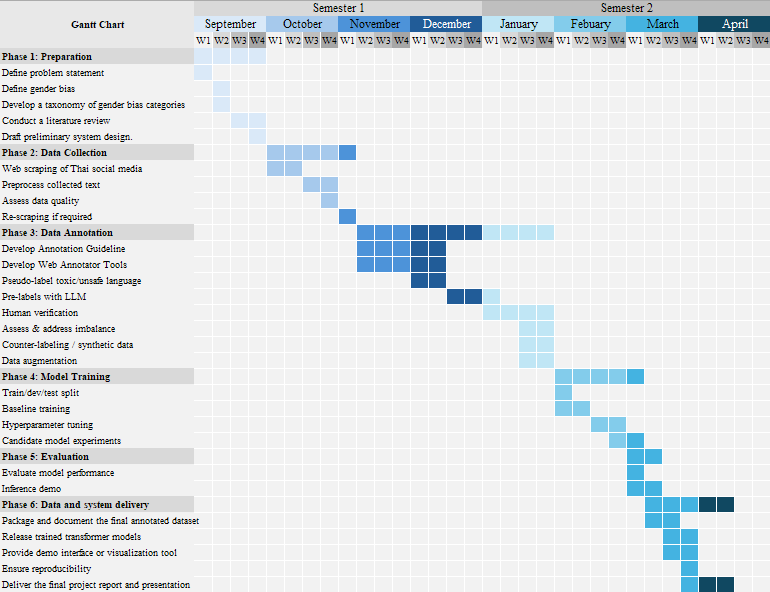
\includegraphics[width=0.8\linewidth]{assets/images/gantt_chart.png}
\caption{Gantt Chart}
\label{fig:gantt-chart}
\end{figure}

\section{Deliverables}

\subsection{Semester 1}

\begin{itemize}
\item
  {\textbf{Preliminary Report \& Design Document}\hfill\break
  Including: problem statement, related work, taxonomy, system \& dataset design, and draft annotation guidelines.}
\item
  {\textbf{Sample Dataset}\hfill\break
  A small set of Thai social media posts annotated for gender bias, with human-verified pre-labels.}
\item
  {\textbf{Prototype Baseline Setup}\hfill\break
  Initial experiment with sentence boundary heuristics and a baseline classifier for sentence-level bias detection.}
\item
  {\textbf{Annotator Tools Website}}
\end{itemize}

\subsection{Semester 2}

\begin{itemize}
\item
  {\textbf{Final Annotated Dataset}}
  \begin{itemize}
  \item
    {Complete dataset with tokens, rationales, triggers, and sentence-level labels.}
  \item
    {Supports three tasks: sentence-level classification, span-level rationale extraction, and trigger identification.}
  \end{itemize}
\item
  {\textbf{Trained Models with Multi-Head Logits}\hfill\break
  Fine-tuned transformer models that produce:}
  \begin{itemize}
  \item
    {Sentence-level logits:~classify biased vs. non-biased sentences.}
  \item
    {Rationale logits:~token-level spans providing context for bias.}
  \item
    {Trigger logits:~token-level cues pinpointing explicit biased words.}
  \end{itemize}
\item
  {\textbf{Evaluation Results \& Error Analysis}\hfill\break
  Quantitative metrics (accuracy, F1, span-level performance) plus qualitative analysis of bias detection outputs, including rationale/trigger highlighting.}
\item
  {\textbf{Final Report}\hfill\break
  Chapters 1--5 covering methodology, experiments, results, limitations, and future work.}
\end{itemize}








\chapter{Background, Theory and Related Research}

\section{Backgrounds}

\subsection{Taxonomy Definition}

\subsubsection{Gender Bias}

According to the European Institute for Gender Equality (EIGE) \hyperlink{bib:ref9}{[9]}, gender bias refers to prejudiced actions or thoughts that arise from the perception that women are not equal to men in rights and dignity. This bias is expressed both explicitly and implicitly, and it can manifest in language, attitudes, and behaviors that reinforce unequal power relations between genders. In the context of online communication, gender bias often appears in subtle linguistic patterns that normalize inequality or perpetuate stereotypes, thereby contributing to broader systems of discrimination.

\subsubsection{Gender Stereotypes \& Role Expectations}

Gender stereotypes are preconceived ideas whereby females and males are arbitrarily assigned characteristics, abilities, and social roles that are determined and limited by their gender rather than by individual capacities \hyperlink{bib:ref10}{[10]}. ~Such stereotypes often prescribe how men and women are “expected” to behave, for example, assuming that women should be nurturing or that men should be assertive. Closely related are role expectations, which are the social and cultural pressures for individuals to act in accordance with these stereotyped roles. These expectations constrain personal freedom and reinforce inequality, as they prevent individuals from pursuing opportunities outside of what society deems “appropriate” for their gender.

\subsubsection{Sexist / Derogatory Language}

Sexism refers to actions, attitudes, or expressions that discriminate against people based solely on their gender \hyperlink{bib:ref11}{[11]}. ~In language, this can appear as derogatory expressions that diminish respect, show disapproval, or demean individuals because of their gender identity. Derogatory language may include insults, slurs, or dismissive terms that directly target gender \hyperlink{bib:ref12}{[12]}.

Within this category, two common linguistic forms are:

\begin{itemize}
\item
  {Objectification:~treating individuals as objects, tools, or commodities, reducing them to their physical attributes or perceived usefulness, as if they lack feelings, opinions, or agency \hyperlink{bib:ref13}{[13]}. }
\item
  {Sexualization:~framing or portraying a person primarily in sexual terms, often without their consent or in contexts where it is irrelevant, thereby reducing their identity to sexual desirability \hyperlink{bib:ref14}{[14]}.}
\end{itemize}

Together, these forms of sexist and derogatory language perpetuate disrespect, marginalization, and inequality in both online and offline communication.

\subsection{Theory}

\subsubsection{Transformers in Machine Learning}

The Transformer is a neural network architecture introduced in \hyperlink{bib:ref26}{[26]} that has become the foundation of modern natural language processing. Unlike recurrent or convolutional models, Transformers rely entirely on self-attention mechanisms to model relationships between tokens, allowing them to process sequences in parallel and capture long-range dependencies efficiently \hyperlink{bib:ref15}{[15]}.

A Transformer consists of two main components:

\begin{itemize}
\item
  {\textbf{Encoder}: processes the input sequence and generates contextualized representations.}
\item
  {\textbf{Decoder}: generates the output sequence step by step, attending to both the encoder outputs and previously generated tokens.}
\end{itemize}

Key innovations of the Transformer include:

\begin{itemize}
\item
  {\textbf{Multi-head self-attention}: enables the model to learn different types of dependencies in parallel.}
\item
  {\textbf{Positional encoding}: provides information about the order of tokens, compensating for the lack of recurrence.}
\item
  {\textbf{Layer normalization and residual connections}: stabilize training and improve gradient flow.}
\end{itemize}

Transformers achieve state-of-the-art performance on machine translation tasks and have since become the backbone of large-scale pretrained models such as BERT, GPT, RoBERTa, and XLM-R. These models enable applications beyond translation, including sentence-level classification, span detection, summarization, and text generation.

The architecture's flexibility, scalability, and parallelism make Transformers particularly powerful for tasks involving long, unstructured, or noisy text, which are central to social media analysis and gender bias detection.

\subsubsection{Multi-Head Attention Mechanism}

The multi-head attention mechanism is a central component of Transformer models, enabling them to capture different types of relationships between tokens in parallel \hyperlink{bib:ref16}{[16]}. Unlike traditional attention, which produces a single weighted representation of input tokens, multi-head attention projects the input into multiple subspaces and computes attention separately in each.

Formally, each head performs the scaled dot-product attention:

\[\text{Attention}(Q, K, V) = \text{softmax}\left(\frac{QK^T}{\sqrt{d_k}}\right)V\]

where Q(queries), K(keys), and V(values) are linear projections of the input embeddings, and dkd\_kdk is the dimension of the key vectors.

By using multiple attention heads, the model can:

\begin{itemize}
\item
  {Focus on different types of dependencies (e.g., syntactic, semantic, positional).}
\item
  {Capture short-range and long-range interactions simultaneously.}
\item
  {Provide richer contextual representations than single-head attention.}
\end{itemize}

The outputs from all heads are concatenated and linearly projected to form the final representation. This design allows the model to integrate multiple perspectives, improving both expressiveness and interpretability.

\subsubsection{Classifiers in Machine Learning}

In machine learning, a classifier is an algorithm that maps input data into predefined categories or classes \hyperlink{bib:ref17}{[17]},\hyperlink{bib:ref18}{[18]}. Classifiers form the basis of supervised learning, where models are trained on labeled data to learn decision boundaries that separate one class from another. They are widely used in tasks such as spam detection, sentiment analysis, medical diagnosis, and bias detection.

Common types of classifiers include:

\begin{enumerate}
\item
  {\textbf{Logistic Regression}: A statistical model that predicts the probability of a class label using a logistic (sigmoid) function. It is simple, interpretable, and effective for linearly separable data.}
\item
  {\textbf{Naïve Bayes Classifier}: A probabilistic model based on Bayes' theorem with the assumption of feature independence. It is computationally efficient and often used for text classification.}
\item
  {\textbf{K-Nearest Neighbors (KNN)}: An instance-based method that assigns a label to new data based on the majority class of its nearest neighbors in the feature space. It is intuitive but computationally expensive at prediction time.}
\item
  {\textbf{Support Vector Machines (SVM)}: A margin-based classifier that finds the optimal hyperplane separating classes. It is powerful for both linear and non-linear decision boundaries through kernel functions.}
\item
  {\textbf{Decision Trees}: Models that split data recursively based on feature values to form a tree structure of decisions. They are interpretable and handle non-linear relationships well but can overfit.}
\item
  {\textbf{Ensemble Methods (e.g., Random Forest, Gradient Boosting)}: Combine multiple classifiers to improve robustness and accuracy. They reduce variance and bias compared to single models and are widely used in practice.}
\end{enumerate}

\subsubsection{Topic Coherence and Topic Diversity}

Topic coherence \hyperlink{bib:ref19}{[19]} is a fundamental evaluation metric in topic modeling, measuring how semantically interpretable and meaningful the discovered topics are. A coherent topic is one in which the top words frequently co-occur in similar contexts and form a concept that humans can readily understand. Because BERTopic and related embedding-based clustering methods do not rely on traditional probabilistic topic-word distributions, coherence offers an essential way to validate the quality of generated clusters.

Coherence scores formalize semantic similarity among top-ranked topic words using statistical or embedding-based measures. One of the most widely adopted metrics is $c_v$~coherence, which relies on normalized pointwise mutual information (NPMI) and cosine similarity in a sliding-window context space. Formally, the NPMI between two words $w_i$~and $w_j$~is:

\[\text{NPMI}(w_i, w_j) = \frac{\log \frac{P(w_i, w_j)}{P(w_i)P(w_j)}}{-\log P(w_i, w_j)}.\]

The coherence of a topic consisting of words $\{w_1, w_2, \dots, w_k\}$~is computed as the average pairwise NPMI similarity:

\[\text{Coherence}_{c_v}(T) = \frac{1}{\binom{k}{2}} \sum_{i < j} \text{NPMI}(w_i, w_j)\]

High coherence indicates that topic words capture a consistent semantic theme, while low coherence signals noisy or uninterpretable clusters.

While coherence evaluates internal consistency, topic diversity measures whether topics are distinct from one another. A topic model with high coherence but low diversity may simply repeat the same vocabulary across multiple clusters. Topic diversity is typically computed as:

\[\text{Diversity} = \frac{|\text{Unique Topic Words}|}{|\text{Total Topic Words}|}\]

A balanced topic model should exhibit both high coherence (quality) and high diversity (coverage).

\subsubsection{Evaluation Metrics for Classification}

Evaluation metrics are used to measure how well a machine learning model performs on a given task. In classification problems, common metrics include accuracy, precision, recall, and F1-score. These metrics help evaluate different aspects of model performance, especially when the dataset is imbalanced and accuracy alone may not fully represent how well the model performs across all classes \hyperlink{bib:ref20}{[20]}.

Accuracy measures the proportion of correct predictions among all predictions. It provides an overall view of model performance, but it may be misleading when one class appears much more frequently than another. For example, in an imbalanced dataset, a model may achieve high accuracy by mostly predicting the majority class.

\[\text{Accuracy} = \frac{TP + TN}{TP + TN + FP + FN}\]

Precision measures how many samples predicted as positive are actually correct. In this project, precision helps evaluate whether the model incorrectly classifies NON-GB sentences as GB. A high precision score means that when the model predicts gender bias, the prediction is likely to be correct.

\[\text{Precision} = \frac{TP}{TP + FP}\]

where TP = True Positives, FP = False Positives.

Recall measures how many actual positive samples are correctly detected by the model. For gender-bias detection, recall is important because it shows whether the model can successfully identify sentences that truly contain gender bias. A low recall score means that many biased sentences are missed by the model.

\[\text{Recall} = \frac{TP}{TP + FN}\]

where FN = False Negatives.

F1-score combines precision and recall into a single metric using their harmonic mean. It is useful when both false positives and false negatives are important. In this project, F1-score is especially useful for evaluating GB and NON-GB classification as well as GB subtype classification, where class imbalance may affect model performance.

\[F_1 = 2 \cdot \frac{\text{Precision} \cdot \text{Recall}}{\text{Precision} + \text{Recall}}\]

\subsubsection{Sequence Labeling and BIO Tagging}

Sequence labeling is a natural language processing task in which each token in a sentence is assigned a label. This approach is commonly used in tasks such as named entity recognition and span detection, where the goal is to identify specific words or phrases within a text. In this project, span-level gender-bias detection can be treated as a sequence labeling task because the model must identify which tokens belong to rationale or trigger spans.

BIO tagging is a common format for representing token-level spans in sequence labeling. The BIO scheme uses three labels: B, I, and O. B marks the beginning of a span, I marks tokens inside or continuing the same span, and O marks tokens outside any span. This structure allows multi-token spans to be represented clearly and makes it possible to distinguish where a biased phrase starts, continues, and ends. BIO tagging is especially useful because assigning only a general label to each token can create ambiguity when multiple spans appear close together or when a span contains several tokens \hyperlink{bib:ref21}{[21]}.

For example, in a gender-bias sentence, a trigger phrase may consist of more than one token. Using BIO tagging, the first token of the trigger can be labeled as B-TRIGGER, the following tokens as I-TRIGGER, and all unrelated tokens as O. Similarly, rationale spans can be encoded using labels such as B-RATIONALE~and I-RATIONALE. This format makes the annotation suitable for training token-level models and evaluating whether the model can correctly identify biased expressions within a sentence.

However, BIO tagging also introduces class imbalance at the token level because most tokens in a sentence are usually labeled as O, while only a smaller number belong to rationale or trigger spans. This imbalance must be considered during model training and evaluation, since a model that predicts mostly O labels may appear accurate but fail to detect meaningful biased spans.

\subsubsection{XML-Style Tagging for Structured Prompting}

XML-style tagging is a prompt-structuring technique that uses paired tags, such as \texttt{<instruction>}\ldots\texttt{</instruction>} or \texttt{<input>}\ldots\texttt{</input>}, to separate different parts of a prompt. In large language model applications, these tags help distinguish between instructions, context, input data, examples, and expected output format. This reduces ambiguity because the model can interpret each section according to its role rather than treating the entire prompt as one continuous block of text \hyperlink{bib:ref22}{[22]}.

In span-level detection tasks, XML-style tags can also be used as an inline annotation format. For example, a model may be instructed to reproduce the input text while wrapping biased spans with labels such as \textless GB-NORMATIVE\textgreater...\textless/GB-NORMATIVE\textgreater, \textless GB-ATTACK\textgreater...\textless/GB-ATTACK\textgreater, or \textless GB-SEX\textgreater...\textless/GB-SEX\textgreater. This format is intuitive because it directly marks the location of biased spans inside the original text. It also makes the output readable for humans and similar to how span annotations are visually highlighted in annotation tools.


However, XML-style tagging has limitations when used with generative models. Since the model generates free-form text, it may produce malformed tags, add explanations outside the required format, or fail to close tags correctly. User input may also contain characters such as \textless, \textgreater, or \&, which can interfere with tag structure if not properly sanitized. Therefore, XML-style tagging is useful for structuring prompts and demonstrating span boundaries, but it may require strict formatting rules, input cleaning, and output validation before being used in an automated extraction pipeline. For this reason, structured JSON output may be preferred when machine-readable consistency is more important than inline readability.

\subsubsection{Structured JSON Output for LLM-Based Extraction}

Structured JSON output is a method for constraining a large language model to return information in a predefined machine-readable format. Instead of allowing the model to generate free-form text, the expected output is defined using a fixed structure, such as a JSON object with specific keys and value types. This is useful in information extraction tasks because the output can be automatically parsed, validated, and passed into downstream systems without requiring manual cleanup. OpenAI's structured output documentation describes this approach as a way to ensure that model responses follow a supplied JSON Schema, making outputs more reliable for application pipelines \hyperlink{bib:ref23}{[23]}.

In this project, structured JSON output is relevant to span-level gender-bias detection because the model must return extracted bias spans in a consistent format. For example, instead of generating an explanation or rewriting the sentence, the model can be instructed to output a JSON object with fixed keys such as GB-NORMATIVE, GB-SEX, and GB-ATTACK, where each key maps to a list of span strings copied from the input. This format reduces ambiguity and makes the output easier to evaluate against human-annotated spans.

Compared with free-form or XML-style inline tagging, structured JSON output provides stronger control over the expected response format. Free-form generation may include extra explanations, malformed tags, or inconsistent formatting, while JSON-based output can be checked using a parser such as json.loads(). Research and technical discussions on structured output generation also highlight the use of JSON Schema and grammar-based decoding to improve the reliability of LLM outputs, especially when outputs are consumed directly by software systems \hyperlink{bib:ref24}{[24]}.

However, structured JSON output does not guarantee that the extracted content is semantically correct. A model may produce valid JSON while still selecting the wrong span or assigning the wrong label. Therefore, JSON structure mainly improves format consistency and downstream usability, while extraction quality must still be evaluated using span-level metrics such as token-level precision, recall, and F1-score.

\subsubsection{Parameter-Efficient Fine-Tuning with LoRA}

Parameter-efficient fine-tuning is a method for adapting a pretrained large language model to a specific task without updating all of its original parameters. One common technique is Low-Rank Adaptation (LoRA), which keeps the base model weights frozen and inserts small trainable adapter matrices into selected model layers. Instead of fine-tuning the full weight matrix, LoRA learns two smaller low-rank matrices that approximate the required update. This greatly reduces the number of trainable parameters and lowers the memory and computational cost of fine-tuning \hyperlink{bib:ref25}{[25]}.

LoRA is useful when working with large language models because full fine-tuning can be expensive, slow, and difficult to run on limited hardware. By training only the adapter parameters, LoRA makes it possible to adapt a model using fewer GPU resources while still preserving most of the knowledge stored in the original pretrained model. During inference, the learned adapter weights are combined with the base model weights to produce task-specific outputs \hyperlink{bib:ref26}{[26]}.

In this project, LoRA is relevant to span-level gender-bias detection because the span extraction task requires the model to follow a specific annotation format and identify biased expressions from Thai social media text. Since the amount of human-annotated span-level data is limited, LoRA provides a practical way to adapt a generative model without requiring full model retraining. Important LoRA configuration choices include the rank value, which controls the size of the low-rank update, and the target modules, which determine which parts of the transformer model receive adapter layers. These choices affect both training cost and model quality \hyperlink{bib:ref27}{[27]}.

LoRA can also be combined with quantization in QLoRA, where the base model is loaded in low-bit precision while adapter parameters are trained. This further reduces GPU memory usage and makes fine-tuning more practical for resource-constrained environments. However, LoRA does not automatically guarantee better extraction quality; the model still requires well-designed training data, clear output formatting, and careful evaluation to ensure that the generated spans match the annotation guideline.

\subsubsection{Multilingual Benchmarking}

Multilingual benchmarking is used to evaluate whether a language model can perform reliably across different languages and subject domains. One commonly used benchmark is MMLU, or Massive Multitask Language Understanding, which evaluates large language models using multiple-choice questions across a wide range of subjects. MMLU covers 57 subjects, including mathematics, history, law, computer science, and ethics, making it useful for assessing both knowledge coverage and reasoning ability \hyperlink{bib:ref28}{[28]}.

In multilingual model selection, MMLU and its multilingual variants are useful because they provide a standardized way to compare models beyond a single task or language. A model with stronger multilingual benchmark performance is generally more suitable for tasks involving low-resource or non-English text, such as Thai social media analysis. However, MMLU scores should not be treated as a direct measure of gender-bias detection performance, because the benchmark mainly tests general knowledge and reasoning through multiple-choice questions rather than social bias detection or span extraction.

DeepEval provides an implementation framework for evaluating LLMs on benchmarks such as MMLU. It describes MMLU as a benchmark based on multiple-choice questions across 57 subjects and highlights its usefulness for identifying areas where a model may lack understanding in specific topics \hyperlink{bib:ref29}{[29]}. In this project, multilingual benchmark results are used only as supporting evidence when considering the general language and reasoning capability of candidate models. Final model quality must still be evaluated using project-specific metrics, such as GB/NON-GB classification performance and span-level overlap with human annotations.

\section{Related Work}

\subsection{Hate Speech Detection in Thai Social Media with Ordinal-Imbalanced Text Classification}

Pasupa and Karnbanjob \hyperlink{bib:ref30}{[30]} address the problem of hate speech detection in Thai social media by constructing a labeled dataset and benchmarking multiple deep learning models, including CNN, LSTM, BiLSTM, BiGRU, and hybrid CNN--LSTM architectures. Their study emphasizes the importance of preprocessing steps such as Thai word segmentation and the use of distributed word embeddings (Word2Vec, FastText) tailored to the Thai language. The experimental results show that recurrent and hybrid sequence models achieve higher performance compared to shallow baselines, highlighting the suitability of sequence-based architectures for noisy, user-generated content. Although the target phenomenon differs, the methodological insights are directly applicable to gender bias detection: both tasks involve identifying socially sensitive linguistic phenomena in informal Thai texts. In particular, their findings motivate the use of Thai-specific preprocessing, embedding selection, and sequence modeling as critical design choices for building robust span- and sentence-level bias detectors.

\subsection{Situated Data, Situated Systems: A Methodology to Engage with Power Relations in Natural Language Processing Research}

Lucy et al. \hyperlink{bib:ref31}{[31]} argue for a situated methodology in natural language processing research, emphasizing that data and systems are embedded within social and power relations. They propose a framework that highlights the importance of examining who creates datasets, how annotation guidelines reflect social assumptions, and whose perspectives are prioritized or marginalized. While the paper does not present computational models, it contributes a methodological lens for designing and documenting datasets and systems in socially sensitive domains such as bias detection. For our project, this perspective underscores the need to treat bias annotation and rationale labeling as situated practices, where annotator guidelines and interpretive frameworks shape the outcomes of automated systems. Accordingly, their work informs the data methodology and ethical positioning of our study, complementing technical advances in span-level bias detection with a recognition of the broader social dynamics involved.

\subsection{HateXplain: A Benchmark Dataset for Explainable Hate Speech Detection*}

Mathew et al. \hyperlink{bib:ref32}{[32]} introduce HateXplain, a benchmark dataset for explainable hate speech detection, in which annotators not only label text for hate and offensiveness but also highlight rationales and identify target communities. This dataset enables models to be evaluated not only on classification accuracy but also on their ability to produce explanations that align with human annotations. Experiments with transformer-based models such as BERT, RoBERTa, and XLNet show that while classification performance is strong, models struggle to replicate human-provided rationales, underscoring the difficulty of aligning machine explanations with human judgments. For our project, HateXplain is especially relevant as it provides a methodological precedent for trigger--rationale annotation schemes and for evaluating models by comparing their explanatory spans to human annotations. This directly supports our span-level bias detection framework, where explanation and interpretability are central to the system's value.

\subsection{Gender Bias in Coreference Resolution: Evaluation and Debiasing Methods}

Zhao et al. \hyperlink{bib:ref33}{[33]} examine gender bias in coreference resolution systems and propose both evaluation and debiasing strategies. They introduce the WinoBias dataset, a set of controlled Winograd-style sentence pairs designed to test whether models disproportionately link occupational roles with stereotypical genders. Their analysis reveals that state-of-the-art systems display strong gender associations, resolving coreference in biased ways. To address this, they implement two debiasing techniques: data augmentation through gender swapping and embedding debiasing via vector neutralization. Both approaches significantly reduce gender bias while maintaining competitive performance on standard benchmarks. This study is directly relevant to our work in two ways: first, it illustrates how bias can be formally operationalized and tested in NLP models, and second, it offers concrete debiasing strategies such as data augmentation and embedding balancing that can inform mitigation in gender bias detection systems for Thai social media.

\subsection{Hybrid Annotation for Propaganda Detection: Integrating LLM Pre-Annotations with Human Intelligence}

Sahitaj et al. \hyperlink{bib:ref34}{[34]} introduce a hybrid annotation methodology for propaganda detection that leverages large language models (LLMs) to generate pre-annotations subsequently validated by human annotators. Their study demonstrates that such hybrid workflows significantly reduce annotation time and cognitive effort while preserving, and in some cases improving, the quality of the resulting dataset compared to fully manual annotation. The authors further show that models trained on hybrid-annotated data achieve competitive performance, confirming the practical utility of this approach. Importantly, they note that LLM pre-annotations contain systematic errors that necessitate human oversight, especially in nuanced or context-dependent cases. For our project, this work provides a methodological precedent for using LLM-assisted pre-labeling with human correction in building a gender bias dataset, enabling efficient span- and rationale-level annotation without compromising data integrity.

\subsection{Syllable-based Neural Thai Word Segmentation}

Chormai et al. \hyperlink{bib:ref35}{[35]} address the challenge of Thai word segmentation, a prerequisite for most downstream NLP tasks, by proposing a syllable-based neural segmentation model. Unlike character-based or dictionary-driven methods, their approach leverages syllables as intermediate units and employs neural sequence models, including BiLSTM--CRF and Transformer-based encoders. Experimental results show that syllable-based segmentation not only surpasses traditional methods in accuracy but also improves the performance of downstream applications such as part-of-speech tagging and dependency parsing. Importantly, the model demonstrates robustness on informal and noisy text, making it particularly suitable for social media contexts. For our project, this work provides a methodological foundation for preprocessing: effective segmentation is essential for span-level gender bias detection in Thai, and adopting a syllable-based approach can reduce tokenization errors that might otherwise obscure or distort biased expressions.

\subsection{Attention Is All You Need}

Vaswani et al. \hyperlink{bib:ref36}{[36]} revolutionized sequence modeling by introducing the Transformer architecture, which relies exclusively on self-attention mechanisms to capture dependencies between tokens. The Transformer eliminates recurrence and convolution, replacing them with multi-head self-attention and positional encodings within an encoder--decoder framework. A central innovation of this design is that multi-head attention enables the model to capture diverse relational patterns in parallel, allowing different heads to focus on distinct aspects of linguistic structure. This architecture achieves highly parallelizable training and state-of-the-art performance on large-scale translation benchmarks, while modeling long-range contextual dependencies more effectively than RNN- or CNN-based models. As the foundation of modern natural language processing, Transformer-based models such as BERT, RoBERTa, and XLM-R have enabled both sentence-level classification and fine-grained span detection tasks.

Building on this foundation, recent work has shown that multi-head attention can be enriched with constraints, such as syntax- or discourse-aware masking, to enhance interpretability and robustness. Inspired by this line of research, our project adapts the concept of specialized attention streams by producing three distinct sets of logits: (i) sentence-level logits for global classification of bias, (ii) rationale logits for span-level evidence supporting the classification, and (iii) trigger logits for token-level cues pinpointing biased expressions. By explicitly separating these outputs, our model is able to improve both accuracy and interpretability, allowing the system to justify its predictions through span highlights in line with the broader trend toward explainable NLP.

\subsection{Syntax-Based Attention Masking for Neural Machine Translation}

McDonald and Chiang \hyperlink{bib:ref37}{[37]} proposed Syntax-Based Attention Masking, which augments multi-head attention with syntactic tree constraints. Each attention head can dynamically learn to attend to parent, child, or sibling nodes in a parse tree, rather than relying solely on linear token order. Their method consistently improved machine translation accuracy for low-resource languages by up to +2.1 BLEU. The insight here is that different heads can specialize in structural relationships, analogous to how our model separates rationale heads (capturing supportive spans) from trigger heads(identifying explicit biased expressions).

\subsection{Long-Short Term Masking Transformer: A Simple but Effective Baseline for Document-level Neural Machine Translation}

Zhang et al. \hyperlink{bib:ref38}{[38]} introduced the Long-Short Term Masking Transformer, which maintains two parallel streams of attention: a global stream that captures cross-sentence context and a local stream restricted to the current sentence. This design reduces error propagation across sentences while preserving discourse consistency. Their experiments in document-level machine translation showed that such masking strategies improve both BLEU scores and coherence in longer texts . This highlights how tailored attention heads can manage different granularities of context, a principle directly relevant to our span- and sentence-level gender bias detection, where both local cues (biased words) and global cues (overall tone of the post) must be integrated.

\subsection{Semi-supervised Thai sentence segmentation using local and distant word representations}

Saetia et al. \hyperlink{bib:ref39}{[39]} present a semi-supervised approach to Thai sentence segmentation that integrates local and distant word representations. Their model combines n-gram-based local embeddings with self-attention mechanisms for capturing long-range dependencies, and applies cross-view training to exploit large amounts of unlabeled text alongside limited annotated data. Experimental results show that this method outperforms fully supervised baselines, particularly in resolving ambiguous sentence boundaries, and demonstrates robustness on informal Thai text. For our project, this study provides an important preprocessing foundation: reliable sentence segmentation is essential when analyzing paragraph-level social media content for bias, and the semi-supervised strategy offers a practical solution to data scarcity while mitigating segmentation errors that could compromise span-level bias detection.

\subsection{Sentence-level Media Bias Analysis Informed by Discourse Structures}

Lei et al. \hyperlink{bib:ref40}{[40]} investigate sentence-level media bias detection by incorporating discourse structures into transformer-based models. They argue that bias is not always apparent within a sentence in isolation and design models that integrate rhetorical relations and contextual cues from surrounding discourse. Experimental results show that discourse-informed models outperform BERT and RoBERTa baselines on sentence-level classification tasks, highlighting the importance of context in bias detection. For our project, this study is directly relevant as it reinforces the value of sentence-level classification as a complementary signal to span-level identification. Moreover, their discourse-informed approach parallels our own strategy of producing distinct logits for sentence, rationale, and trigger levels, ensuring that global classification is supported by localized and interpretable evidence.

\subsection{ViHOS: Hate Speech Spans Detection for Vietnamese}

Hoang et al. \hyperlink{bib:ref41}{[41]} introduce ViHOS, the first benchmark dataset for Vietnamese hate speech span detection. Each post in ViHOS is annotated at both the sentence level, indicating the presence or absence of hate speech, and the span level, identifying the exact words or phrases that constitute hate. The authors evaluate a range of sequence labeling models, including BiLSTM--CRF and transformer-based architectures such as XLM-R, showing that while transformers outperform recurrent baselines, span-level detection remains considerably more challenging than sentence classification. They further demonstrate that jointly modeling sentence- and span-level labels yields performance improvements. For our project, ViHOS is directly relevant as it exemplifies the design of dual-level annotation schemes and provides empirical support for our architecture that outputs sentence-level, rationale-level, and trigger-level logits. Moreover, as a non-English, social media--based dataset, ViHOS strengthens the case for extending span-level bias detection to Thai text.

\subsection{Heuristics-Based Detection to Improve Text/Graphics Segmentation in Complex Engineering Drawings}

Moreno-García et al. \hyperlink{bib:ref42}{[42]} investigate the problem of segmenting complex engineering drawings into text and graphics components, proposing a heuristics-based detection framework to improve accuracy. Their method leverages geometric and structural rules, such as stroke width and alignment, to distinguish between textual and graphical regions, thereby overcoming limitations of standard segmentation algorithms. The study demonstrates that heuristic rules, when informed by domain knowledge, can significantly enhance performance in cases where automated methods alone struggle. While situated in the vision domain, this work illustrates the broader methodological value of heuristic-driven approaches, supporting our decision to incorporate heuristic and fallback strategies for Thai text segmentation prior to bias detection.

\subsection{In Plain Sight: Media Bias Through the Lens of Factual Reporting}

Fan et al. \hyperlink{bib:ref43}{[43]} investigate media bias through the lens of factual reporting by constructing a dataset of news articles annotated at the sentence level for factual versus biased content. They evaluate multiple sentence encoders, including BiLSTMs, CNNs, and transformer-based models, and demonstrate that incorporating contextual information from surrounding sentences improves classification performance. Their findings highlight that bias is often expressed subtly, through lexical framing rather than overt statements, and that context is essential for reliable detection. For our project, this study provides methodological precedent for sentence-level bias detection, supporting the integration of sentence-level logits~alongside span- and trigger-level outputs. Moreover, the challenges they note in annotation reliability inform our own data design, underscoring the importance of clear guidelines and rationale labeling in socially sensitive tasks such as gender bias detection.

\subsection{Thai sentence segmentation using large language models}

Panitsrisit \hyperlink{bib:ref44}{[44]} explores Thai sentence segmentation using the LST20 corpus, which contains multilayer annotations including word boundaries, POS tags, named entities, clauses, and sentence boundaries. The corpus was preprocessed into a structured DataFrame with explicit labels: TOKENS, POS, NER, CLAUSE, and SEP, to facilitate supervised learning. While the primary contribution of this study lies in segmentation experiments, ranging from baseline Maximum Entropy classifiers to fine-tuned large language models, its methodological value extends beyond sentence boundary prediction. The DataFrame labeling scheme illustrates how raw text can be transformed into a structured sequence-labeling format, a process that parallels our own span-based bias detection task. In our project, we adopt a heuristic approach for sentence segmentation, but the idea of structuring annotated input into labeled frames directly informs our design for bias span identification, where triggers and rationales play a role similar to SEP and clause markers in segmentation.

\begin{table}[H]
\centering
\footnotesize
\caption{An example of preprocessed text in the DataFrame in \textit{Thai sentence segmentation using large language models}.}
\begin{tabularx}{\textwidth}{@{}>{\raggedright\arraybackslash}X>{\raggedright\arraybackslash}X>{\raggedright\arraybackslash}X>{\raggedright\arraybackslash}X>{\raggedright\arraybackslash}X@{}}
\toprule
\textbf{Tokens} & \textbf{POS} & \textbf{NER} & \textbf{CLAUSE} & \textbf{SEP} \\
\midrule
{}[เผย, เจ็ต, , ลี, , และ, แจ็กกี้, , ชำน, \ldots] & [VV, NN, PU, NN, PU, CC, NN, PU, NN, \ldots] & [O, B\_PER, I\_PER, E\_PER, O, O, B\_PER, I\_PER, E\_PER, \ldots] & [B\_CLS, I\_CLS, I\_CLS, E\_CLS, O, B\_CLS, I\_CLS, \ldots] & [N, N, N, N, N, N, N, N, N, \ldots] \\
{}[เป็น, หนัง, แอ็กชั่น, ที่, มี, ฉำก, แสดง, \ldots] & [NN, NN, NN, VV, AX, NN, \ldots] & [O, O, O, O, O, O, \ldots] & [B\_CLS, I\_CLS, E\_CLS, \ldots] & [N, N, N, N, N, N, \ldots] \\
{}[นำยก, รัฐมนตรี, ญี่ปุ่น, เรียกร้อง, ให้, จีน, \ldots] & [NN, NN, NN, NN, NN, VV, NN, \ldots] & [O, O, B\_LOC, O, O, B\_LOC, \ldots] & [B\_CLS, I\_CLS, I\_CLS, I\_CLS, I\_CLS, \ldots] & [N, N, N, N, N, \ldots] \\
{}[สำว, ม., ปลำย, สำธำรณรัฐ, เช็ก, คว้ำ, มงกุฎ, \ldots] & [VV, NN, NN, CC, VV, NN, VV, \ldots] & [O, O, O, O, O, O, \ldots] & [B\_CLS, I\_CLS, I\_CLS, I\_CLS, I\_CLS, \ldots] & [N, N, N, N, N, N, \ldots] \\
\bottomrule
\end{tabularx}
\end{table}

\subsection{An Annotated Corpus for Sexism Detection in French Tweets}

Chiril et al. \hyperlink{bib:ref45}{[45]} introduce the first annotated corpus for sexism detection in French tweets, comprising approximately 12,000 annotated instances sampled from 115,000 tweets collected between 2017 and 2018. Their annotation scheme, grounded in speech act theory, distinguishes three categories: (i) direct sexist assertions, addressed to women; (ii) descriptive sexist assertions, referring to women in general; and (iii) reported assertions, which recount or denounce instances of sexism. Importantly, the latter category is not considered abusive content for moderation purposes, representing a key methodological contribution that aligns dataset design with practical considerations for content moderation. Annotation reliability is strong, with Cohen's $\kappa$ values between 0.71 and 0.72. The authors benchmark several models, ranging from SVMs with bag-of-words features to deep architectures such as CNNs, CNN--LSTM hybrids, BiLSTM with attention, and multilingual BERT (mBERT). Among these, mBERT achieves the best performance (accuracy of 0.79; macro-F1 of 0.762). Error analysis highlights challenges in detecting irony and satire, benevolent sexism, stereotypical framings, and tweets requiring pragmatic inference due to emojis, URLs, or other context-dependent cues.

For our project, this work is instructive in two respects. First, we adopt their methodological distinction between direct and descriptive sexism on the one hand, and reported or denunciatory narratives on the other, in order to avoid misclassifying reportage as abusive content. To this end, our annotation guidelines mirror this taxonomy while being adapted to Thai gender norms. Second, we extend their technical contributions by incorporating multi-head outputs that produce sentence-level logits for global classification alongside span-level trigger and rationale predictions, enabling interpretable detection that identifies the specific tokens encoding bias. Furthermore, we address limitations observed in their corpus by preserving pragmatic cues common in short posts---for example, by expanding emojis and substituting URL titles, so that context is retained for models to disambiguate ironic or satirical uses. Taken together, this adaptation yields a moderation-aware and interpretable pipeline tailored to Thai social media and blogs: an annotation design that respects reportage, preprocessing that preserves pragmatic signals, and modeling that not only flags biased content but also explains its linguistic basis at the word or phrase level.

\subsection{BennettNLP at SemEval-2021 Task 5: Toxic Spans Detection using Stacked Embedding Powered Toxic Entity Recognizer}

Kataria et al. \hyperlink{bib:ref46}{[46]} present BennettNLP, a system for the SemEval-2021 Toxic Spans Detection task that reframes toxicity identification as a sequence-labeling / NER problem. The authors propose a stacked-embedding architecture implemented in the flairNLP framework, combining contextual Flair embeddings, BERT (base/large, uncased), character embeddings, and optionally GloVe, followed by a BiLSTM-CRF decoding layer to predict token-level toxic spans. A key contribution is their linked-list--based preprocessing pipeline, which cleans noisy social media text (punctuation, numerals, foreign characters) while preserving character indices so that gold spans remain aligned after normalization. Evaluated on Civil Comments--derived data, their best configuration achieves an F1 score of 0.748, outperforming other published systems on the shared task. For our project, BennettNLP is directly relevant as it demonstrates how toxic content can be modeled at span level with NER-style architectures and careful span-preserving preprocessing. We draw on this work both conceptually, treating gender-bias markers as “toxic entities” requiring span annotations, and practically, by using BennettNLP-style toxic span detection as an upstream pseudo-labeling signal to prioritize candidate sentences for our own trigger--rationale gender bias annotation pipeline.

\subsection{CREST: Universal Safety Guardrails Through Cluster-Guided Cross-Lingual Transfer}

Bansal and Mishra \hyperlink{bib:ref47}{[47]} introduce CREST (CRoss-lingual Efficient Safety Transfer), a multilingual safety classification model designed to address the limitations of existing guardrails that mainly focus on high-resource languages such as English, Chinese, and Spanish. CREST supports 100 languages using only 0.5B parameters, making it substantially lighter than typical LLM-based safety models while still achieving competitive or superior performance.

The key innovation of CREST lies in its cluster-guided cross-lingual transfer approach. Instead of training on all target languages, which is infeasible for low-resource languages lacking labeled datasets, CREST identifies structural and representational similarities between languages using XLM-R embeddings. Languages are grouped into clusters, and the system is trained only on 13 strategically chosen high-resource languages, one or two from each cluster. This enables effective zero-shot generalization to both high-resource and low-resource languages within the same cluster. The model demonstrates strong transfer capabilities on over 100 languages, including Thai, even though many of these languages were not part of the training set.

CREST is evaluated across multiple multilingual safety benchmarks (Aegis-CS2, HarmBench, RTP-LX, Polyglot Toxicity Prompts) and consistently outperforms other lightweight guardrails, achieving performance comparable to or better than larger models ($\geq$2.5B parameters). The model also shows robustness on culturally nuanced datasets and code-switching scenarios, an important property for real-world social media environments.

For the present study, CREST is relevant in two major ways. First, it provides a reliable pseudo-labeling layer for filtering general unsafe or toxic content prior to gender-bias annotation, reducing the burden on downstream LLM pre-labeling and human reviewers. Second, its effectiveness in low-resource languages supports the feasibility of applying safety-aligned filtering in Thai, where high-quality safety datasets are limited. CREST therefore strengthens the preprocessing pipeline by ensuring that only contextually appropriate, non-harmful, and relevant samples are passed into the gender-bias detection workflow.




\chapter{Methodology and Design}

\section{Methodology Overview}

\begin{figure}[H]
\centering
\includegraphics[width=0.9\linewidth]{assets/images/overview.png}
\caption{Methodology Overview}
\label{fig:methodology-overview}
\end{figure}




Figure~\ref{fig:methodology-overview} summarizes the methodology of this project, which consists of five main stages: data collection, data annotation, synthetic data generation, model training, and evaluation. First, Thai social media data are collected from TikTok, Twitter/X, and YouTube using platform-specific scraping methods. The extracted content is then cleaned, preprocessed, and explored through exploratory data analysis (EDA). In this stage, topic modeling is used to examine the thematic structure of the corpus and identify topic groups that are more likely to contain gender- and SOGI-related expressions.

After data collection and preprocessing, the next stage is data annotation. An annotation guideline is designed to define the label structure, decision rules, and span-selection criteria for gender-bias detection. A web-based annotator tool is then used to support human annotators in labeling the dataset. The annotation process produces sentence-level labels, GB subtypes, decision rules, rationale spans, and trigger spans, which serve as the human-annotated ground truth for evaluation and future model improvement.

To address data imbalance and increase the diversity of training examples, synthetic data generation is applied. Gemini 2.5 Flash is used to generate Thai social-media-style examples based on the project's annotation taxonomy. The synthetic data provide balanced examples across GB-ATTACK, GB-NORMATIVE, GB-SEX, neutral, meta\_counter, and gendered\_insult classes, allowing the sentence-level model to learn the overall label structure before being evaluated on real annotated data.

The model training stage consists of two main tasks: sentence-level classification and span-level extraction. The sentence-level model predicts whether a given sentence contains gender bias and, when applicable, identifies the GB subtype. The span-level model extracts biased text spans grouped by GB subtype using a structured JSON output format. Although the human annotation scheme includes both rationale and trigger spans, the current span-level model does not yet predict them separately.

Finally, the trained models are evaluated using human-annotated data. Sentence-level evaluation uses accuracy, precision, recall, F1-score, and AUC-ROC to measure binary GB/NON-GB classification and GB subtype classification. Span-level evaluation compares extracted GB spans with human-annotated biased spans using exact-match span F1, character-level F1, and faithfulness rate. Error analysis is then conducted to identify common issues such as overprediction, stance sensitivity, subtype confusion, boundary mismatch, and context-dependent bias.

\section{Data Collection}

Following the pipeline in Section 3.1, we began with large-scale data collection from Thai social media. In this phase, we focused on three platforms, Twitter/X, YouTube, and TikTok.

To support multi-platform data collection, we implemented different scraping methods based on the technical limitations of each platform. Because each social media service exposes its content in distinct ways, the project uses a combination of Selenium automation, official/unofficial APIs, and metadata parsers.

\subsection{Twitter/X Data Collection}

Twitter/X data were collected using a Selenium-based scraping method. Selenium was used because Twitter/X pages load content dynamically, meaning that tweets, replies, and quoted posts are often loaded only after scrolling or interacting with the page. By controlling a real Chrome browser session, Selenium allows the scraper to access visible page content, maintain login status, scroll automatically, and extract tweet elements in a way that resembles normal user browsing.

The Twitter/X data collection process followed these steps:

\begin{enumerate}
\item
  {\textbf{Open Chrome with a persistent user profile}\\
  \strut ~~~~~~~~The scraper opens Google Chrome using a saved browser profile. This keeps the login session, cookies, and browser settings active across scraping runs. This is important because Twitter/X often limits content visibility for users who are not logged in.}
\item
  {\textbf{Load the target Twitter/X page}\\
  \strut ~~~~~~~~The scraper loads a selected target page, such as a tweet page, user timeline, search result page, or reply thread. These pages are used to collect different types of content, including original tweets, replies, and quoted posts.}
\item
  {\textbf{Automatically scroll through the page}\\
  \strut ~~~~~~~~Since Twitter/X uses dynamic loading, not all content appears at once. The scraper scrolls through the page automatically to trigger the loading of more tweets and replies.}
\item
  {\textbf{Detect tweet elements on the page}\\
  \strut ~~~~~~~~As new content appears, Selenium identifies tweet containers and related HTML elements. This allows the scraper to locate each tweet or reply separately before extracting its information.}
\item
  {\textbf{Extract text and metadata}\\
  \strut ~~~~~~~~For each detected tweet, the scraper extracts the main text, timestamp, tweet ID or URL when available, and engagement information such as likes, reposts, replies, or views. These fields help preserve both the content and useful contextual information.}
\item
  {\textbf{Remove duplicate records}\\
  \strut ~~~~~~~~Because the same tweet may appear multiple times during scrolling or across different pages, duplicate records are removed. This prevents repeated content from affecting later analysis and model training.}
\item
  {\textbf{Save the extracted data into CSV format}\\
  ~~~~~~~~The final extracted records are stored as structured CSV files. This format allows the Twitter/X data to be combined with data from other platforms and used in later stages such as preprocessing, exploratory data analysis, annotation, and model training.}
\end{enumerate}

\subsection{TikTok Data Collection}

TikTok data were collected using the TikTokApi library. This method was selected because TikTok content, especially comments, is difficult to collect through simple static page scraping. TikTokApi allows the scraper to create a browser-based session, access public video data, and retrieve comments from specific target video IDs. Since TikTok comments are usually short, informal, and reactive, they are useful for capturing casual expressions, slang, teasing, and emotionally driven responses that may contain gender-related language.

The TikTok data collection process followed these steps:

\begin{enumerate}
\item
  {\textbf{Create a TikTokApi browser session}\\
  ~~~~~~~~The scraper first creates a browser session using TikTokApi. A valid session token is required to access TikTok content more reliably and reduce access restrictions during scraping.}
\item
  {\textbf{Specify target video IDs}\\
  ~~~~~~~~The scraper receives a list of TikTok video IDs as input. These video IDs are used as the target sources for comment extraction.}
\item
  {\textbf{Retrieve comments from each video}\\
  ~~~~~~~~For each target video, the scraper requests available comments through TikTokApi. This includes top-level comments and, when available, threaded replies.}
\item
  {\textbf{Extract comment text and metadata}\\
  ~~~~~~~~From each retrieved comment, the scraper extracts the comment text, timestamp, comment ID, and other available metadata. These fields help preserve both the content and its source information.}
\item
  {\textbf{Standardize the extracted records}\\
  ~~~~~~~~The extracted comments are converted into a consistent data format so that they can be combined with records from Twitter/X and YouTube in later stages.}
\item
  {\textbf{Remove duplicate or invalid comments}\\
  ~~~~~~~~Duplicate comments and unusable records are removed to improve dataset quality. This helps prevent repeated content from affecting later analysis, annotation, and model training.}
\item
  {\textbf{Save comments into CSV files}\\
  ~~~~~~~~The final TikTok comment records are saved as structured CSV files. These files are then used for preprocessing, exploratory data analysis, annotation, and model training.}
\end{enumerate}

\subsection{YouTube Data Collection}

YouTube data were collected using yt-dlp, a command-line tool that can extract video metadata and available public comments. This method was selected because YouTube comments are often accessible through video metadata extraction and can be exported in a structured JSON format. Compared with TikTok comments, YouTube comments are often longer and more discussion-based, making them useful for collecting opinions, arguments, social commentary, and potentially gender-biased expressions.

The YouTube data collection process followed these steps:

\begin{enumerate}
\item
  {\textbf{Select target YouTube videos}\\
  ~~~~~~~~A list of target YouTube video URLs or video IDs was prepared. These videos were selected as sources for collecting public user comments.}
\item
  {\textbf{Fetch video metadata using yt-dlp}\hfill\break
  ~~~~~~~~The scraper used yt-dlp~to retrieve metadata from each target video. Comment extraction was enabled so that available public comments could be included in the downloaded metadata.}
\item
  {\textbf{Extract comments from JSON output}\\
  ~~~~~~~~The output from yt-dlp~was saved in JSON format. The scraper then parsed this JSON file to retrieve all available comments from each video.}
\item
  {\textbf{Extract comment text and metadata}\\
  ~~~~~~~~For each comment, the scraper extracted the comment text, timestamp, comment ID, and relevant video information. These fields help preserve the source and context of each comment.}
\item
  {\textbf{Convert comments into standardized records}\\
  ~~~~~~~~The extracted comments were converted into a standardized SocialMediaRecord~format. This ensured that YouTube records followed the same structure as the Twitter/X and TikTok datasets.}
\item
  {\textbf{Remove duplicate or invalid comments}\\
  ~~~~~~~~~Duplicate comments and unusable records were removed to improve dataset quality and avoid repeated content in later stages.}
\item
  {\textbf{Export comments into CSV files}\\
  ~~~~~~~~~The final YouTube comments were exported into per-video CSV files. These files were then used for preprocessing, exploratory data analysis, annotation, and model training.}
\end{enumerate}

Despite these differences, all scraped items are normalized into a unified record format via the SocialMediaRecord~dataclass, which standardizes fields such as id, platform, platform\_type, url, content\_type, timestamp, text, raw\_text, scraper\_module, and scrape\_date, to ensure that downstream preprocessing and annotation operate on a consistent schema.

\section{Data Preprocessing}

Before conducting EDA and annotation, all scraped data underwent a preprocessing stage to standardize text quality and prepare it for later sentence segmentation and span-level annotation. The preprocessing pipeline is designed to handle informal Thai social media language, remove noise, and preserve linguistic cues relevant to gender bias detection.

\subsection{Text Cleaning}

Text cleaning was performed to standardize the scraped social media records before tokenization, annotation, and model training. Since Thai social media text often contains informal spelling, repeated characters, emojis, URLs, mentions, and inconsistent spacing, several normalization rules were applied. The goal of this step was to reduce noise while preserving meaningful linguistic cues that may be useful for detecting gender bias.

The text cleaning process consisted of the following components:

\begin{enumerate}
\item
  {\textbf{Basic text normalization}\\
  ~~~~~~~~Basic normalization was applied to remove common formatting noise from the scraped text. This included decoding HTML entities, replacing newlines and tabs, removing irregular spacing, converting multiple spaces into a single space, lowercasing English text, and normalizing Unicode sequences using pythainlp.util.normalize. URLs, mentions, and hashtags were also removed because they usually do not contribute directly to gender-bias detection.}
\item
  {\textbf{Thai-specific orthographic normalization}\\
  ~~~~~~~~Thai social media users often repeat characters, tone marks, or punctuation for emphasis. To reduce unnecessary variation, repeated Thai characters were collapsed, such as changing “ดีมากกกก” to “ดีมาก”. Repeated tone marks were also normalized, such as changing “ไง้้้้” to “ไง้”. In addition, punctuation sequences such as ellipses, repeated exclamation marks, and repeated question marks were standardized. Unwanted symbols were removed while preserving Thai characters and important punctuation.}
\item
  {\textbf{Slang and abbreviation expansion}\\
  ~~~~~~~~Common informal Thai abbreviations were expanded into their standard forms to improve consistency. For example, “ผญ” was expanded to “ผู้หญิง”, and informal variants such as “คับ”, “ค้าบ”, and “คั้บ” were normalized to “ครับ”. This step was important because gender-related abbreviations frequently appear in social media text and must be preserved in a consistent form for annotation and modeling.}
\item
  {\textbf{Laughter and expressive pattern normalization}\\
  ~~~~~~~~Repetitive laughter patterns and repeated expressive punctuation were normalized. This included standardizing sequences such as repeated laughter, ellipses, exclamation marks, and question marks. The purpose was to reduce noisy repetition while still preserving the expressive tone of the text.}
\item
  {\textbf{Floating vowel correction in Thai tokens}\\
  ~~~~~~~~Some Thai text contained isolated vowel characters caused by irregular spacing or tokenization errors. For example, “อยาก เติม า ก” was corrected to “อยาก เติม มาก”. To handle this, the text was first tokenized using PyThaiNLP's newmm tokenizer. The algorithm then detected isolated following vowels, such as “า”, “ิ”, “ี”, “ุ”, “ู”, “ะ”, and “ำ”, and merged them with the preceding consonant. Corrections were applied only to the matched span in the original string to avoid changing unrelated parts of the text.}
\item
  {\textbf{Raw text preservation}\\
  ~~~~~~~~Although cleaned text was used for preprocessing and model development, the original raw text was preserved separately. This allowed expressive markers, such as emojis and original writing style, to remain available for reference during annotation and error checking.}
\end{enumerate}

\subsection{Raw Text Preservation}

To prevent information loss, the pipeline stores two versions of each record: raw\_text and text. The raw\_text field keeps the original unmodified content from the source platform, including emojis, repeated characters, slang, and punctuation. The text field stores the cleaned version after preprocessing. This allows the cleaned text to be used for tokenization, annotation, and model training, while the original text remains available for review and error checking.

\subsection{Thai Tokenization}

After text cleaning, the cleaned text is tokenized using PyThaiNLP's newmm tokenizer. The tokenized output is stored in a new column called tokens. This column is used for span-level annotation, where rationale and trigger spans must be selected based on token indices.

\subsection{Filtering Non-Thai or Low-Content Posts}

To remove unusable records, the pipeline calculates the number of Thai characters in each text entry. Posts with fewer than five Thai characters are filtered out because they are usually emojis-only comments, spam, non-Thai text, or records with too little content for meaningful annotation and model training.

\section{Exploratory data analysis (EDA)}

Before large-scale annotation, exploratory data analysis (EDA) was conducted to examine the collected social media corpus. The purpose of this stage was to understand the dataset's content, thematic structure, and distribution across platforms. EDA helped identify dominant topics, discover clusters likely to contain gender- and SOGI-related expressions, and refine the annotation guideline based on actual social media language rather than only theoretical definitions.

The EDA process was implemented using a Python-based clustering service. This service supports two complementary topic modeling approaches: a lightweight LDA-based model without sentence embeddings and a BERTopic-based model using Thai-compatible sentence embeddings. Both approaches share the same preprocessing layer to ensure consistency across experiments. The pipeline also provides command-line and programmatic interfaces, making the analysis reproducible and easier to rerun with different configurations.

\subsection{Preprocessing for Topic Modeling}

Before applying LDA and BERTopic, the text was processed using the standardized Thai preprocessing pipeline described in the data preprocessing section. After cleaning and tokenization, the remaining tokens were joined into a whitespace-separated string. This format makes the text suitable for vectorizers used in LDA and for embedding-based topic modeling in BERTopic, while keeping the preprocessing consistent across both methods.

\subsection{Topic Modeling Without Embeddings (LDA)}

The first topic modeling approach used a lightweight LDA-based pipeline as a baseline for exploratory analysis. This method is relatively fast and does not require external sentence embedding models. It groups documents based on word frequency and co-occurrence patterns, making it useful for identifying broad themes in the collected corpus.

The LDA pipeline was configured using a TopicModelingConfig, which specifies the number of topics, maximum vocabulary size, document frequency thresholds, n-gram range, number of iterations, and random seed. The preprocessed text was first converted into a document-term matrix using CountVectorizer. Then, a LatentDirichletAllocation model was trained to generate topic distributions for each document and identify the top words representing each topic.

The output of this pipeline is stored in a TopicModelingResult, which includes the trained LDA model, the fitted vectorizer, a DataFrame containing the dominant topic assigned to each document, topic probability distributions for each record, and the top terms for each topic. These outputs were used to examine general topic patterns in the dataset and compare them with the embedding-based BERTopic results.

\subsection{Topic Modeling by BERTopic}

To obtain richer and more coherent topic clusters, BERTopic was applied with Thai-compatible sentence embeddings. Unlike the LDA-based approach, which mainly relies on word frequency and co-occurrence, BERTopic represents each document as a dense semantic embedding and groups documents based on meaning. This approach is useful for Thai social media text because the data are often informal, noisy, slang-heavy, and context-dependent.

A hyperparameter sweep was conducted to identify the most suitable BERTopic configuration. Three multilingual or Thai-capable embedding models were evaluated: BAAI/bge-m3, SimCSE-WangchanBERTa (new5558/simcse-model-wangchanberta-base-att-spm-uncased), and nomic-embed-text-v2-moe. These models were compared to determine which embedding backbone produced the most coherent and interpretable topic structure for Thai gender-bias-related text.

For the vectorizer settings, CountVectorizer was applied to whitespace-tokenized Thai text. Three n-gram configurations were tested: unigram (1,1), unigram-bigram (1,2), and bigram-trigram (2,3). The tokenizer was set to lambda x: x.split()~so that the vectorizer could work directly with the externally tokenized Thai text. In addition, BERTopic parameters such as min\_topic\_size, nr\_topics, and optional topic reduction were adjusted to control cluster size and improve interpretability.

The generated topic models were evaluated using two main criteria: the number of valid topics and an overall topic quality score. The number of valid topics was used to measure how many meaningful non-noise topics were produced by the model. Since topic modeling algorithms may generate noise clusters or very small unstable topic groups, only non-noise topics were counted as valid topics. In this project, Topic -1 was treated as the noise topic and excluded from the valid topic count.

\[N_{\text{valid}} = |\{T_i : T_i \neq \text{noise topic } (-1)\}|\]

This metric ensures that the model does not collapse into too few topics or produce too many trivial ones. A useful topic model should generate enough meaningful topics to capture the dataset's structure, while avoiding excessive fragmentation into unstable micro-topics.

The overall topic quality score was used to compare model configurations more systematically. Since no single metric can fully represent topic quality, the score combines topic coherence and topic diversity through a weighted scoring function.

\[\text{Score} = \alpha \cdot \text{Coherence}_{c_v} + \beta \cdot \text{Diversity}\]

where

\[0 \leq \alpha, \beta \leq 1 \text{ and } \alpha + \beta = 1\]

In this formula, topic coherence measures how semantically related the top words in each topic are, while topic diversity measures how distinct the topics are from one another. The weights are constrained so that alpha and beta are between 0 and 1, and their sum equals 1.

In this project, coherence was given a higher weight than diversity because interpretability was the main goal of the EDA stage. Therefore, the topic quality score was computed using 0.8 for coherence and 0.2 for diversity.

\[\text{Score} = 0.8 \cdot \text{Coherence}_{c_v} + 0.2 \cdot \text{Diversity}\]

The optimal topic model was selected by maximizing this score across different embedding models and vectorizer configurations.

\[\text{Best Model} = \arg\max(\text{Score})\]

Using these evaluation criteria, the best BERTopic configuration was selected across different embedding models and n-gram settings. After the final configuration was chosen, the BERTopic pipeline was run on the cleaned dataset. Sentence embeddings were computed for all documents, and BERTopic used both the embeddings and n-gram features to generate initial topic clusters. Optional topic reduction was then applied to merge similar topics into a smaller and more interpretable set.

For each document, the assigned topic label and topic probability were recorded. Topic -1, which represents noise, was filtered out when creating the cleaned topic subset for analysis. The final output was stored in a PipelineResult object containing the fitted BERTopic model, the full and cleaned DataFrames, topic assignments, topic probabilities, and additional metadata for bias-related analysis. These results were used to identify topic groups likely to contain gender- and SOGI-related expressions and to support refinement of the annotation guideline.

\subsection{Toxicity and Safety Pseudo-Label Analysis}

As part of exploratory data analysis, a pseudo-labeling experiment was conducted to examine the distribution of toxic and unsafe language in the collected social media corpus. This step was not used as the final filtering method for human annotation, since topic modeling was later selected to identify gender-bias-related candidate topics more directly. Instead, the toxicity and safety labels were used as supporting analytical signals to better understand which platforms and text groups contained higher levels of harmful, aggressive, or sensitive language.

Two pretrained models were applied: repelloai/CREST-Base \hyperlink{bib:ref47}{[47]} and FredZhang7/one-for-all-toxicity-v3 \hyperlink{bib:ref48}{[48]}. CREST-Base was used to detect general unsafe or policy-relevant harmful content, while one-for-all-toxicity-v3 was used to identify social-media toxicity such as insults, sarcasm, and hostile language. Using both models provided complementary perspectives: CREST was more useful for detecting contextual or implicit harm, while the toxicity model was more sensitive to explicit aggression and hostile expressions.

The outputs from both models were analyzed to compare platform-level patterns and to inspect the relationship between unsafe language, toxicity, and possible gender-bias content. Although this process was not retained as the final annotation-selection mechanism, it provided useful insight into the sampled corpus and helped confirm that harmful-language signals can overlap with gender-related bias, especially in cases involving harassment, sexualized language, or gendered insults.


\section{Data Annotation}

\subsection{Gender Bias Annotation Guideline Design}

The Gender Bias and SOGI Bias Annotation Guideline was developed to support consistent annotation of Thai social media text at both the sentence level and the span level. Since gender bias can appear in direct insults, stereotypes, sexualized language, slang, or implicit SOGI-related expressions, a clear guideline was necessary to help annotators distinguish true gender bias from neutral gender mentions, social critique, counter-speech, or insults directed at only one specific person. The guideline also defines how to select rationale spans and trigger spans, ensuring that the dataset contains both sentence-level labels and token-level evidence for each annotation. The complete guideline, including detailed definitions, edge cases, examples, and tool instructions, is provided in Appendix A.

\subsubsection{Label Structure}

The annotation scheme follows a two-level label structure. The first level is a binary label: GB and NON-GB. GB refers to text that devalues, insults, stereotypes, stigmatizes, or imposes restrictions on people based on sex, gender identity, or sexual orientation. NON-GB refers to text that does not express gender or SOGI bias. This includes neutral statements, insults unrelated to gender, sexual content that is not discriminatory, meta commentary, social critique, counter-speech, and bias related to non-gender categories such as politics, religion, race, or class.

The second level applies only to GB sentences and assigns one of three subtypes: GB-ATTACK, GB-NORMATIVE, or GB-SEX. These subtypes allow the annotation to capture different forms of gender-based harm rather than treating all biased expressions as the same type.

\subsubsection{GB Subtype Definitions}

GB-ATTACK refers to direct attacks, insults, dehumanizing statements, or discriminatory language targeting women, men, or LGBTQ+ groups. This includes explicit slurs, derogatory expressions, and statements that reduce the value or humanity of a gendered group.

GB-NORMATIVE refers to language that enforces gender norms, stereotypes, gender roles, or identity policing. This includes statements about what women, men, or LGBTQ+ people should or should not do, as well as positive or benevolent stereotypes that assign fixed traits or responsibilities to a gender group.

GB-SEX refers to gender bias expressed through sexualized attacks, body-based insults, genital-based insults, sexual performance shaming, sexual humiliation, or objectification. This subtype is used when the bias is tied to the body, sexual behavior, sexual ability, or gendered physical traits.

Bias against LGBTQ+ or other SOGI-related groups is not treated as a separate label. Instead, SOGI bias is classified into one of the three GB subtypes according to the form of harm. For example, an anti-LGBTQ+ slur would be labeled as GB-ATTACK, while identity policing toward a transgender person or a tom would be labeled as GB-NORMATIVE.

\subsubsection{Decision Framework}

The guideline uses a decision framework to determine whether a sentence should be labeled as GB or NON-GB. Criterion A checks whether the text contains a gendered target. The target may be explicit, such as “ผู้หญิง”, “ผู้ชาย”, “เกย์”, “ทอม”, “ตุ๊ด”, or “กะเทย”, or implicit, such as slang, cultural codes, sexual references, or social roles that are understood as referring to gender or SOGI groups. Some slurs are considered inherently gendered and therefore count as gendered targets even when used toward only one person.

Criterion B checks whether the sentence contains negative evaluation or stereotypical judgment toward the gendered target. This includes insults, derogation, dehumanization, negative generalization, justification of harm, value judgments tied to gendered traits, or fixed gender-role expectations. The guideline also includes positive or benevolent stereotypes under this criterion when they assign fixed traits or duties to a gender group.

A sentence is generally labeled as GB when both Criterion A and Criterion B are satisfied. However, the guideline also defines two important NON-GB cases. Criterion C covers meta commentary, social critique, and counter-speech. If the speaker is quoting, criticizing, reporting, or rejecting gender bias rather than expressing it, the sentence is labeled NON-GB. Criterion D covers gendered-insult cases, where a sentence includes a gender reference and an insult but targets only one specific individual rather than a gender group. These cases are labeled NON-GB because the gender term is used only to identify the person, not to express bias against the group.

\subsubsection{Trigger and Rationale Span Rules}

In addition to sentence-level labels, the guideline defines two span-level annotations: trigger and rationale. A trigger is the shortest span that contains the core cue for the label, such as a gender term, slur, stereotype phrase, sexualized insult, or meta-commentary marker. A rationale is a slightly broader span that provides enough context to justify the annotation decision.

For GB cases, the trigger should capture the main biased expression, while the rationale should include enough surrounding context to show why the expression is gender-biased. For example, if a sentence contains both a gender reference and a negative generalization, the rationale should include both elements when necessary. Each rationale should contain at least one trigger.

For NON-GB cases under Criterion C, the trigger should show the meta or counter-speech stance, such as a phrase indicating that the speaker is criticizing someone else's bias. For NON-GB cases under Criterion D, the trigger and rationale should show that the insult targets only one specific person. This prevents single-person gendered insults from being incorrectly labeled as group-level gender bias.

\subsection{Web Annotator Tool}

To support span-level annotation, a browser-based Web Annotator Tool was developed using React, Vite, and Tailwind CSS. The tool allows annotators to label rationale spans, trigger spans, bias subtypes, and decision rules directly from tokenized sentences without requiring a local Python setup, database, or backend server.

Manual annotation in spreadsheets can easily lead to errors, especially when handling multiple spans, token indices, and structured fields such as bias type and decision rules. The web annotator reduces these problems by visualizing tokenized sentences, allowing span selection through mouse dragging, applying basic validation rules, and exporting annotations in a consistent machine-readable format.

The tool accepts CSV files containing an id column and either a tokens column or a text column. After annotation, it exports structured results containing tokens, rationale spans, trigger spans, label types, and decision rules. This output is compatible with the model training pipeline for both sentence-level classification and span-level detection.

The annotator can be run locally during development or deployed online through Vercel for easier access. In the annotation workflow, users upload a CSV file, navigate through sentences, select rationale and trigger spans, assign labels and decision rules, validate the annotation, and export the final results as CSV files. The main workflow screens are shown in Figure~\ref{fig:annotator-upload-csv}, Figure~\ref{fig:annotator-highlight-tokens}, Figure~\ref{fig:annotator-decision-box}, Figure~\ref{fig:annotator-preview-page}, and Figure~\ref{fig:annotator-export-csv}.

\begin{figure}[H]
\centering
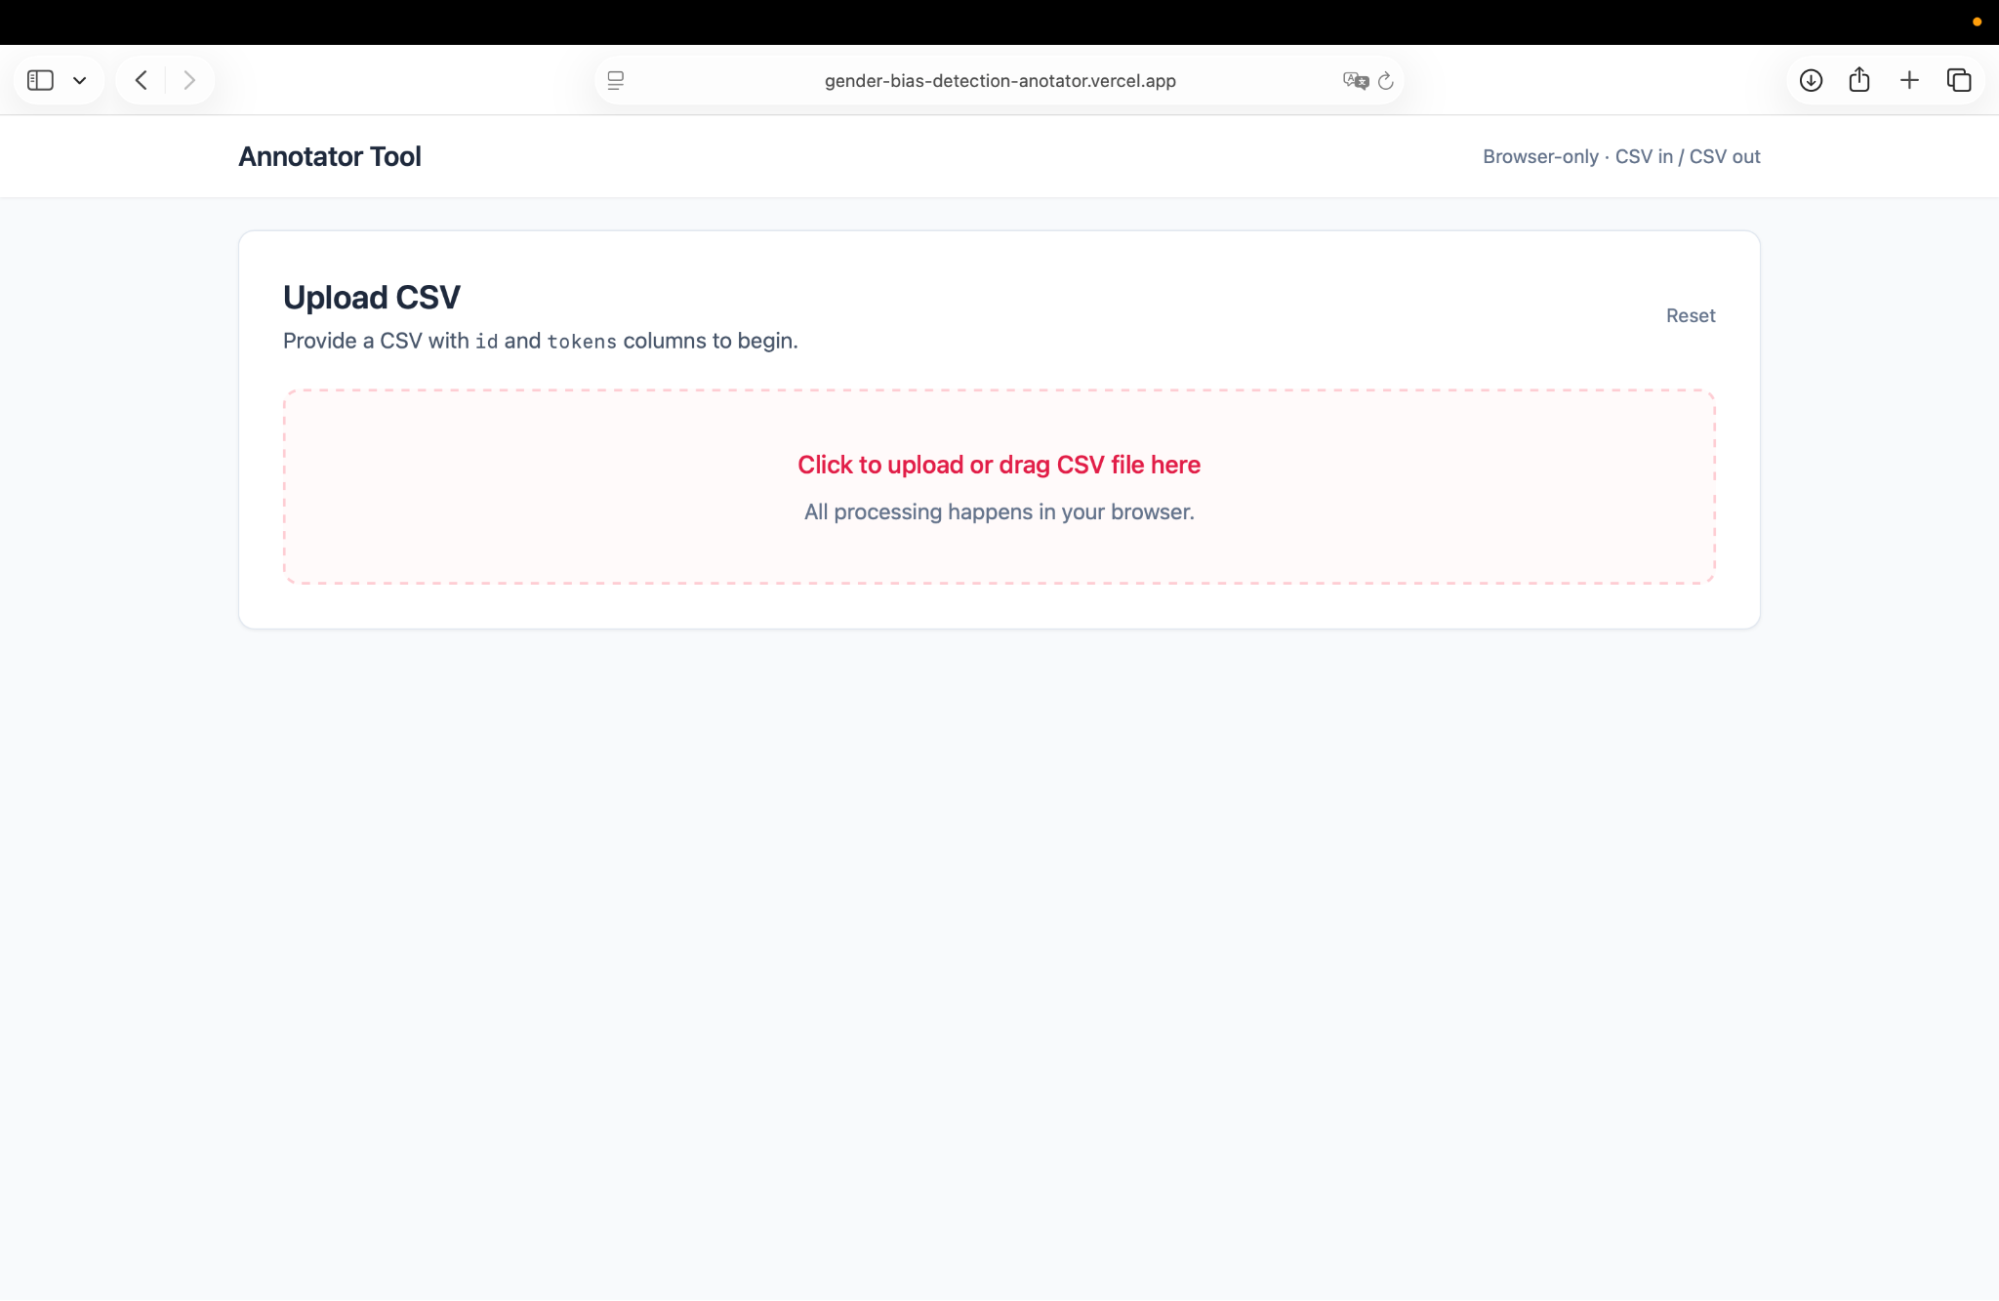
\includegraphics[width=0.8\linewidth]{assets/images/annotator_upload_csv.png}
\caption{Annotator Website - Upload CSV box}
\label{fig:annotator-upload-csv}
\end{figure}



\begin{figure}[H]
\centering
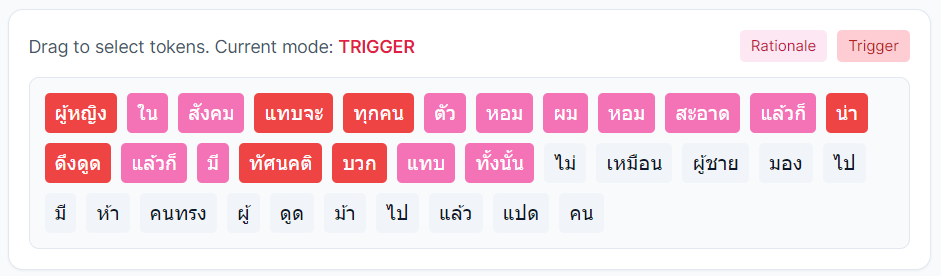
\includegraphics[width=0.8\linewidth]{assets/images/annotator_highlight_tokens.png}
\caption{Annotator Website - Highlight tokens box showing tokens in sequence}
\label{fig:annotator-highlight-tokens}
\end{figure}


\begin{figure}[H]
\centering
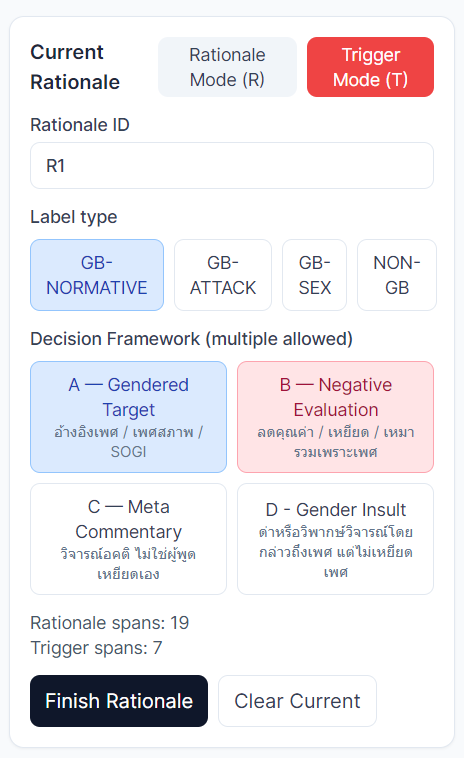
\includegraphics[width=0.8\linewidth]{assets/images/annotator_decision_box.png}
\caption{Annotator Website - Decision Annotate box}
\label{fig:annotator-decision-box}
\end{figure}



\begin{figure}[H]
\centering
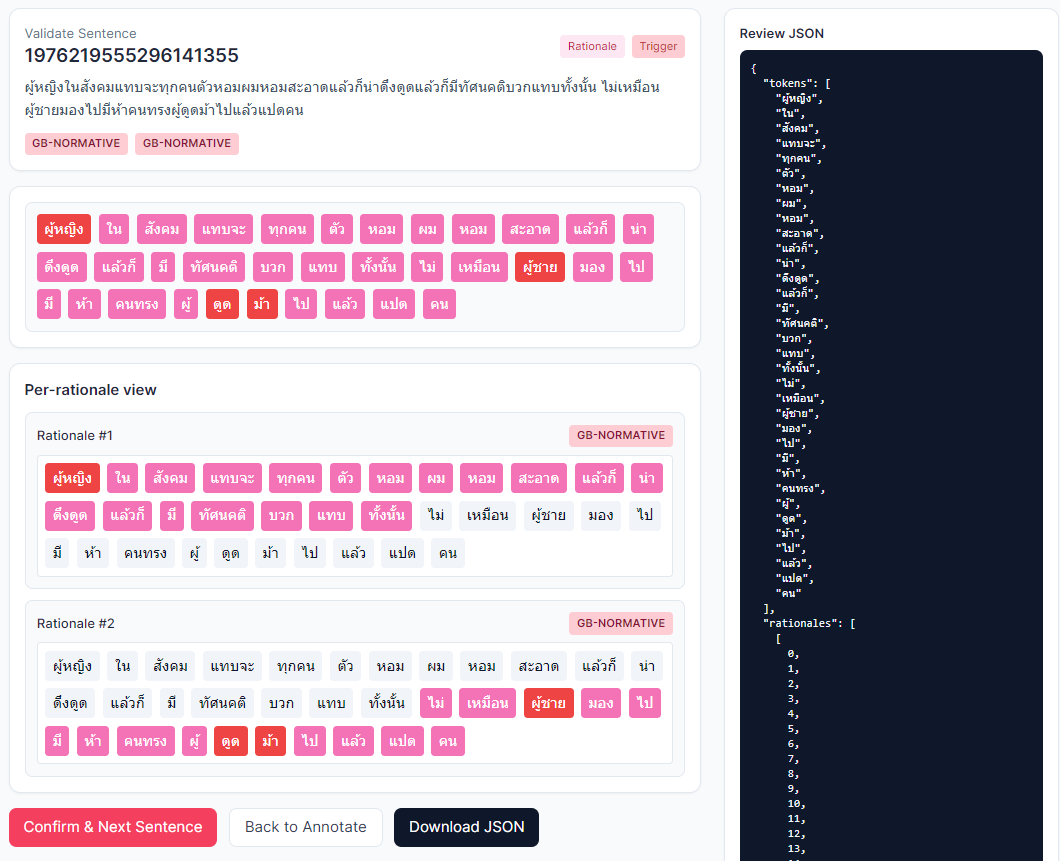
\includegraphics[width=0.8\linewidth]{assets/images/annotator_preview_page.png}
\caption{Annotator Website - Preview Page}
\label{fig:annotator-preview-page}
\end{figure}



\begin{figure}[H]
\centering
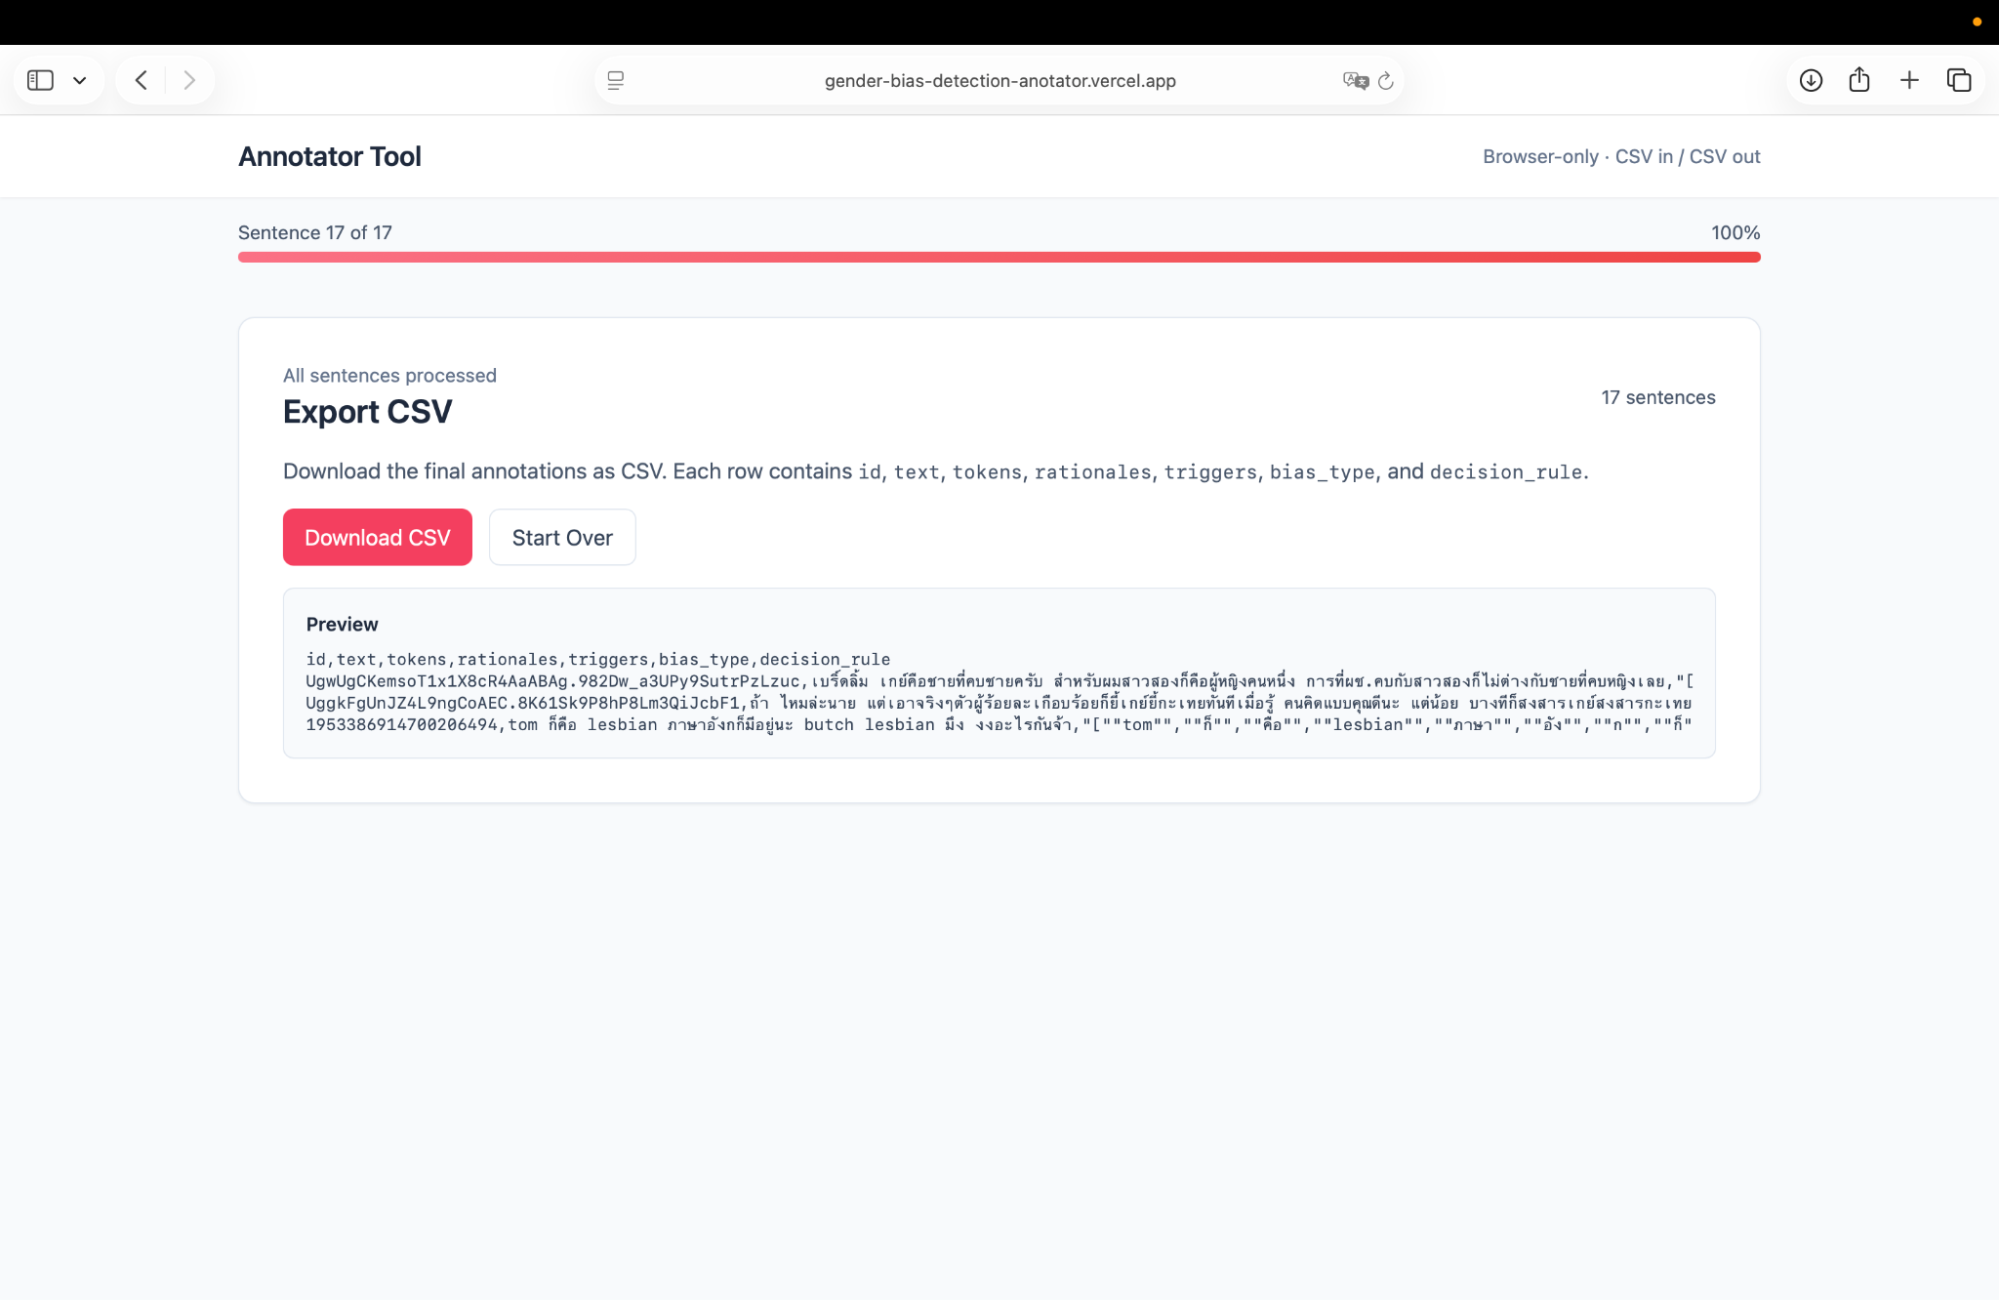
\includegraphics[width=0.8\linewidth]{assets/images/annotator_export_csv.png}
\caption{Annotator Website - Export CSV Page}
\label{fig:annotator-export-csv}
\end{figure}



\section{Synthetic Data Generation}

After annotation, the dataset showed class imbalance, with some gender-bias subtypes appearing much less frequently than others. This imbalance can affect model training because the model may become biased toward majority classes and perform poorly on minority categories, such as GB-SEX or less common SOGI-related bias.

To address this issue, synthetic data generation was added to the pipeline. Gemini 2.5 Flash was used through the synthesizer\_v2 pipeline to generate Thai social-media-style sentences based on the project's annotation guideline. The generated data covered the sentence-level label space used in this project, including GB-ATTACK, GB-NORMATIVE, GB-SEX, neutral, meta\_counter, and gendered\_insult. For the sentence-level model, the final synthetic training corpus contained 4,000 samples per class, resulting in 24,000 samples in total. This balanced structure was intended to reduce class imbalance during model training and provide more examples for underrepresented bias patterns.

The synthetic data were used as supporting training data rather than as the sole basis for evaluation. Human-annotated data remained essential for validation and final evaluation because it better reflects real Thai social-media language, including slang, ambiguity, and context-dependent expressions.

\section{Model Training}

\begin{figure}[H]
\centering
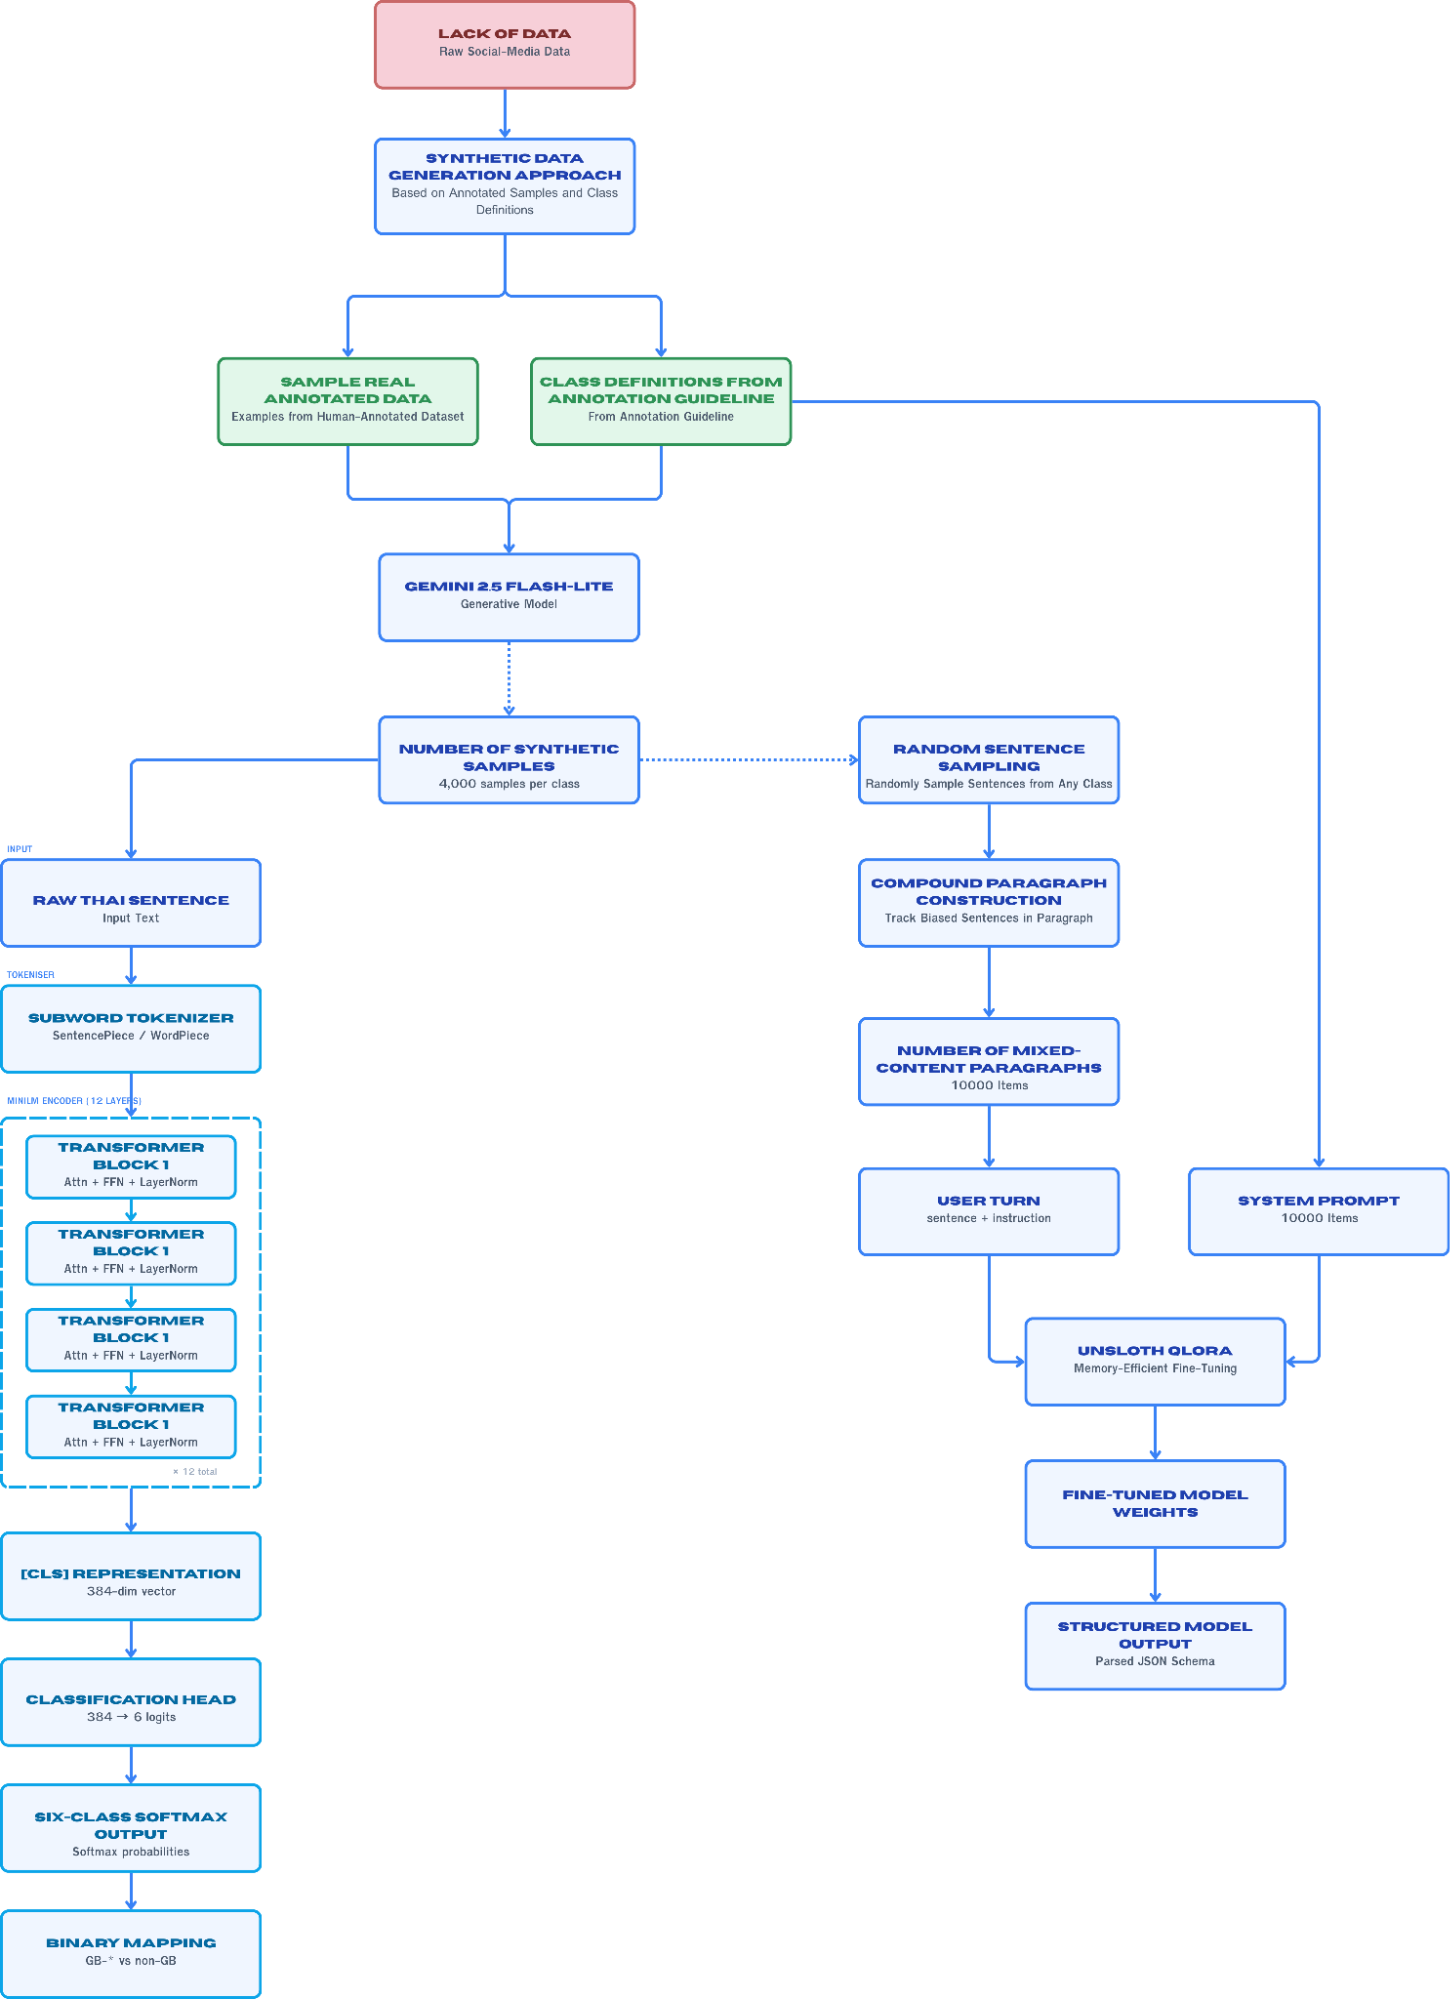
\includegraphics[width=0.8\linewidth]{assets/images/model_training_overview.png}
\caption{Model Traing Overview}
\label{fig:model-training-overview}
\end{figure}


\subsection{Sentence-Level Model}

Figure~\ref{fig:model-training-overview} shows the modelling framework, which consists of two levels: sentence-level classification and span-level detection. The sentence-level model is responsible for predicting a label for the entire input sentence, while the span-level model is intended to identify the specific words or phrases that support the prediction. This section focuses on the sentence-level classification component.

\subsubsection{Model Selection}

For the sentence-level classification task, this project uses microsoft/Multilingual-MiniLM-L12-H384~as the backbone encoder. Multilingual MiniLM is a compact BERT-style Transformer encoder that is distilled from larger Transformer models. It contains 12 layers with a hidden size of 384, providing a favourable balance between computational efficiency and representation quality. This makes it suitable for short and informal social-media text, where efficient inference is important.

Since the model was pre-trained on multilingual data, including Thai, it is able to capture subword-level patterns across languages without requiring a language-specific tokenizer. This is especially useful for Thai social-media text, which often contains informal spelling, slang, abbreviations, and mixed-language expressions.

The task is formulated as a six-class sequence classification problem. Each input sentence is assigned one of the following labels: GB-ATTACK,~GB-NORMATIVE, GB-SEX,~neutral,~meta\_counter, or gendered\_insult. The three GB-*~labels represent different forms of gender bias: direct attacks or dehumanisation, normative gender-role enforcement, and sexualised or body-based bias. The remaining three labels represent non-gender-biased cases, including neutral content, counter-speech or gender-awareness commentary, and insults that use gendered language without expressing gender bias.

In addition to the six-class setting, a binary Bias / Not-Bias view is derived from the same labels. The three GB-*~classes are grouped as Bias, while neutral, meta\_counter, and gendered\_insult are grouped as Not-Bias. Since this is a sentence-level model, the output is one predicted class for the entire sentence. The model does not identify rationale or trigger spans; these are handled separately in the span-level component.

\subsubsection{Training Data}

The sentence-level model was trained using the balanced synthetic corpus described in Section 3.6. This corpus contains 24,000 Thai social-media-style sentences, with 4,000 samples for each of the six sentence-level classes: GB-ATTACK, GB-NORMATIVE, GB-SEX, neutral, meta\_counter, and gendered\_insult.

Before training, the synthetic corpus was passed through a quality-filtering process. Texts shorter than 10 characters, texts longer than 512 characters, texts with a Thai character ratio below 20\%, and exact duplicate entries were removed. In this run, no samples were removed, indicating that the generated data satisfied the filtering criteria.

A key design decision was to use the human-annotated dataset as a hard validation set instead of holding out a random portion of the synthetic data. Validation on synthetic data from the same generator can produce inflated results because the model may learn recurring template patterns rather than robust semantic features of gender bias. Therefore, human-annotated data was used to provide a more realistic validation signal and to guide early stopping based on real examples.

The annotated dataset used for validation contains both GB and NON-GB examples. For six-class subtype validation, only rows with labels that map clearly to the six sentence-level classes are used. Rows labelled only as NON-GB~are retained for binary GB / NON-GB evaluation but excluded from six-class F1 computation because they may correspond to multiple non-bias categories, such as neutral content, counter-speech, or single-person gendered insults.

\subsubsection{Hyperparameters and Training Configuration}

\begin{table}[H]
\centering
\small
\caption{Hyperparameters and Training Configuration}
\begin{tabularx}{\textwidth}{@{}>{\raggedright\arraybackslash}p{0.38\textwidth}>{\raggedright\arraybackslash}X@{}}
\toprule
\textbf{Hyperparameter} & \textbf{Value} \\
\midrule
Base model & \url{microsoft/Multilingual-MiniLM-L12-H384} \\
Maximum sequence length & 128 tokens \\
Training batch size & 64 \\
Evaluation batch size & 128 \\
Learning rate & $2 \times 10^{-5}$ \\
Weight decay & 0.01 \\
Warmup ratio & 10\% of total training steps \\
Maximum epochs & 5 \\
Early-stopping patience & 2 epochs \\
Checkpoint selection metric & Hard-validation macro-F1 \\
Precision & FP16 mixed precision \\
Optimiser & AdamW, HuggingFace default \\
\bottomrule
\end{tabularx}
\end{table}

Training was implemented using the HuggingFace Trainer API. The \texttt{load\_best\_model\_at\_end} option was enabled, meaning that the checkpoint with the highest macro-F1 score on the hard validation set was selected as the final model. Early stopping was applied with a patience of two epochs. If the hard-validation macro-F1 score did not improve for two consecutive epochs, training was terminated to reduce overfitting to the synthetic training distribution.

Each input sentence was tokenized using the pretrained MiniLM tokenizer and padded or truncated to a maximum length of 128 tokens. The model receives input\_ids and attention\_mask as input features, while the target label is converted into a numeric class ID using a fixed label-to-ID mapping. A sequence-classification head is added on top of the MiniLM encoder, and the model is trained using cross-entropy loss, where each sentence has one ground-truth class label.

During validation, accuracy, macro-precision, macro-recall, and macro-F1 are computed. Macro-F1 is used as the main checkpoint-selection metric because it gives equal weight to all classes and is more suitable for imbalanced class distributions.

\subsection{Span-Level Model}

The span-level model is designed to identify the specific words or phrases that express gender bias within an input text. Unlike the sentence-level model, which predicts one label for the whole sentence, the span-level model extracts biased spans and assigns them to one of the GB subtypes: GB-ATTACK, GB-NORMATIVE, or GB-SEX. This component improves model interpretability by identifying the text spans that support the bias prediction, rather than only producing a sentence-level label.

\subsubsection{Initial BIO Tagging Design}

The initial span-level detection approach treated the task as a token-level sequence labeling problem, similar to Named Entity Recognition. Under this design, each token would be assigned a BIO tag indicating whether it begins a biased span, continues a biased span, or is outside any biased span. The planned tag set included B-GB-ATTACK, I-GB-ATTACK, B-GB-NORMATIVE, I-GB-NORMATIVE, B-GB-SEX, I-GB-SEX, and O.

A transformer encoder such as WangchanBERTa would then be fine-tuned to predict a tag for each token. After prediction, consecutive B and I tags could be reconstructed into biased text spans. This approach is conceptually suitable for span detection because it directly aligns model predictions with token-level annotations.

However, this approach was not used in the final span-level implementation due to data limitations. Token-level sequence labeling requires a large amount of reliable span-annotated data, since every token in every sentence must have a gold label. At the current stage, the available human-annotated span-level dataset is still limited. In addition, the sentence-level model already showed difficulty with stance-sensitive and implicit bias cases, suggesting that a token-level encoder model trained on limited real-world data would likely face even greater challenges. Therefore, BIO tagging was kept as an initial design but not selected as the final span-level approach.

\subsubsection{LoRA-Based Generative Span Extraction Design}

To address the limitations of BIO tagging, the span-level approach was revised to use a small generative language model fine-tuned with LoRA. A generative model was selected because it can use its pretrained language knowledge to extract spans from text even when supervised span-level data is limited. LoRA was used to make fine-tuning more efficient by updating only a small number of adapter parameters instead of the full model.

The model size was limited to approximately 2–4 billion parameters to support the project’s long-term goal of lightweight deployment, such as a browser extension or low-resource inference environment. Candidate backbone models were selected from the Qwen 3.5 family, specifically the 2B and 4B parameter variants. These models were chosen because they provide a balance between multilingual capability, instruction-following performance, and computational efficiency while remaining feasible for deployment on resource-constrained hardware.

Two backbone models, Qwen3.5-2B and Qwen3.5-4B, were evaluated for the span-level extraction task. The 2B model represents a lightweight configuration with lower memory and computational requirements, while the 4B model provides increased model capacity that may improve extraction performance at the cost of additional resources. Comparing both configurations allows the trade-off between model efficiency and extraction quality to be assessed.

Fine-tuning was conducted using the Unsloth framework \hyperlink{bib:ref49}{[49]}. Unsloth was used because it provides optimized model loading, 4-bit quantized checkpoints, LoRA adapter support, and memory-efficient training. This allowed the model to be fine-tuned under limited GPU resources while still applying the same LoRA-based training procedure to the selected Qwen model.

\subsubsection{LoRA Hyperparameters and Training Configuration}

Table~\ref{tab:span-lora-training-config} summarizes the LoRA fine-tuning configuration used for the span-level generative model. Unlike QLoRA-style low-bit training, this configuration used 16-bit LoRA because the RTX 6000 Blackwell GPU provided sufficient VRAM for higher precision. The goal was to preserve span extraction accuracy while still updating only the LoRA adapter parameters rather than the full model.

\begin{table}[H]
\centering
\small
\caption{LoRA Hyperparameters and Training Configuration for the Span-Level Model}
\label{tab:span-lora-training-config}
\begin{tabularx}{\textwidth}{@{}>{\raggedright\arraybackslash}p{0.38\textwidth}>{\raggedright\arraybackslash}X@{}}
\toprule
\textbf{Hyperparameter} & \textbf{Value} \\
\midrule
Candidate backbone models & Qwen 3.5 2B and Qwen 3.5 4B range \\
Maximum sequence length & 4096 tokens \\
Fine-tuning method & LoRA with Unsloth \\
Quantization & Disabled; 16-bit LoRA instead of QLoRA \\
Precision & BF16 mixed precision \\
LoRA rank & 128 \\
LoRA alpha & 256 \\
LoRA dropout & 0.05 \\
Target modules & \texttt{q\_proj}, \texttt{k\_proj}, \texttt{v\_proj}, \texttt{o\_proj}, \texttt{gate\_proj}, \texttt{up\_proj}, \texttt{down\_proj} \\
Special span tokens & \texttt{<GB-ATTACK>}, \texttt{</GB-ATTACK>}, \texttt{<GB-NORMATIVE>}, \texttt{</GB-NORMATIVE>}, \texttt{<GB-SEX>}, \texttt{</GB-SEX>} \\
Training batch size & 64 \\
Evaluation batch size & 64 \\
Gradient accumulation steps & 1 \\
Learning rate & $2 \times 10^{-4}$ \\
Weight decay & 0.01 \\
Warmup steps & 100 \\
Maximum epochs & 3 \\
Evaluation strategy & Every 100 steps \\
Checkpoint strategy & Save every 100 steps; keep latest 2 checkpoints \\
Optimizer & \texttt{adamw\_8bit} \\
Packing & Disabled to preserve span-level alignment \\
Random seed & 42 \\
Training hardware & RTX 6000 Blackwell, 96 GB VRAM \\
\bottomrule
\end{tabularx}
\end{table}

\subsubsection{Training Data Construction}

The span-level training data was constructed as mixed-content documents rather than isolated single-sentence examples. This design was chosen because real social media posts often contain a mixture of biased and non-biased sentences within the same comment, thread, or post. Training only on isolated biased sentences may not reflect this realistic structure.

Instead of generating a new synthetic sentence pool specifically for span-level training, the span-level dataset was built from available sentence-level data. Existing sentences from GB and NON-GB categories were reused and combined into paragraph-like inputs. These mixed-content documents were created by randomly sampling and concatenating 1--20 sentences per example. Approximately 20--40\% of the sentences were drawn from bias categories, while 60--80\% were drawn from non-bias categories. The sentences were then shuffled into a natural order to simulate social media text where biased and neutral content may appear together. Bias labels were preserved during this process so that the model could learn which parts of the mixed input contained gender-biased content.

The resulting corpus contained 10,000 mixed-content examples. These were divided into 9,500 training examples and 500 validation examples using stratified sampling based on the primary bias type present in each document. This helped preserve the distribution of GB-ATTACK, GB-NORMATIVE, GB-SEX, and NON-GB examples across the training and validation sets.

\subsubsection{Output Format Design}

A major challenge in span-level extraction was designing an output format that the generative model could follow consistently. The first approach used XML-style inline tagging, where the model reproduced the input text and wrapped biased spans with tags such as \texttt{<GB-NORMATIVE>}\ldots\texttt{</GB-NORMATIVE>}, \texttt{<GB-ATTACK>}\ldots\texttt{</GB-ATTACK>}, or \texttt{<GB-SEX>}\ldots\texttt{</GB-SEX>}. This format was intuitive because it marked biased spans directly inside the original text.

However, XML-style tagging was inconsistent in practice. The model sometimes produced malformed tags, added explanations, or inserted extra commentary instead of only extracting the biased spans. Since generative models are trained to produce fluent text, open-ended tag-based outputs created ambiguity between extraction and explanation.

To improve consistency, the output format was revised to structured JSON. Instead of generating annotated text, the model is instructed to return a fixed JSON object with exactly three keys: GB-NORMATIVE, GB-SEX, and GB-ATTACK. Each key maps to a list of extracted span strings copied directly from the input text. The prompt explicitly prohibits explanations, markdown, and additional keys, and requires the output to be parseable as JSON.

This structured output format reduces formatting errors and makes the model output easier to use in downstream evaluation. It also supports automatic comparison with human-annotated spans because the extracted strings are grouped by GB subtype.

\subsubsection{Prompt and Fine-Tuning Setup}

The model was trained using the ChatML instruction format. The system prompt includes the full annotation guideline, including the decision criteria A--D, span selection rules, and examples of both bias-present and bias-absent inputs. The prompt was written in Thai to match the language of the input data and reduce the burden of switching between Thai social media text and English instructions.

During training, the user input consists of the original untagged text, while the assistant target output is the structured JSON object containing extracted spans. For quality control, the generated training examples were checked to ensure that the input text contained no tags, the output followed the expected structure, and extracted spans were copied from the input rather than hallucinated.

This span-level model remains under development and is evaluated separately from the sentence-level classifier. Its purpose is to support interpretable gender-bias detection by extracting the text spans that correspond to each GB subtype.

\subsection{Model Training Environment}

Separate training environments were used for the sentence-level and span-level models because the two tasks have different computational requirements. Sentence-level classification uses a smaller encoder-based model and requires less GPU memory, while span-level extraction uses a larger generative model with LoRA fine-tuning and therefore requires stronger hardware support.

\subsubsection{Sentence-Level Training Environment}

The sentence-level classification model was trained in Google Colab using a free-tier T4-class GPU. This environment was sufficient because the model uses a lightweight MiniLM-class encoder, a short maximum sequence length, and a standard sequence classification objective. Since each input receives only one sentence-level label, the training process is less memory-intensive than span-level generative fine-tuning.

The sentence-level training setup has the following characteristics:

\begin{table}[H]
\centering
\small
\caption{Sentence-Level Training Configuration Characteristics}
\begin{tabularx}{\textwidth}{@{}>{\raggedright\arraybackslash}p{0.34\textwidth}>{\raggedright\arraybackslash}X@{}}
\toprule
\textbf{Component} & \textbf{Description} \\
\midrule
Training platform & Google Colab Free Tier \\
GPU class & T4-class GPU \\
Model type & Small-to-medium encoder backbone \\
Training objective & Sequence classification \\
Output type & Single label per input sentence \\
Maximum sequence length & 128 tokens \\
Main purpose & Low-cost baseline training, debugging, and hyperparameter tuning \\
\bottomrule
\end{tabularx}
\end{table}

\subsubsection{Span-Level Training Environment}

The span-level model requires a stronger training environment because it uses a generative model for span extraction. Unlike sentence-level classification, span-level detection requires the model to generate structured outputs and learn span-aware behavior. This increases memory usage, especially when working with billion-parameter models and chat-style supervision.

For this task, a dedicated GPU virtual machine on Vast.ai was selected. Although memory optimization techniques such as quantization and Unsloth-based LoRA fine-tuning reduce GPU usage, stable training still requires more VRAM than what is typically available in free-tier notebook environments.

The main reasons for using a dedicated GPU VM are:

\begin{table}[H]
\centering
\small
\caption{Span-Level Training Environment Requirements and Justifications}
\begin{tabularx}{\textwidth}{@{}>{\raggedright\arraybackslash}p{0.34\textwidth}>{\raggedright\arraybackslash}X@{}}
\toprule
\textbf{Requirement} & \textbf{Reason} \\
\midrule
Higher VRAM & Reduces out-of-memory risk during LoRA fine-tuning and provides runtime memory headroom \\
Larger model support & Allows training of billion-parameter generative models \\
Longer sequence handling & Supports longer inputs, chat-style supervision, and structured output generation \\
Training stability & Provides more reliable resources for sustained fine-tuning jobs \\
\bottomrule
\end{tabularx}
\end{table}

\subsubsection{VM Platform Selection and Cost Consideration}

Vast.ai was selected for span-level training because it provides access to high-VRAM GPU instances at a lower rental cost compared with many standard cloud platforms. This made it more suitable for an academic project with limited budget and experimental training needs.

The platform was selected based on the following criteria:

\begin{table}[H]
\centering
\small
\caption{VM Platform Selection Criteria for Span-Level Training}
\begin{tabularx}{\textwidth}{@{}>{\raggedright\arraybackslash}p{0.34\textwidth}>{\raggedright\arraybackslash}X@{}}
\toprule
\textbf{Criterion} & \textbf{Explanation} \\
\midrule
Cost efficiency & Supports long-running fine-tuning jobs at lower cost \\
High-VRAM availability & Provides GPUs suitable for LLM adaptation \\
Flexible instance selection & Allows different GPU configurations to be tested \\
Budget-performance balance & Fits the hardware needs of the project while controlling cost \\
\bottomrule
\end{tabularx}
\end{table}

\subsubsection{Target GPU Specification for Span-Level Fine-Tuning}

To support stable span-level fine-tuning, the project sets a minimum GPU memory requirement of 32 GB VRAM. Datacenter-grade GPUs are preferred over consumer RTX or GTX GPUs because they are more stable for sustained training workloads and usually provide better memory capacity.


\begin{table}[H]
\centering
\small
\caption{Target GPU Specifications for Span-Level Fine-Tuning}
\begin{tabularx}{\textwidth}{@{}>{\raggedright\arraybackslash}p{0.34\textwidth}>{\raggedright\arraybackslash}X@{}}
\toprule
\textbf{Specification} & \textbf{Requirement} \\
\midrule
Minimum GPU VRAM & At least 32 GB \\
Preferred GPU type & Datacenter-grade GPU \\
Recommended GPU class & NVIDIA A100, 40 GB or higher preferred \\
Additional system support & Sufficient CPU RAM and storage for preprocessing, checkpoints, and logs \\
\bottomrule
\end{tabularx}
\end{table}

\section{Evaluation}

The evaluation stage assesses the performance and interpretability of the gender-bias detection system on human-annotated data. In the current experiment, the sentence-level model is trained using synthetic data, while real human-annotated samples are used as a hard validation set. This setup measures how well the model generalizes from generated examples to actual Thai social-media language, including informal wording, slang, implicit bias, neutral gender mentions, counter-speech, and context-dependent expressions.

For sentence-level evaluation, the model is assessed in two settings. The first is binary classification, where the three bias labels, GB-ATTACK, GB-NORMATIVE, and GB-SEX, are grouped as GB, while non-bias labels are grouped as NON-GB. This evaluation measures the model's ability to detect whether gender bias is present in a sentence.

The second setting is subtype classification, which evaluates whether the model can correctly distinguish between GB-ATTACK, GB-NORMATIVE, and GB-SEX. This is important because the system should not only detect the presence of gender bias, but also identify the form of harm being expressed, such as direct attacks, gender-role enforcement, or sexualized and body-based bias.

For span-level evaluation, model-predicted extracted spans are compared with human-annotated GB spans. Since the current span-level model produces structured JSON outputs grouped by GB subtype, the evaluation focuses on whether the extracted span strings match the annotated biased spans for GB-ATTACK, GB-NORMATIVE, and GB-SEX. The evaluation is conducted mainly on GB rows because NON-GB rows do not contain ground-truth biased spans for extraction comparison.

Two complementary metrics are used: exact-match span F1 and character-level F1. Exact-match span F1 requires the predicted span to match the annotated span exactly, while character-level F1 gives partial credit when the model identifies the correct region but selects imperfect span boundaries. The gap between these two metrics helps diagnose whether errors are caused by incorrect bias localization or boundary mismatch. In addition, faithfulness rate is used to check whether the predicted spans are copied directly from the input text rather than hallucinated.

In addition to quantitative evaluation, error analysis is conducted by examining false positives, false negatives, label confusion, false alarms on NON-GB rows, and boundary-related errors. This helps identify common weaknesses such as over-extraction from neutral gender mentions, misclassification between GB subtypes, imprecise span boundaries, counter-speech misclassified as bias, implicit stereotypes, slang-based bias, and comments that require wider conversational context. These findings are used to guide future improvement of both the sentence-level and span-level components, especially by adding more human-annotated span examples and improving stance-sensitive detection.
\chapter{Results and Discussion}

\section{Data Collection}

\begin{figure}[H]
\centering
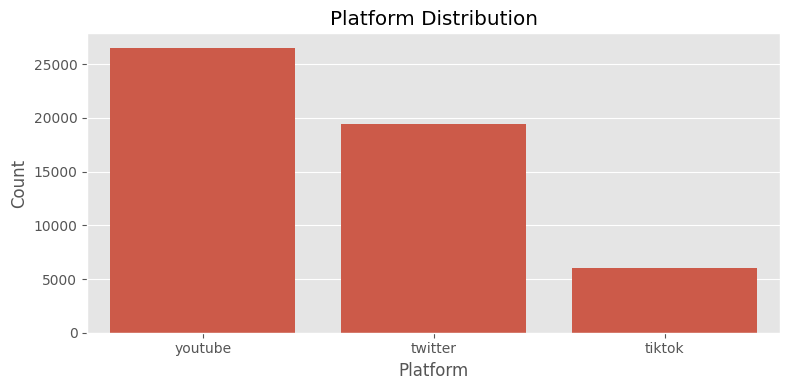
\includegraphics[width=0.8\linewidth]{assets/images/chapter4/image20.png}
\caption{Distribution of Data in YouTube, Twitter/X, and TikTok}
\label{fig:platform-data-distribution}
\end{figure}



Figure~\ref{fig:platform-data-distribution} shows the overall distribution of collected data across the three target platforms: YouTube, Twitter/X, and TikTok. In total, the data collection process produced 52,055 unique text records after deduplication. YouTube contributes the largest portion of the dataset with 26,546 comments, followed by Twitter/X with 19,454 text records, and TikTok with 6,055 comments. This distribution reflects the different characteristics of each platform. YouTube provides the largest amount of data because each video can contain many public comments, while Twitter/X contributes a large number of posts, replies, and quoted tweets from fast-moving discussions. TikTok has the smallest share because comments are generally shorter and fewer records were collected from the selected video IDs. Overall, the combined dataset provides diverse Thai social media text from both short reactive comments and longer discussion-based content, making it suitable for gender-bias analysis.

\subsection{Twitter/X (Selenium-based)}

From Twitter/X, the Selenium-based crawling pipeline collected Thai social media text from multiple content types, including original tweets, replies, and quoted or embedded tweets. This allowed the dataset to capture not only standalone posts but also conversational and reaction-based content, where gender-related expressions often appear. After deduplication, the Twitter/X dataset contained 19,454 unique text records.

Twitter/X is especially useful for gender-bias research because its content is highly informal and fast-moving. Posts and replies often contain strong opinions, slang, sarcasm, and direct interpersonal judgments, which can include both explicit and subtle gendered expressions.

\subsection{TikTok (TikTokApi):}

TikTok comments were collected using a TikTokApi-based scraping pipeline. The scraper retrieved user-generated comments from selected TikTok video IDs, including top-level comments and threaded replies when available. For each record, the pipeline stored the comment text, timestamp, and comment ID. After consolidation and deduplication, the TikTok dataset contained 6,055 unique comments, with the collected platform-type distribution shown in Figure~\ref{fig:tiktok-platform-type-distribution}.

TikTok comments are valuable for this project because they are usually short, reactive, and conversational. Compared with longer-form platforms, TikTok often contains immediate emotional responses, teasing, humor, and slang. These characteristics make the platform useful for observing informal gendered expressions and interpersonal judgments.

\begin{figure}[H]
\centering
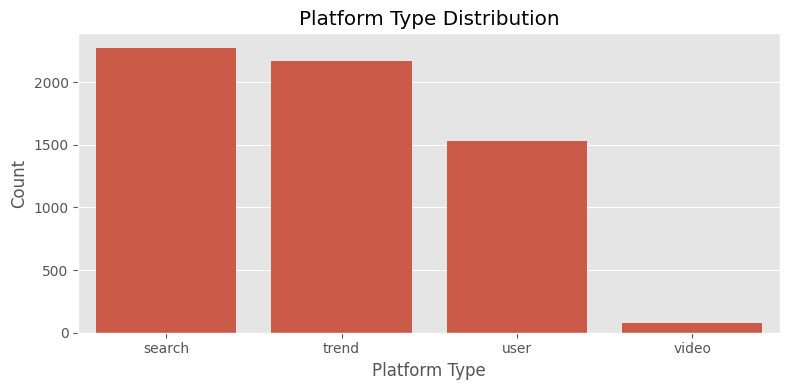
\includegraphics[width=0.8\linewidth]{assets/images/chapter4/image2.png}
\caption{Distribution of platform type from TikTok}
\label{fig:tiktok-platform-type-distribution}
\end{figure}

\subsection{YouTube (yt-dlp):}

YouTube comments were extracted using the \texttt{yt-dlp} framework, which allows access to public video metadata and retrievable top-level comments. The scraper collected comment text, timestamps, comment IDs, and video-related metadata from selected public videos. After preprocessing and deduplication, the YouTube dataset contained 26,546 unique comments.

YouTube contributes the largest portion of the dataset and provides a different style of social media discourse compared with Twitter/X and TikTok. Its comments are often longer, more narrative, and more discussion-based. This makes YouTube useful for collecting opinions, debates, social critique, and context-rich expressions that may not appear as frequently in shorter comment formats. Overall, YouTube adds diversity to the dataset by complementing the shorter and more reactive language found on Twitter/X and TikTok.



\section{Exploratory data analysis (EDA)}

\subsection{Social Media Dataset Wordcloud}

\begin{figure}[H]
\centering
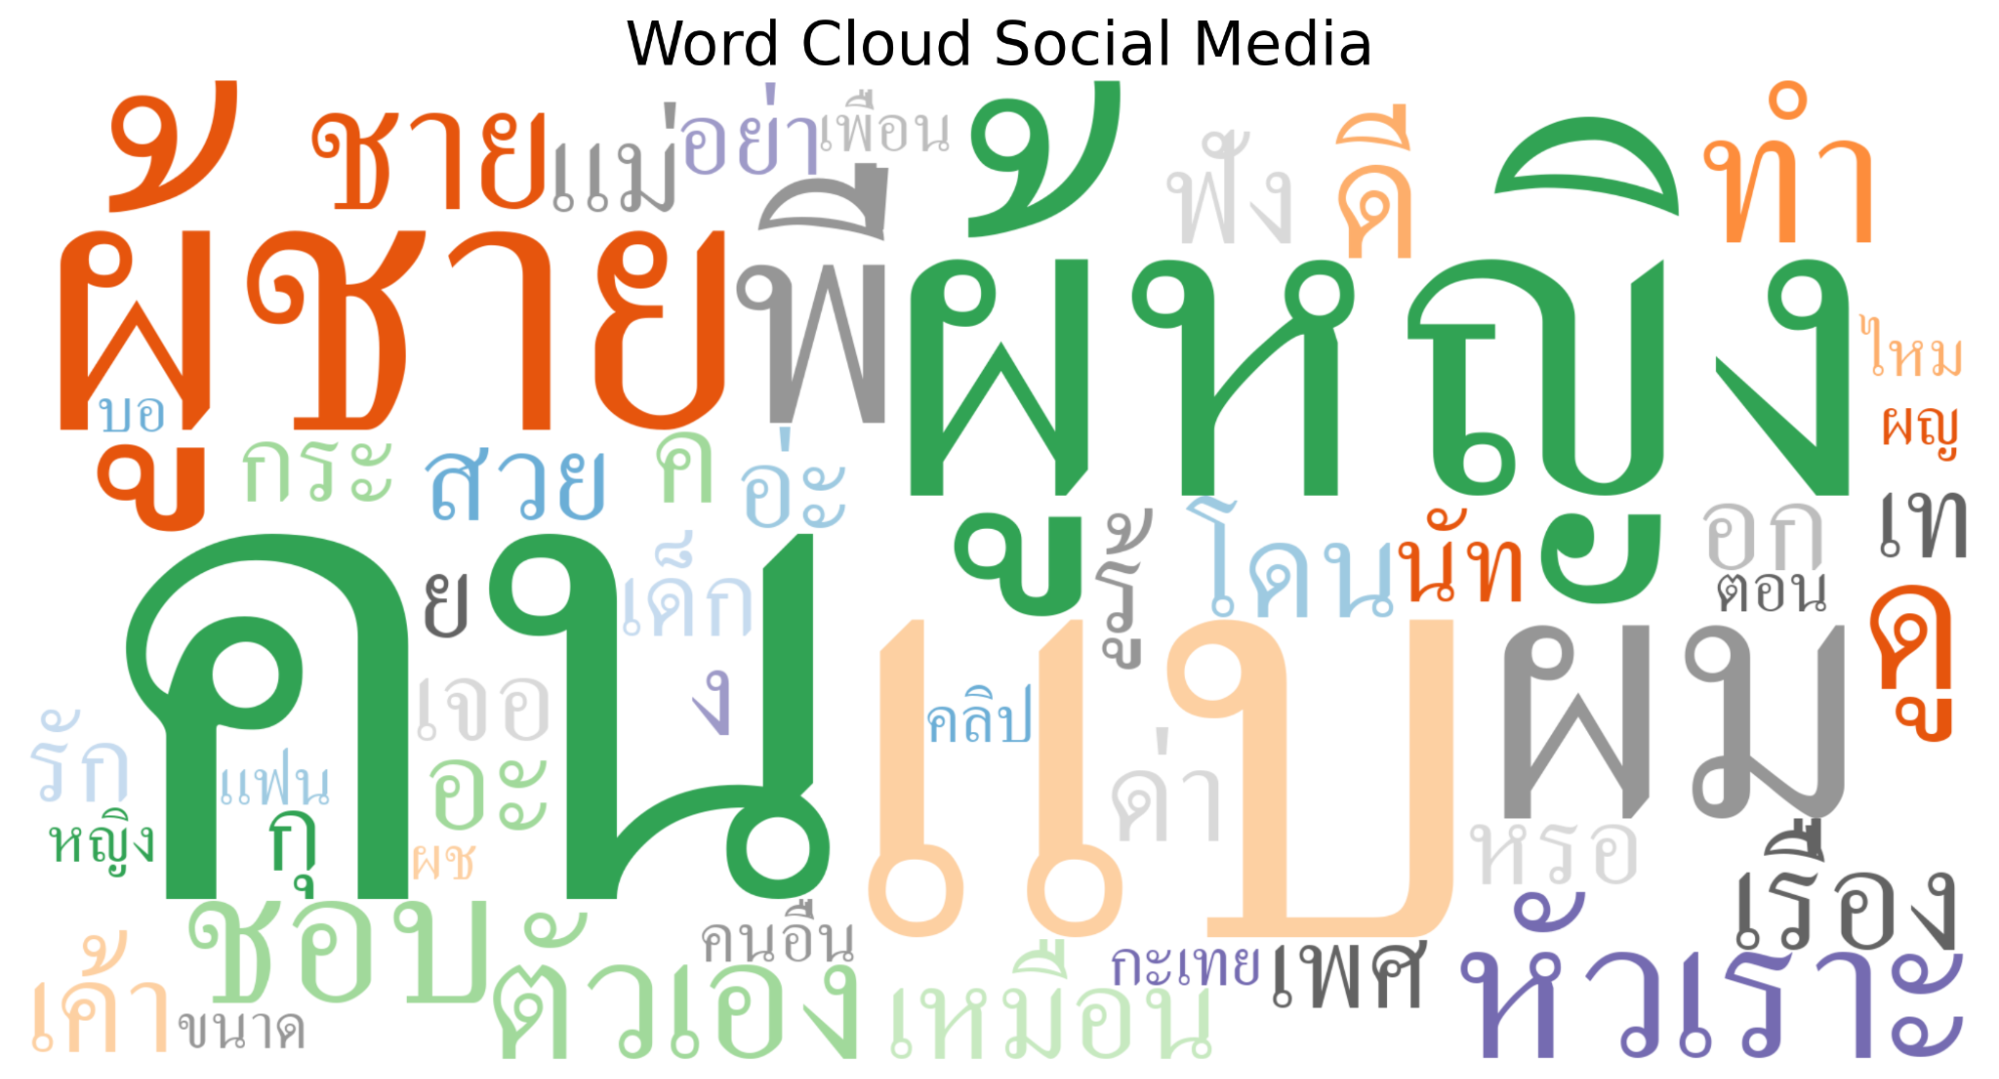
\includegraphics[width=0.8\linewidth]{assets/images/chapter4/image11.png}
\caption{Social Media Dataset Wordcloud}
\label{fig:social-media-dataset-wordcloud}
\end{figure}

The word cloud in Figure~\ref{fig:social-media-dataset-wordcloud} represents the overall dataset across all platforms, providing a high-level view of the most frequent lexical items. The most dominant terms are ``ผู้หญิง'' (woman), ``ผู้ชาย'' (man), ``คน'' (person), ``แฟน'' (partner), and ``ผม'' (I/male), indicating a strong focus on gender, identity, and interpersonal relationships across platforms. Other frequent terms such as ``สวย'' (beautiful), ``เพศ'' (gender), ``ด่า'' (insult), and ``หัวเราะ'' (laugh/lol) suggest the presence of evaluative, emotional, and potentially judgmental language.

The appearance of gendered terms across all parts of speech (nouns, pronouns, verbs) supports the dataset's relevance for gender-bias detection, particularly in informal and conversational contexts. Additionally, frequent emotional verbs (e.g., ``ชอบ'' -- like, ``ดู'' -- watch, ``ทำ'' -- do/make) point to the dataset's expressive nature and high engagement with personal or social commentary.

This confirms that the dataset contains rich, high-signal content for modeling bias, identity framing, and social attitudes in Thai social media discourse.

To illustrate platform-specific linguistic patterns and distinctions, separate word-frequency analyses for YouTube, Twitter/X, and TikTok are shown in Figure~\ref{fig:youtube-wordcloud}, Figure~\ref{fig:twitter-wordcloud}, and Figure~\ref{fig:tiktok-wordcloud}.





\begin{figure}[H]
\centering
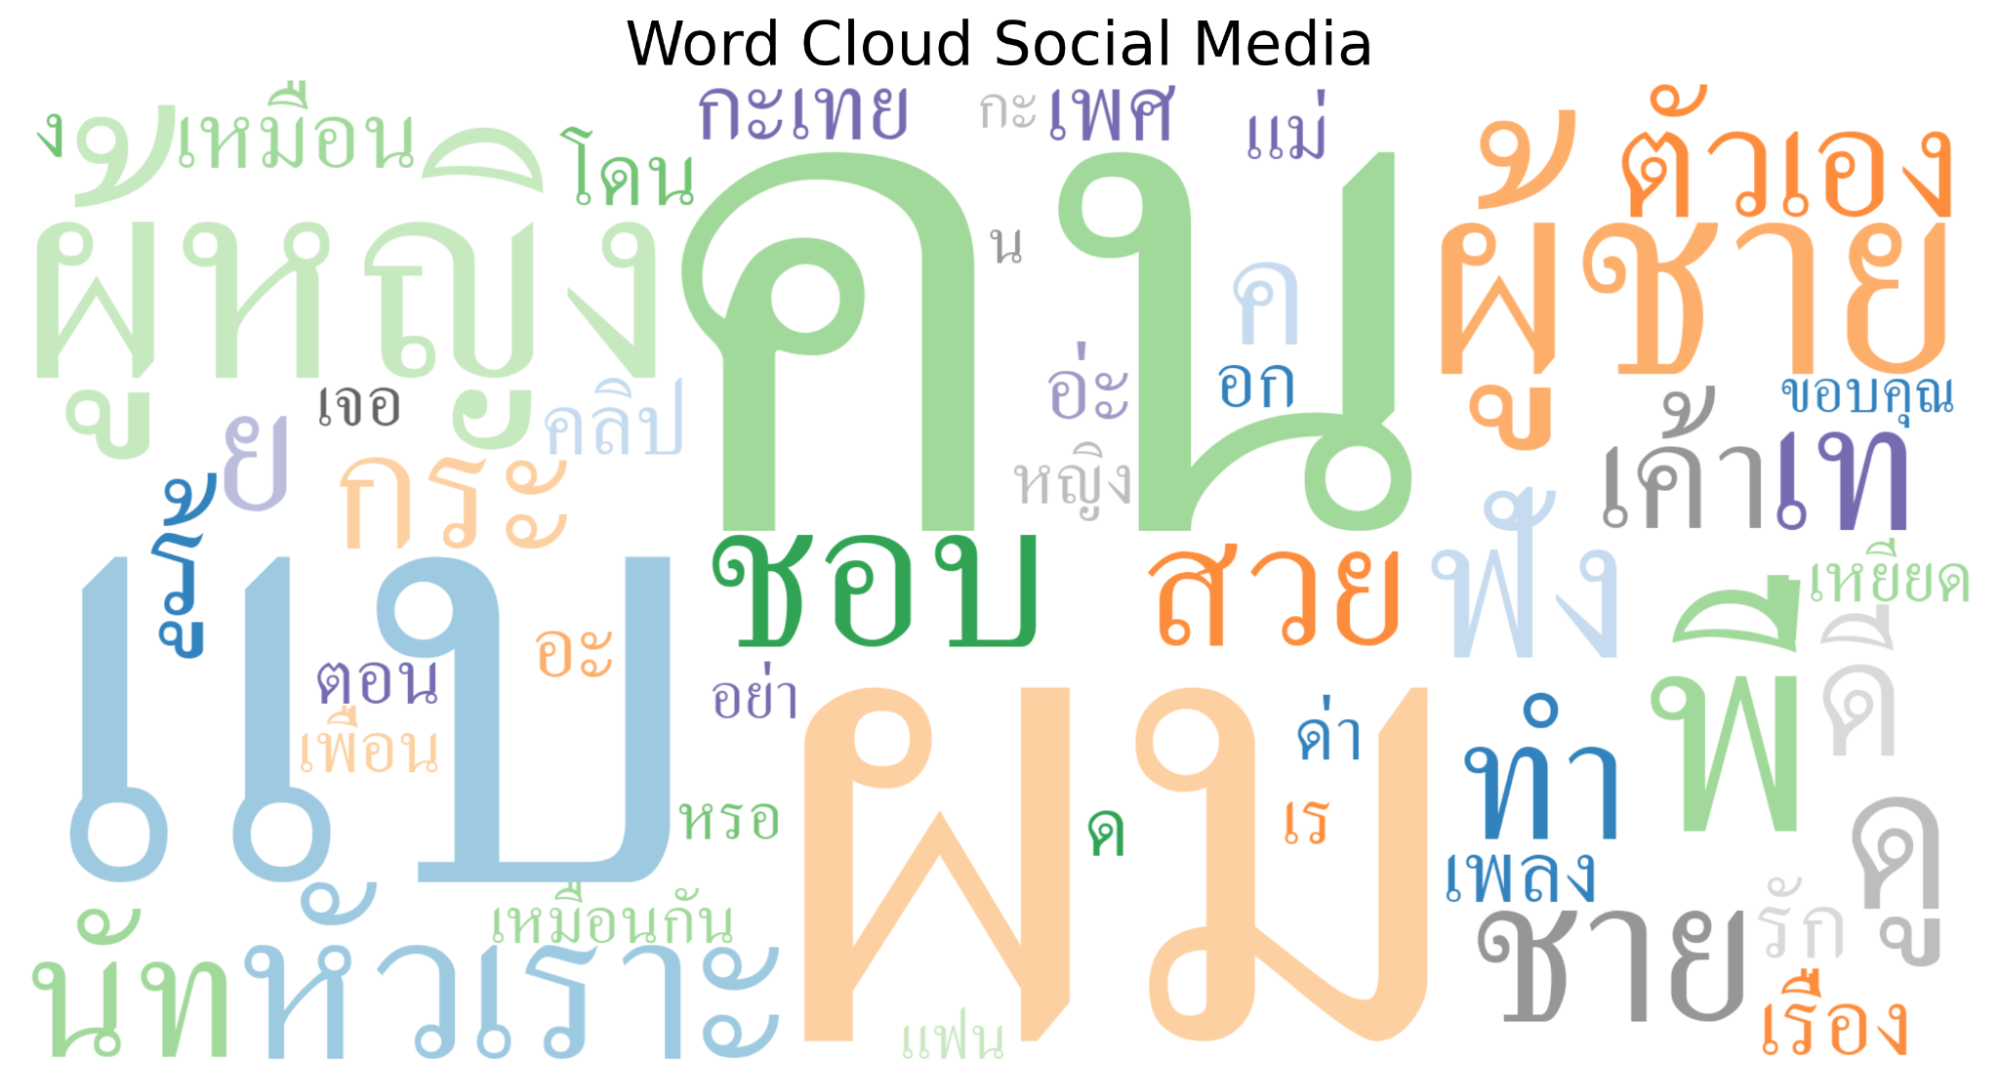
\includegraphics[width=0.8\linewidth]{assets/images/chapter4/image4.png}
\caption{Social Media Dataset Wordcloud (YouTube)}
\label{fig:youtube-wordcloud}
\end{figure}

\begin{figure}[H]
\centering
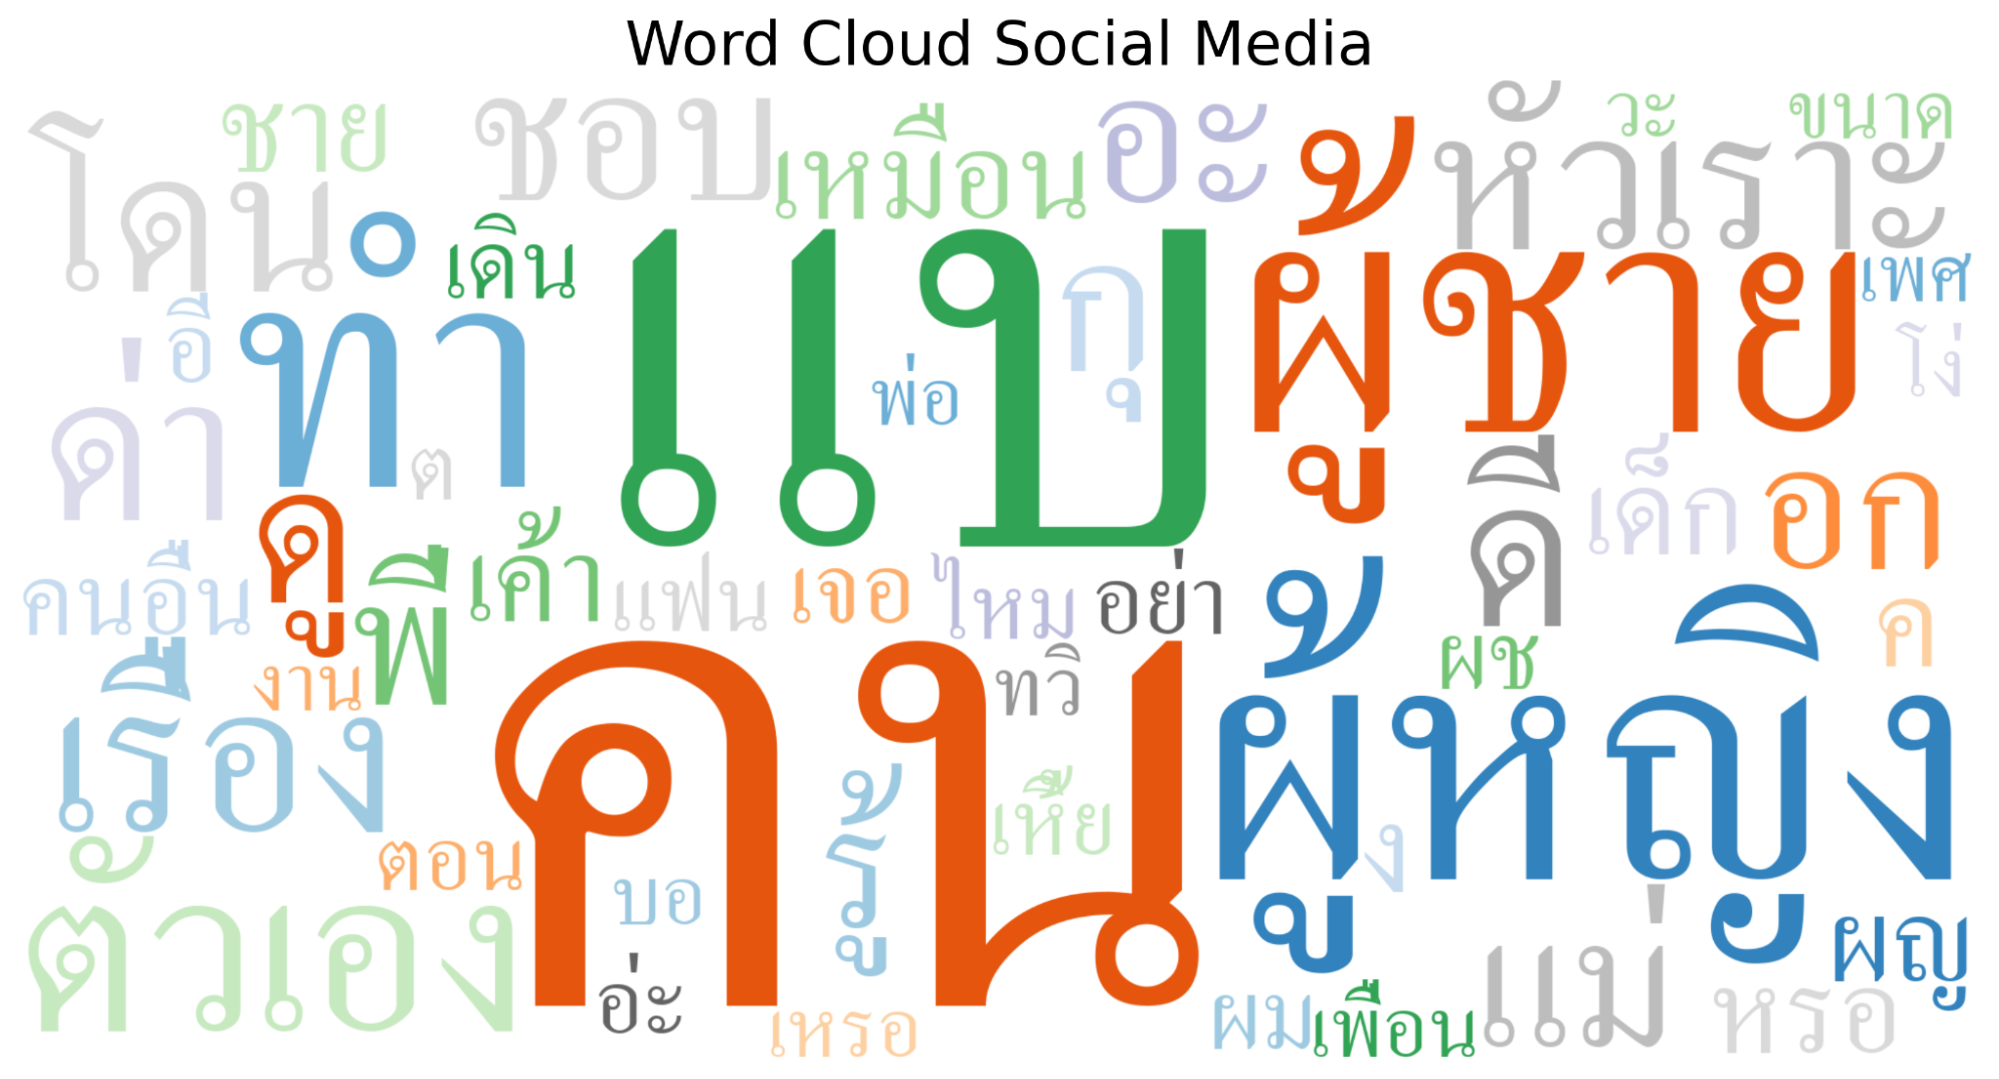
\includegraphics[width=0.8\linewidth]{assets/images/chapter4/image21.png}
\caption{Social Media Dataset Wordcloud (Twitter/X)}
\label{fig:twitter-wordcloud}
\end{figure}

\begin{figure}[H]
\centering
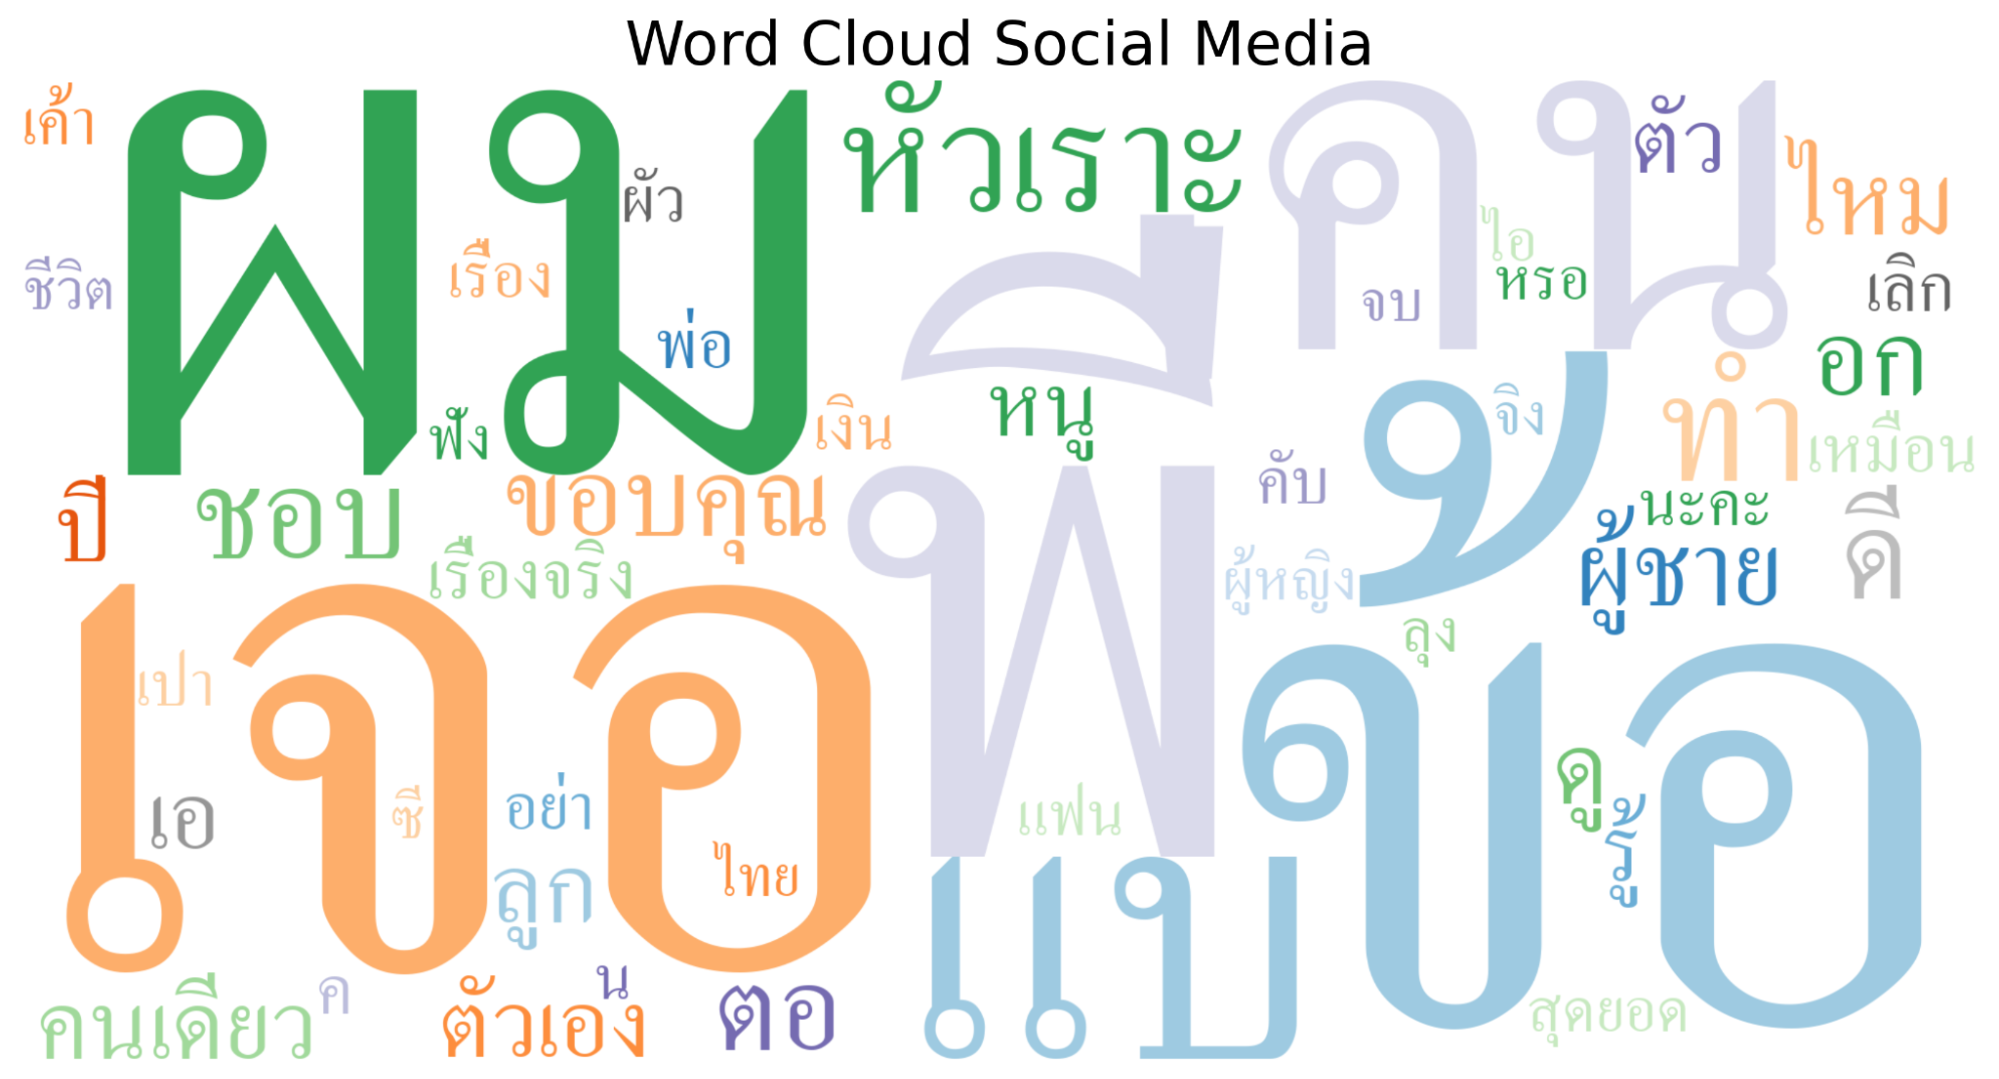
\includegraphics[width=0.8\linewidth]{assets/images/chapter4/image27.png}
\caption{Social Media Dataset Wordcloud (TikTok)}
\label{fig:tiktok-wordcloud}
\end{figure}

\subsection{Text Length Analysis}

\begin{table}[H]
\centering
\footnotesize
\caption{The Distribution of Token and Character Length Across Platforms}
\begin{tabular}{@{}lrrrrrrrrrrr@{}}
\toprule
Platform & Count & \shortstack{Mean\\Tokens} & \shortstack{Median\\Tokens} & Max & Min & \shortstack{Std\\Tokens} & \shortstack{Mean\\Chars} & \shortstack{Median\\Chars} & Max & Min & \shortstack{Std\\Chars} \\
\midrule
TikTok & 2,865 & 8.47 & 6 & 152 & 1 & 10.20 & 31.16 & 21 & 637 & 5 & 39.76 \\
Twitter & 18,079 & 25.58 & 18 & 495 & 1 & 21.43 & 97.80 & 69 & 2,285 & 5 & 84.99 \\
YouTube & 21,188 & 19.20 & 10 & 818 & 1 & 34.06 & 72.71 & 35 & 3,118 & 5 & 136.74 \\
\bottomrule
\end{tabular}
\end{table}

The distribution of token and character lengths across TikTok, Twitter, and YouTube comments. TikTok exhibits the shortest messages, with an average of 8.47 tokens and 31.16 characters, reflecting the platform's highly constrained interaction format and rapid comment style. Twitter displays a broader distribution, with a mean of 25.58 tokens and 97.80 characters, consistent with its moderate character limit (280 characters) and more conversational usage. YouTube comments are the longest on average (19.20 tokens, 72.71 characters), and show the largest variance, reaching up to 818 tokens and 3,118 characters, which aligns with YouTube's much more permissive comment length (up to 20,000 characters). The overall pattern indicates platform-dependent linguistic behavior that directly influences downstream NLP tasks, including tokenization efficiency, topic modeling stability, and annotation workload.



\begin{figure}[H]
\centering
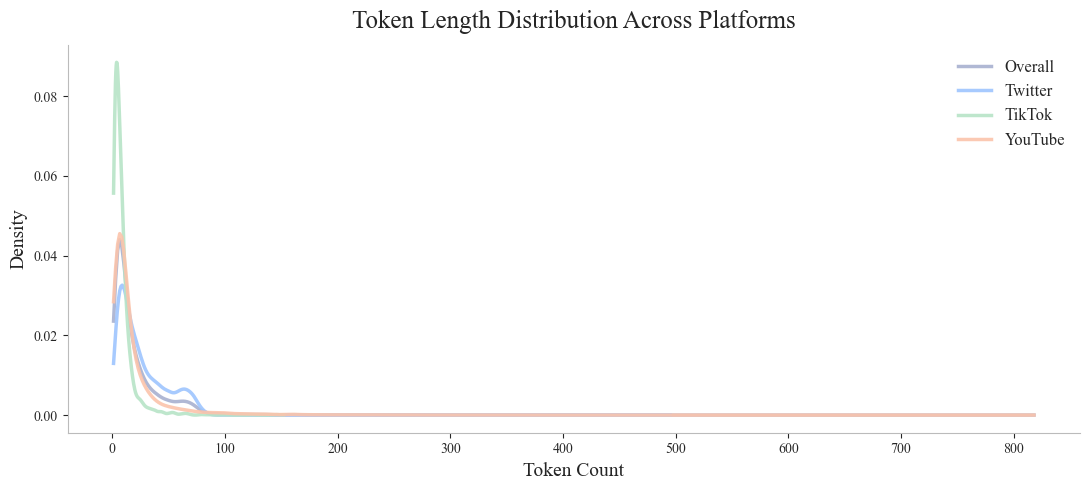
\includegraphics[width=0.8\linewidth]{assets/images/chapter4/image7.png}
\caption{Token Length Distribution Across Platform}
\label{fig:token-length-distribution-platform}
\end{figure}

The kernel density estimation (KDE) plot of token lengths in Figure~\ref{fig:token-length-distribution-platform} shows distinct platform-specific behavioral patterns influenced by character constraints and the interaction design of each site. TikTok exhibits the highest and narrowest peak, with comments concentrated within approximately 5--15 tokens, consistent with its 150-character limit and rapid, short-form interaction style. Twitter shows a slightly wider distribution, which reflects the platform's allowance for short opinions, replies, and hashtags. However, the majority of comments are below 100 tokens, suggesting that users rarely get close to the 280-character free-tier limit. In contrast, YouTube displays a significantly longer right-skewed tail that extends beyond 800 tokens. This is consistent with its lenient 20,000-character limit, which allows lengthy narratives, reviews, emotional reactions, and occasional spam.

Short text segments dominate the overall KDE distribution across platforms, despite the fact that these lengthy YouTube comments produce noticeable outliers. This suggests that most user-generated content, particularly that which contains bias or toxicity, tends to appear as short, reactive statements rather than lengthy discourse, a feature common to Thai social media communication patterns.

This indicates that conversations on social media, especially those that are toxic or gender-biased, are brief, impulsive, and reactive rather than long-form.

\subsection{BERTopic Without Embeddings}

In this experiment, we ran BERTopic without including any sentence-level embeddings, so the model generated topic clusters only using CountVectorizer (n-grams) and co-occurrence frequencies. The model only grouped documents based on surface-level token frequency because embeddings were disabled, which prevented it from capturing semantic relationships between sentences.

Since our dataset is scraped from multiple platforms (Twitter, TikTok, YouTube), the content naturally covers a wide range of themes, including love, comedy, gossip, MV discussions, gender references, and general Thai pop-culture vocabulary. In the absence of embeddings, BERTopic handles these lexical patterns as distinct clusters. The unigram result is shown in Figure~\ref{fig:unigram-bertopic-without-embedding-top-words} and Figure~\ref{fig:unigram-bertopic-without-embedding-intertopic-map}, the unigram-bigram result is shown in Figure~\ref{fig:unigram-bigram-bertopic-without-embedding-top-words} and Figure~\ref{fig:bigram-bertopic-without-embedding-intertopic-map}, and the unigram-trigram result is shown in Figure~\ref{fig:unigram-trigram-bertopic-without-embedding-top-words} and Figure~\ref{fig:trigram-bertopic-without-embedding-intertopic-map}.

\subsubsection{Unigram}

\begin{figure}[H]
\centering
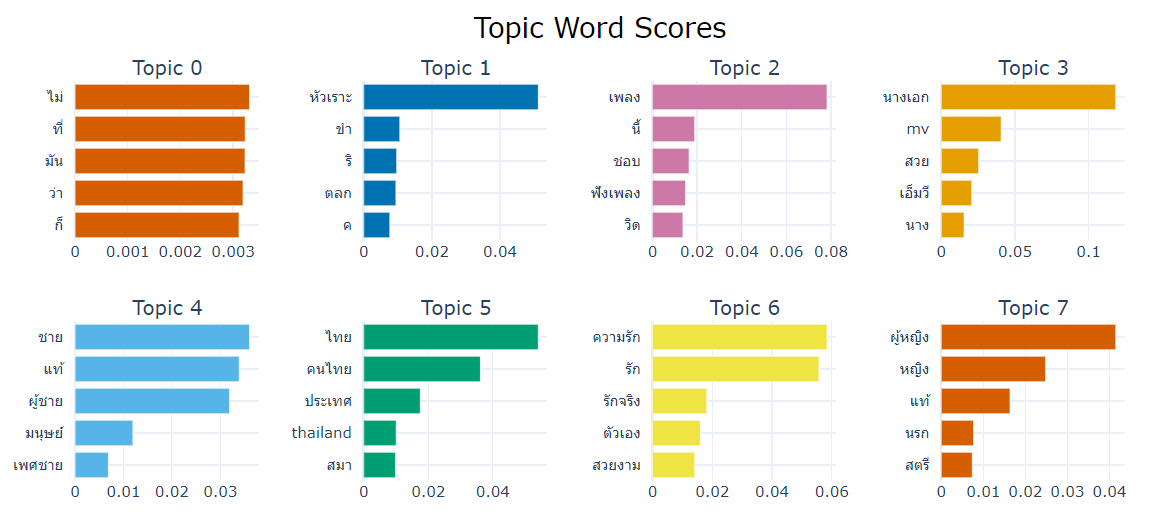
\includegraphics[width=0.8\linewidth]{assets/images/chapter4/image9.png}
\caption{Top 8 Topic Word Score of Unigram BERTopic without Embedding}
\label{fig:unigram-bertopic-without-embedding-top-words}
\end{figure}

\begin{figure}[H]
\centering
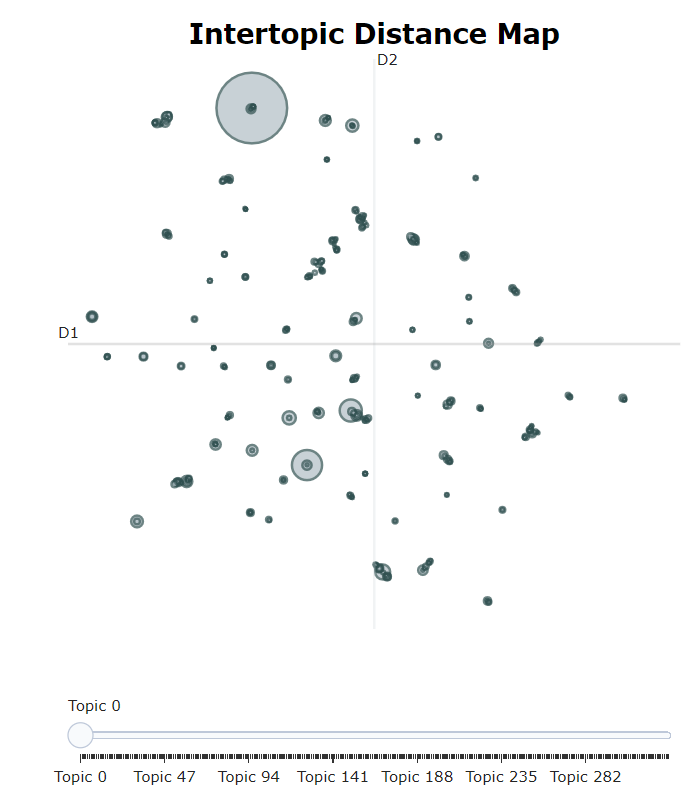
\includegraphics[width=0.8\linewidth]{assets/images/chapter4/image14.png}
\caption{Intertopic Distance Map of Unigram BERTopic without Embedding}
\label{fig:unigram-bertopic-without-embedding-intertopic-map}
\end{figure}

\clearpage
\subsubsection{Unigram-Bigram}

\begin{figure}[H]
\centering
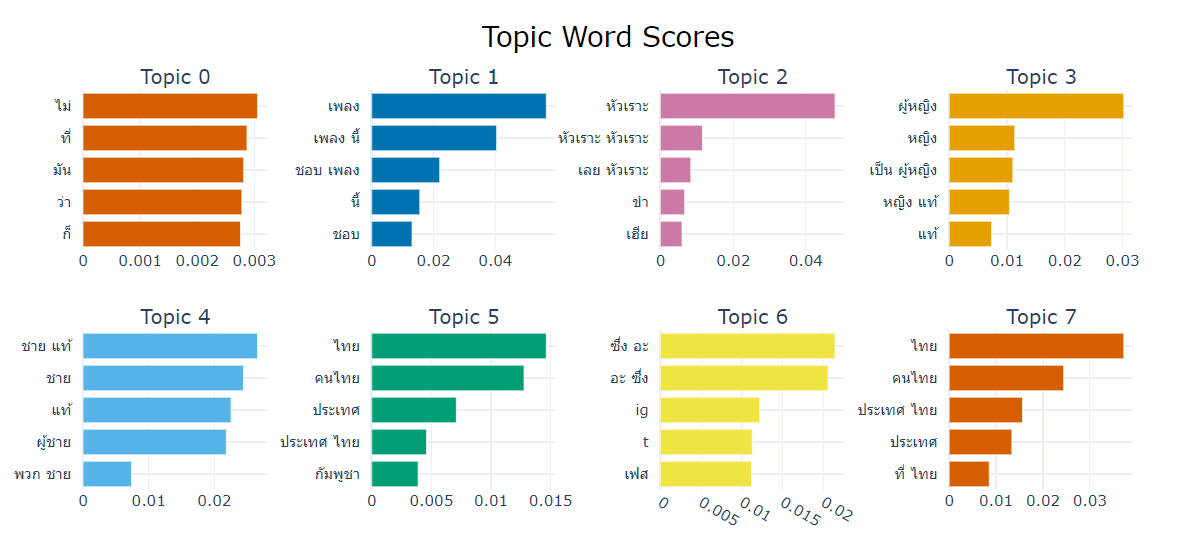
\includegraphics[width=0.75\linewidth]{assets/images/chapter4/image26.png}
\caption{Top 8 Topic Word Score of Unigram-Bigram BERTopic without Embedding}
\label{fig:unigram-bigram-bertopic-without-embedding-top-words}
\end{figure}

\begin{figure}[H]
\centering
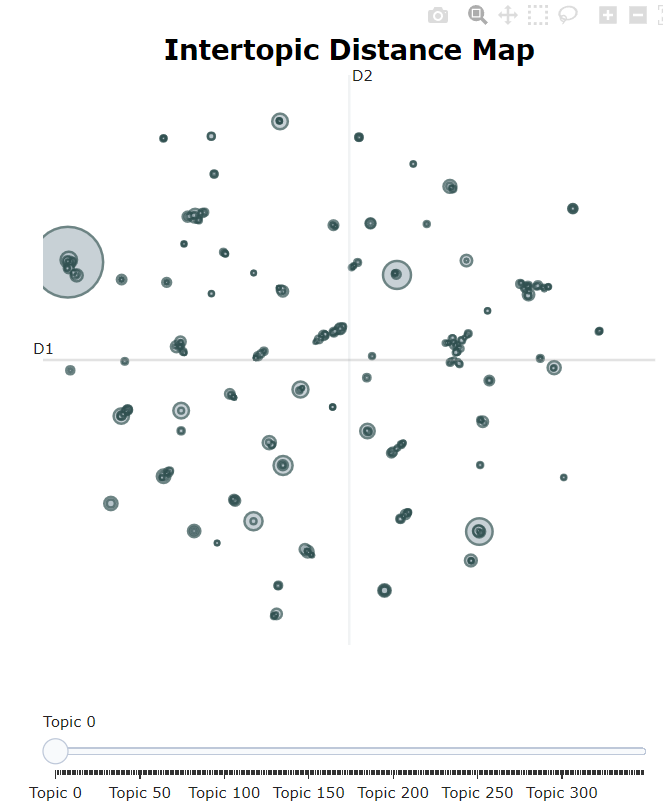
\includegraphics[width=0.75\linewidth]{assets/images/chapter4/image1.png}
\caption{Intertopic Distance Map of Bigram BERTopic without Embedding}
\label{fig:bigram-bertopic-without-embedding-intertopic-map}
\end{figure}

\clearpage
\subsubsection{unigram-trigrams}

\begin{figure}[H]
\centering
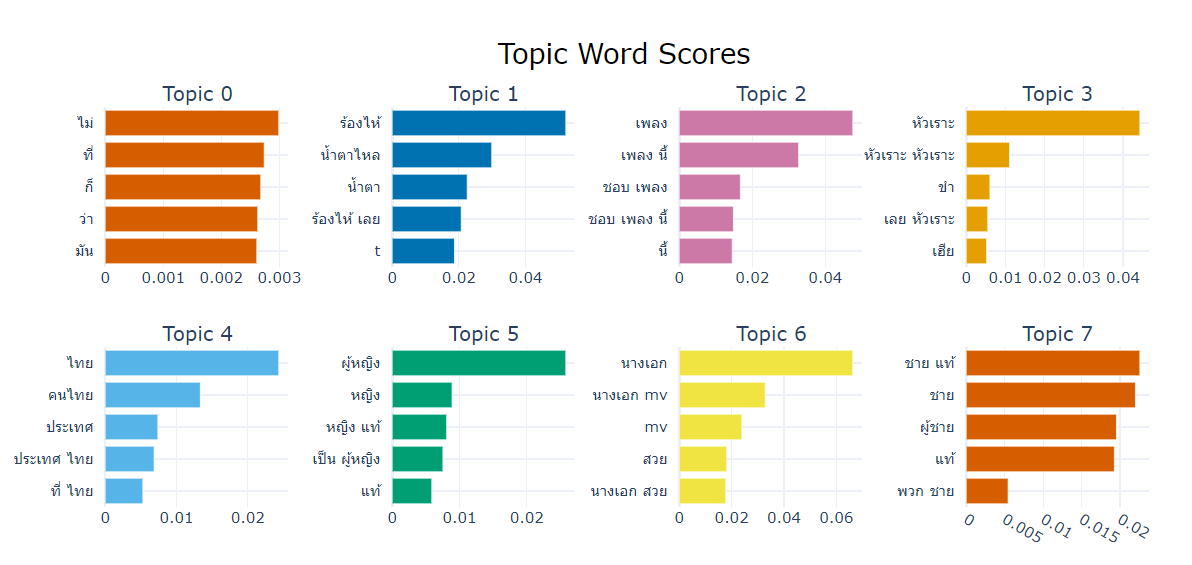
\includegraphics[width=0.75\linewidth]{assets/images/chapter4/image17.png}
\caption{Top 8 Topic Word Score of unigram-trigrams BERTopic without Embedding}
\label{fig:unigram-trigram-bertopic-without-embedding-top-words}
\end{figure}

\begin{figure}[H]
\centering
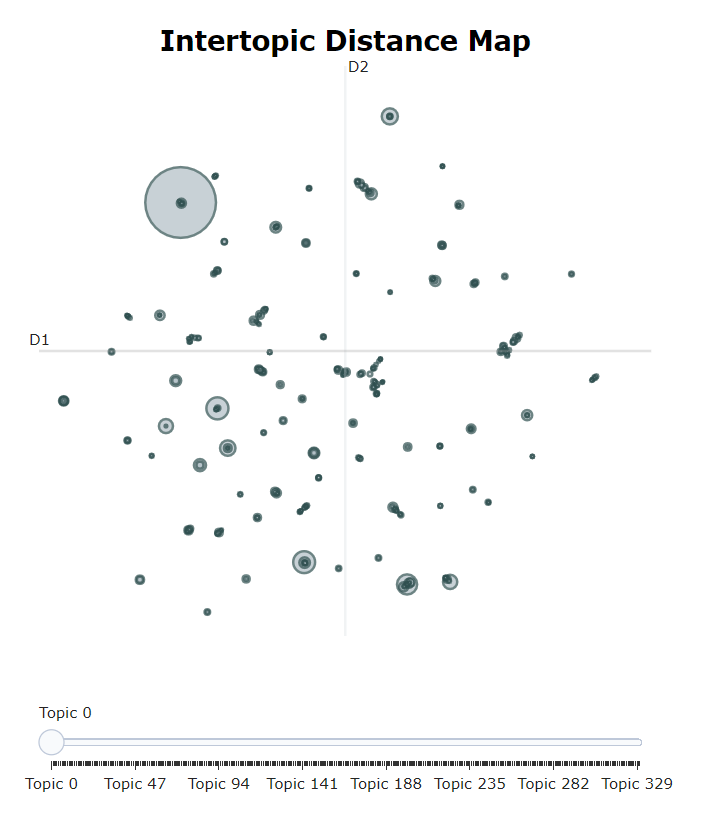
\includegraphics[width=0.75\linewidth]{assets/images/chapter4/image12.png}
\caption{Intertopic Distance Map of 3-grams BERTopic without Embedding}
\label{fig:trigram-bertopic-without-embedding-intertopic-map}
\end{figure}

\clearpage
\subsection{BERTopic With Embeddings}

\subsubsection{Topic Coherence Sweep Results}

\begin{table}[H]
\centering
\small
\caption{Topic Coherence Sweep Result Among Embedding Models}
\begin{tabular}{@{}lll@{}}
\toprule
\textbf{Embedding} & \textbf{N-gram} & \textbf{Coherence} \\
\midrule
bge-m3 & (1, 1) & 0.4080394417 \\
bge-m3 & (1, 2) & 0.5112899828 \\
bge-m3 & (2, 3) & 0.4544324325 \\
wangchan-simcse & (1, 1) & 0.4325159708 \\
wangchan-simcse & (1, 2) & 0.52032178 \\
wangchan-simcse & (2, 3) & 0.468718084 \\
nomic-v2 & (1, 1) & 0.4120271658 \\
nomic-v2 & (1, 2) & 0.5179071981 \\
nomic-v2 & (2, 3) & 0.4652337524 \\
\bottomrule
\end{tabular}
\end{table}

Results show that coherence consistently increases with larger n-grams, indicating that Thai gender-bias expressions often appear as multi-word constructions rather than isolated tokens. Among embedding models, Wangchan-simcse with (1,2) n-grams achieves the highest coherence, suggesting stronger semantic clustering of bias-related patterns.

Overall, the sweep indicates that multi-gram features are essential for capturing nuanced stereotypes and derogatory phrasing, and Wangchan-simcse provides the most coherent topic structure, making it suitable for downstream exploratory analysis and supporting span-level bias interpretation.

\subsubsection{Bge-m3}

The Bge-m3 topics in Figure~\ref{fig:bge-m3-bertopic-with-embedding-top-words} and Figure~\ref{fig:bge-m3-bertopic-with-embedding-intertopic-map} exhibit clear thematic clusters, capturing lexical patterns such as gendered insults, reference to physical appearance, and sexualized expressions.

\begin{figure}[H]
\centering
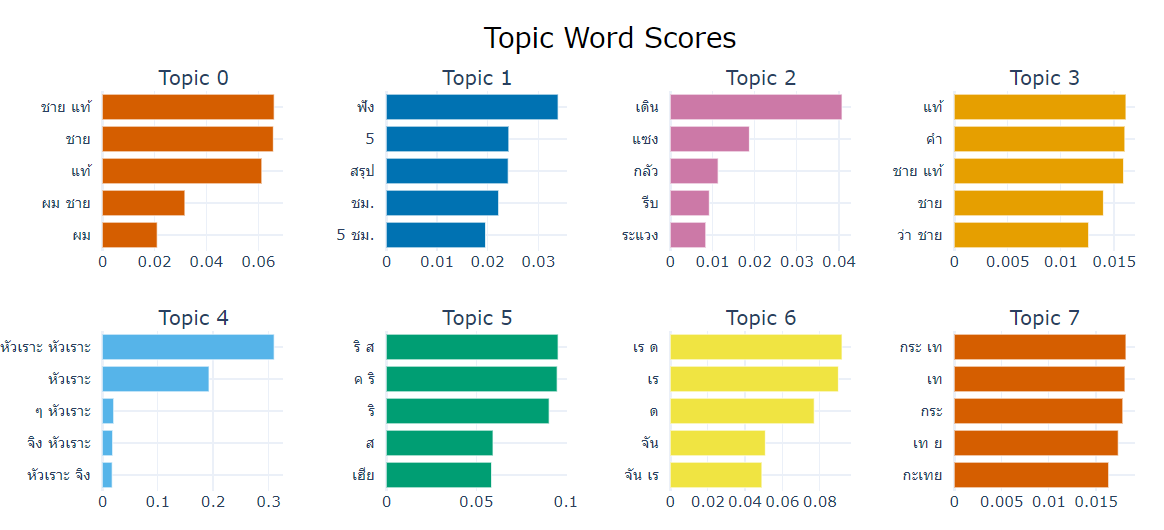
\includegraphics[width=0.8\linewidth]{assets/images/chapter4/image22.png}
\caption{Top 8 Topic Word Score of  (1, 2) gram  BERTopic with Embedding using Bge-m3}
\label{fig:bge-m3-bertopic-with-embedding-top-words}
\end{figure}

\begin{figure}[H]
\centering
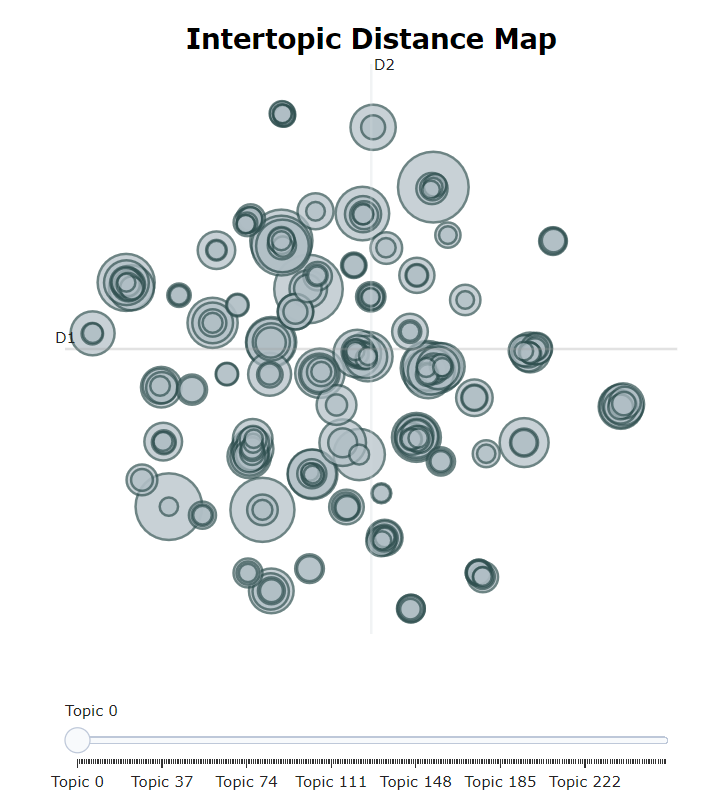
\includegraphics[width=0.8\linewidth]{assets/images/chapter4/image25.png}
\caption{Intertopic Distance Map of  (1, 2) gram  BERTopic with Embedding using Bge-m3}
\label{fig:bge-m3-bertopic-with-embedding-intertopic-map}
\end{figure}

This suggests that Bge-m3 can identify distinct thematic structures but may embed some semantically related abusive expressions within neighboring clusters, reflecting limitations in capturing fine-grained Thai social-media slang.

\subsubsection{Wangchan-simcse}

The Wangchan-simcse topics in Figure~\ref{fig:wangchan-simcse-bertopic-with-embedding-top-words} display improved lexical cohesion, with clearer grouping of gendered stereotypes, derogatory slang, and norm-violating expressions.

\begin{figure}[H]
\centering
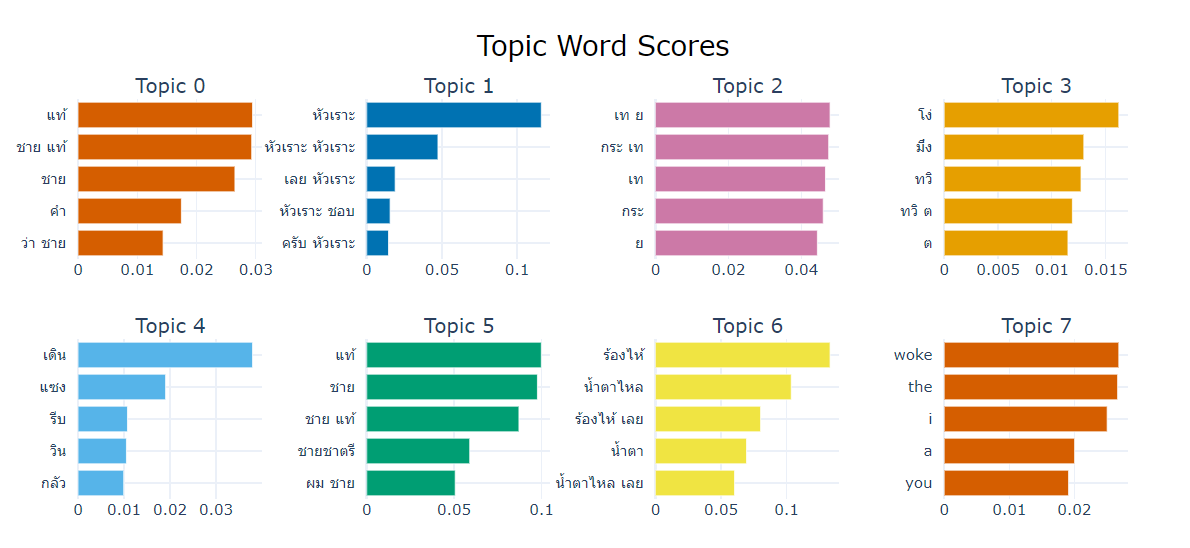
\includegraphics[width=0.8\linewidth]{assets/images/chapter4/image8.png}
\caption{Top 8 Topic Word Score of  (1, 2) gram  BERTopic with Embedding using Wangchan-simcse}
\label{fig:wangchan-simcse-bertopic-with-embedding-top-words}
\end{figure}



\begin{figure}[H]
\centering
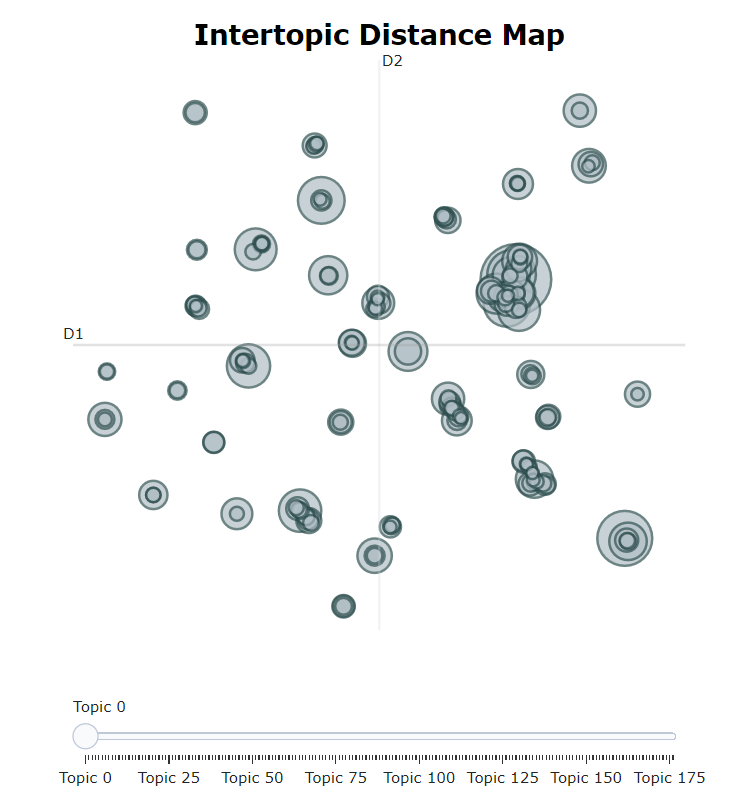
\includegraphics[width=0.8\linewidth]{assets/images/chapter4/image15.png}
\caption{Intertopic Distance Map of  (1, 2) gram  BERTopic with Embedding using Wangchan-simcse}
\label{fig:wangchan-simcse-intertopic-distance-map}
\end{figure}



The Intertopic Distance Map in Figure~\ref{fig:wangchan-simcse-intertopic-distance-map} reveals stronger cluster separation compared with Bge-m3. Topics are more compact, and overlapping regions are reduced, reflecting the higher coherence observed in the sweep experiments. This indicates that Wangchan-simcse captures Thai semantic similarity more effectively, especially in informal and bias-laden contexts.

\subsubsection{nomic-v2}

\begin{figure}[H]
\centering
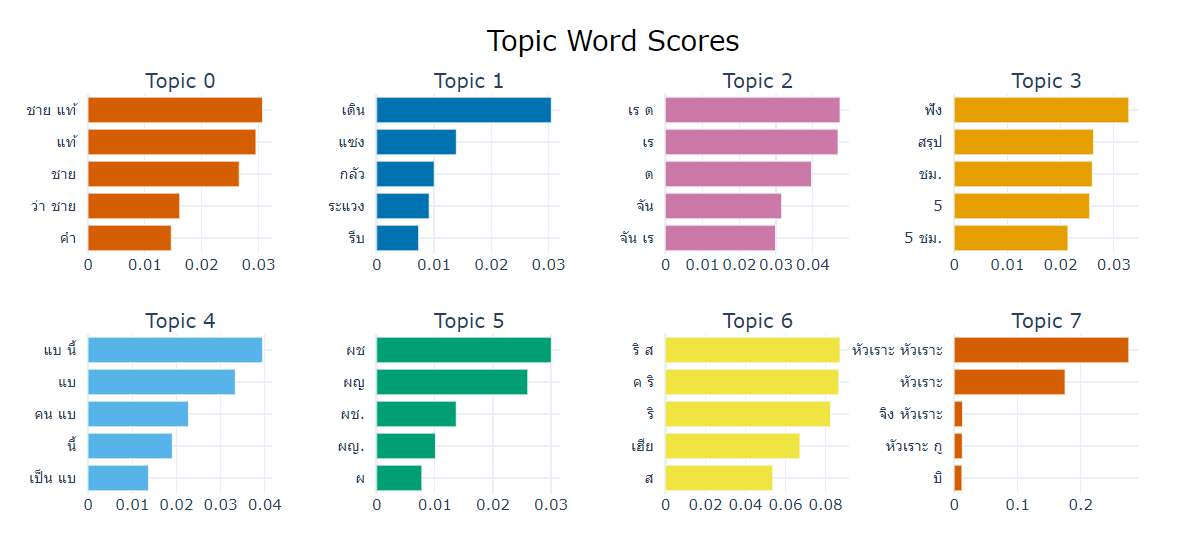
\includegraphics[width=0.8\linewidth]{assets/images/chapter4/image5.png}
\caption{Top 8 Topic Word Score of  (1, 2) gram  BERTopic with Embedding using nomic-v2}
\label{fig:nomic-v2-bertopic-with-embedding-top-words}
\end{figure}

\begin{figure}[H]
\centering
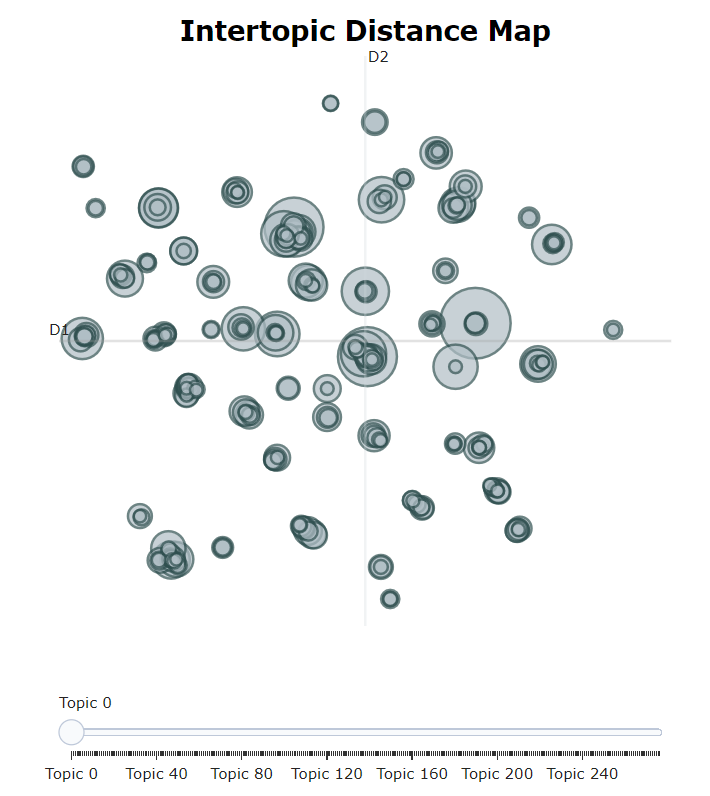
\includegraphics[width=0.8\linewidth]{assets/images/chapter4/image10.png}
\caption{Intertopic Distance Map of  (1, 2) gram  BERTopic with Embedding using nomic-v2}
\label{fig:nomic-v2-bertopic-with-embedding-intertopic-map}
\end{figure}

The nomic-v2 topic outputs in Figure~\ref{fig:nomic-v2-bertopic-with-embedding-top-words} and Figure~\ref{fig:nomic-v2-bertopic-with-embedding-intertopic-map} provide the third embedding-based comparison point. The coherence sweep reveals a consistent upward trend when moving from unigram to multi-gram features. For all embedding models, the (1,2) n-gram configuration yields the highest coherence. This indicates that Thai gender-biased expressions frequently consist of short multi-word constructions, including insults (``... หน้า... เหี้ย''), roles (``พวก... เฟมทวิต''), and sexualized phrasing, rather than isolated lexical tokens.

\subsubsection{BERTopic Topic Definition}

The three topic-definition files from Bge-m3, Wangchan-simcse, and nomic-v2 contain the full set of discovered topics, their token representations, and representative documents. These outputs were used to qualitatively compare how each embedding model structures Thai social media discourse related to gender bias. The comparison shows clear differences across the models in terms of topic granularity, noise reduction, semantic purity, and sensitivity to Thai social media slang.

\begin{itemize}
\item \textbf{Overall Topic Structure and Noise Proportion}\\
The first major difference concerns the number of generated topics and the size of the noise cluster, represented as Topic -1. As shown in Table X, Wangchan-simcse produced the fewest distinct topics, with 178 topics, suggesting stronger semantic grouping and better ability to merge related expressions into coherent themes. In contrast, Bge-m3 produced 259 topics, while nomic-v2 produced 278 topics, indicating a tendency toward more fragmented topic structures or micro-clusters. All three models produced a large Topic -1 cluster, but the interpretation differs by model. For Bge-m3 and nomic-v2, the noise cluster appears to reflect weaker Thai semantic alignment and greater ambiguity in embedding informal Thai expressions. For Wangchan-simcse, the noise cluster is large because similar slang or repetitive expressions are grouped tightly into clearer topics, leaving the remaining items as diverse residual content that does not fit well into the main clusters.
\end{itemize}

\begin{table}[H]
\centering
\small
\caption{Topic Structure and Noise Proportion Across Embedding Models}
\begin{tabularx}{\textwidth}{@{}l l l >{\raggedright\arraybackslash}X@{}}
\toprule
\textbf{Model} & \textbf{Total Topics} & \textbf{Topic --1 Count} & \textbf{Interpretation} \\
\midrule
bge-m3 & 259 topics & 21,700 noise docs & High noise: weaker Thai representation \\
Wangchan-simcse & 178 topics & 26,409 noise docs & Fewer topics: stronger clustering, but large noise due to strict semantic filtering \\
nomic-v2 & 278 topics & 19,133 noise docs & Many micro-clusters: over-segmentation \\
\bottomrule
\end{tabularx}
\end{table}

\begin{itemize}
\item \textbf{Dominant Themes Across Embeddings}\\
Across the three embedding models, several major themes of gender-biased discourse were consistently recovered. These include appearance-based insults, such as ``หน้า... เหี้ย'', ``อุบาทว์'', and ``น่ารังเกียจ''; sexualized language and harassment; gender-normative judgments, such as ``เป็นผู้ชายต้อง...'' and ``ผู้หญิงที่ดีต้อง...''; slurs and identity-based labels, such as ``กระเทย'', ``ตุ๊ด'', and ``ผู้ชายแท้''; and relationship stereotypes, such as ``ผู้หญิงแบบนี้ควรโดน...'' and ``ผู้ชายดีๆไม่มีหรอก''. The recurrence of these themes across all three models suggests that the collected corpus contains multiple forms of gender-related discourse, ranging from direct insults and sexualized expressions to stereotypes and identity-based labels.

\item \textbf{Qualitative Characteristics by Embedding Model}\\
Although all three models recovered similar broad themes, they differed in how clearly and consistently they organized these themes. Bge-m3 produced 259 topics, many of which appeared as micro-clusters. Its topic names showed overlap among related abusive expressions; for example, terms such as ``ชายแท้'', ``ผมชาย'', and ``แท้ชาย'' appeared across multiple clusters. This suggests that Bge-m3 can capture general semantic similarity, but it does not always merge related Thai gendered expressions into a single coherent topic. Some clusters also contained mixed semantic signals, such as combining role-based comments with appearance-based insults. Representative documents showed looser thematic boundaries, indicating that Bge-m3 struggles with Thai slang and code-switched expressions. As a result, the model produced fragmented topics and moderate noise.

Wangchan-simcse produced the fewest clusters, with 178 topics, which indicates stronger semantic cohesion. Its topics were clearer, more compact, and more culturally aligned than the other embedding models. In particular, Wangchan-simcse grouped together themes around LGBTQ+ references, such as ``เทย'' and ``กระเทย''; gender-norm statements; insults referencing intelligence or morality; and harassment-related content. Topic labels also showed higher lexical consistency, including groups such as ``หัวเราะ'', ``ด่า'', ``คำว่า ชาย'', and ``ทวิ ต''. The representative documents were more cleanly separated, with less contamination between unrelated stereotypes or abusive expressions. Overall, Wangchan-simcse exhibited the strongest Thai semantic competence and provided the most interpretable and coherent topic structure, confirming the quantitative coherence results from the earlier sweep.

Nomic-v2 produced 278 topics, the highest number among the three models. This suggests that it often created overly fine-grained clusters, resulting in many narrowly defined topics. Some of these topics successfully captured multilingual or code-switched expressions, showing that nomic-v2 can represent general multilingual semantic patterns. However, many clusters revolved around common functional expressions, such as ``ได้'', ``มี'', and ``ไม่'', which reduced interpretability because these words do not necessarily represent meaningful gender-bias themes. Therefore, nomic-v2 achieved reasonable general semantic grouping but lacked Thai-specific contextual depth. Its output was more interpretable than Bge-m3 in some multilingual cases, but less coherent and culturally precise than Wangchan-simcse for Thai gender-bias discourse.

\item \textbf{Cross-Model Comparison}\\
In terms of topic granularity, Wangchan-simcse produced the most balanced structure. Its clusters were fewer but more semantically meaningful, suggesting that it was able to group related expressions without excessive fragmentation. Bge-m3 and nomic-v2 generated more topics, but many of these appeared as micro-clusters or overlapping topics. This indicates that they separate expressions more finely, but often at the cost of thematic cohesion.

In terms of topic purity, Wangchan-simcse produced the clearest and most internally consistent topics. Its clusters were culturally coherent and showed less mixing between unrelated forms of bias. Bge-m3 had lower topic purity because it frequently grouped unrelated or only loosely related terms within the same topic. Nomic-v2 performed between the two models: it formed some meaningful clusters, especially around multilingual expressions, but did not reach the precision of Wangchan-simcse for Thai-specific gender-bias themes.

In terms of sensitivity to Thai social media slang, Wangchan-simcse again performed strongest. It showed a better ability to capture Thai slang, sarcasm, LGBTQ+ references, and culturally embedded expressions. This likely reflects its specialization in Thai language representations. Bge-m3 often failed to separate such expressions appropriately, leading to misclustered or overlapping topics. Nomic-v2 showed partial understanding of slang and code-switching, but did not consistently organize these expressions into coherent thematic groups.

The models also differed in their noise cluster behavior. All embedding models produced a large Topic -1 cluster, but the reasons appear different. For Bge-m3, the noise cluster likely reflects limited specialization in Thai, which leads to weak separation of heterogeneous content. For Wangchan-simcse, the noise cluster mainly contains residual items that do not fit into its otherwise well-defined topics. For nomic-v2, the noise is likely caused by its general-purpose multilingual embeddings, which are not directly tuned for Thai linguistic nuance.

Overall, the topic-definition results demonstrate that embedding choice strongly influences the semantic structure of discovered topics. Wangchan-simcse produced the most coherent, interpretable, and culturally aligned topic taxonomy. In contrast, Bge-m3 and nomic-v2 showed more fragmentation and lower topic purity. These findings align with the coherence sweep results and reinforce that Thai-trained embeddings are important for modeling gender-biased discourse in Thai social media.
\end{itemize}

\subsection{Toxicity and Safety Distribution Analysis}

The toxicity and safety pseudo-labeling results were analyzed to understand harmful-language patterns across platforms. CREST and one-for-all-toxicity-v3 produced complementary views of the dataset. CREST captured broader unsafe or policy-relevant content, while one-for-all-toxicity-v3 was more sensitive to social-media toxicity, including aggressive or hostile language.

\begin{figure}[H]
\centering
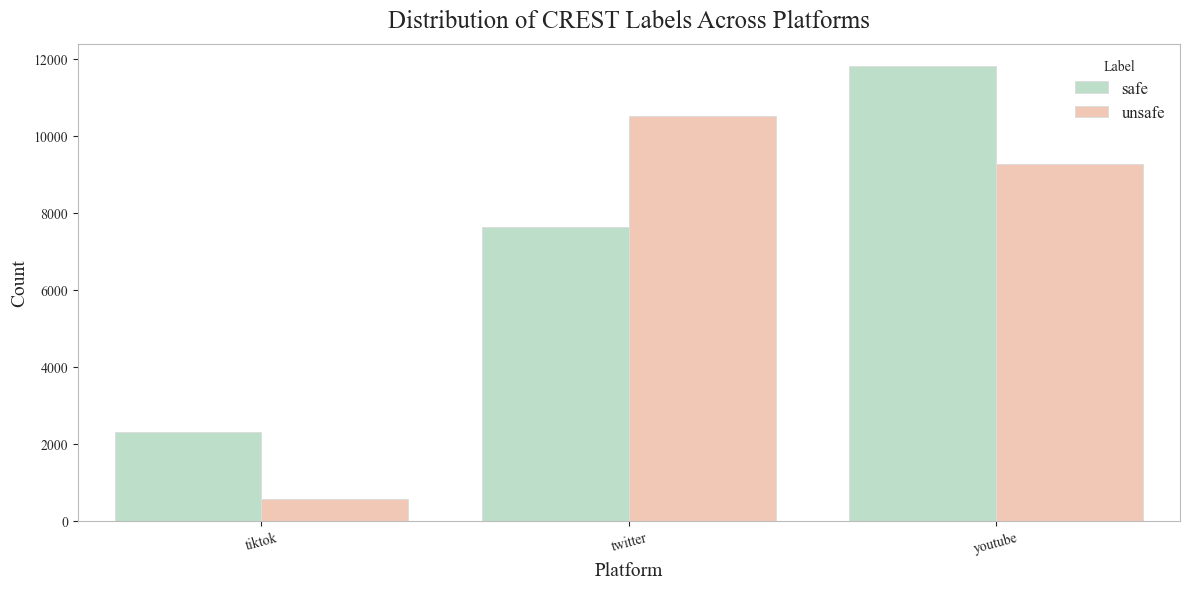
\includegraphics[width=0.8\linewidth]{assets/images/chapter4/image18.png}
\caption{Distribution of CREST Labels Across Platforms}
\label{fig:crest-label-distribution-platforms}
\end{figure}

Figure~\ref{fig:crest-label-distribution-platforms} shows the distribution of CREST labels across platforms. Twitter/X shows the highest proportion of unsafe content, which may reflect the adversarial and fast-moving nature of conversations on the platform. YouTube has a lower unsafe proportion than Twitter/X but contributes a large absolute number of unsafe comments because of its larger comment volume and longer discussion format. TikTok contains the lowest proportion of unsafe content, which may be related to the shorter and more reactive nature of its comments.

\begin{figure}[H]
\centering
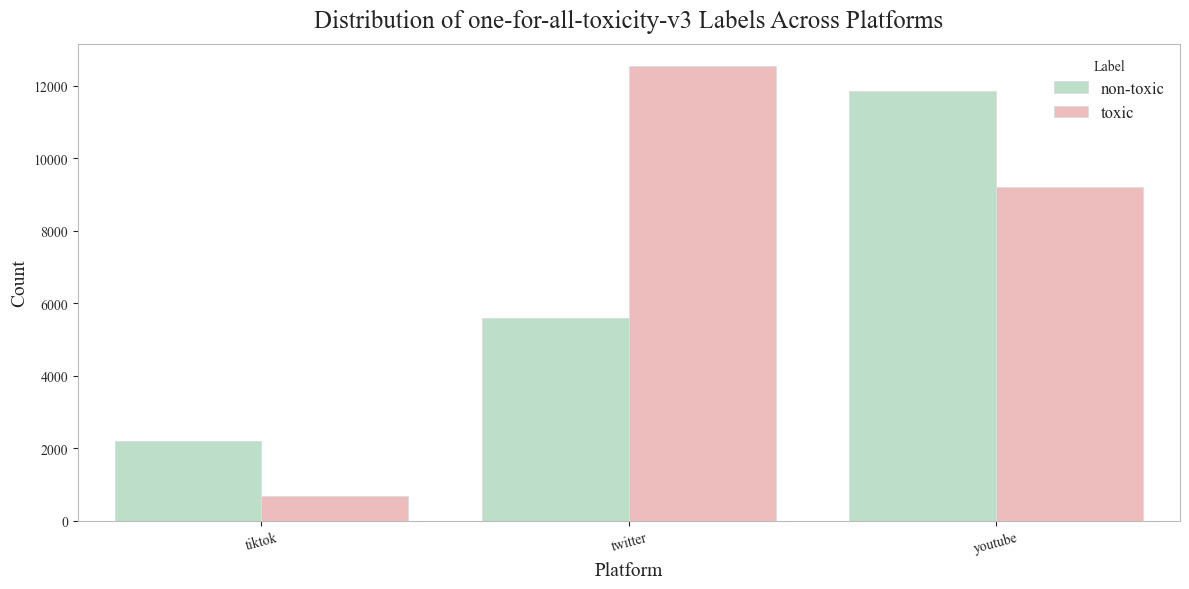
\includegraphics[width=0.8\linewidth]{assets/images/chapter4/image23.png}
\caption{Distribution of one-for-all-toxicity-v3 Labels Across Platforms}
\label{fig:toxicity-label-distribution-platforms}
\end{figure}

Figure~\ref{fig:toxicity-label-distribution-platforms} presents the toxicity distribution from one-for-all-toxicity-v3. The results show a similar overall trend, with Twitter/X containing the strongest toxicity signal, YouTube showing a moderate level, and TikTok containing relatively few toxic comments. These patterns suggest that platform style affects the type of harmful language observed in the corpus.

\subsubsection{Agreement Between Toxicity and Safety Models}

\begin{figure}[H]
\centering
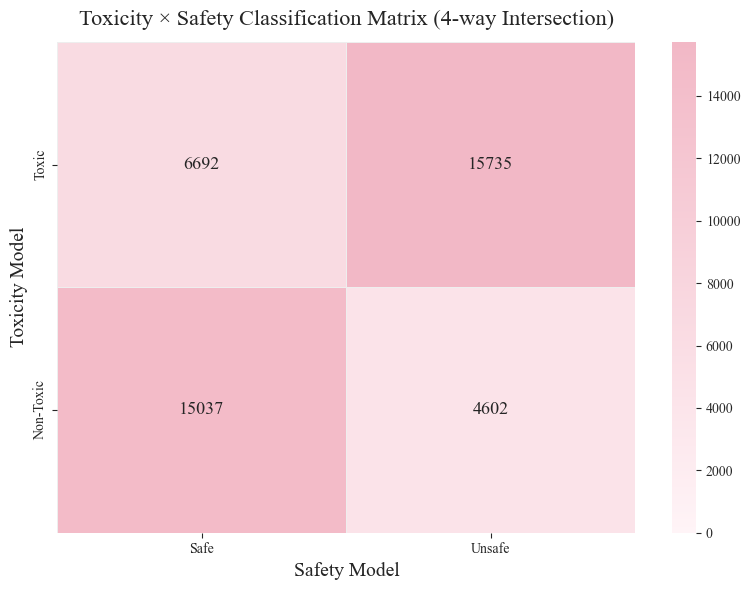
\includegraphics[width=0.8\linewidth]{assets/images/chapter4/image13.png}
\caption{Classification matrix of the result from pseudo-labeling}
\label{fig:pseudo-labeling-agreement-matrix}
\end{figure}

Figure~\ref{fig:pseudo-labeling-agreement-matrix} shows the agreement matrix between the CREST safety classifier and the one-for-all-toxicity-v3 model. The purpose of this comparison was to understand how different harmful-language classifiers characterize the collected corpus. Although this process was not used as the final filtering method for human annotation, it provided useful insight into the relationship between general toxicity, unsafe language, and possible gender-bias expressions.

When both models classify a sentence as toxic or unsafe, the sentence is more likely to contain harmful, aggressive, or sensitive language. These cases may overlap with gender-bias expressions, especially when the text includes harassment, sexualized language, gendered insults, or degrading descriptions. However, toxicity and gender bias are not the same concept, so these outputs were treated only as exploratory signals rather than direct gender-bias labels.

The disagreement cases are also informative. Sentences classified as toxic but safe often contain hostile or emotionally charged language without clear policy-level harm. In contrast, sentences classified as non-toxic but unsafe may contain more implicit or contextual harms, such as gender-role stereotypes, normative claims, or culturally embedded discriminatory expressions. This suggests that the two models capture different aspects of harmful language: one-for-all-toxicity-v3 is more sensitive to overt aggression, while CREST is more sensitive to broader unsafe or policy-relevant content.

Overall, the agreement analysis shows that toxicity and safety pseudo-labels can provide useful supporting insight during corpus exploration. However, because this process overlaps with topic modeling and may reduce the available annotation pool if used as a strict filter, it was not retained as the final candidate-selection method. Topic modeling was used instead to select gender- and SOGI-related topics more directly.

\section{Data Annotation}

\subsection{Dataset Distribution After Human Annotation}

\begin{figure}[H]
\centering
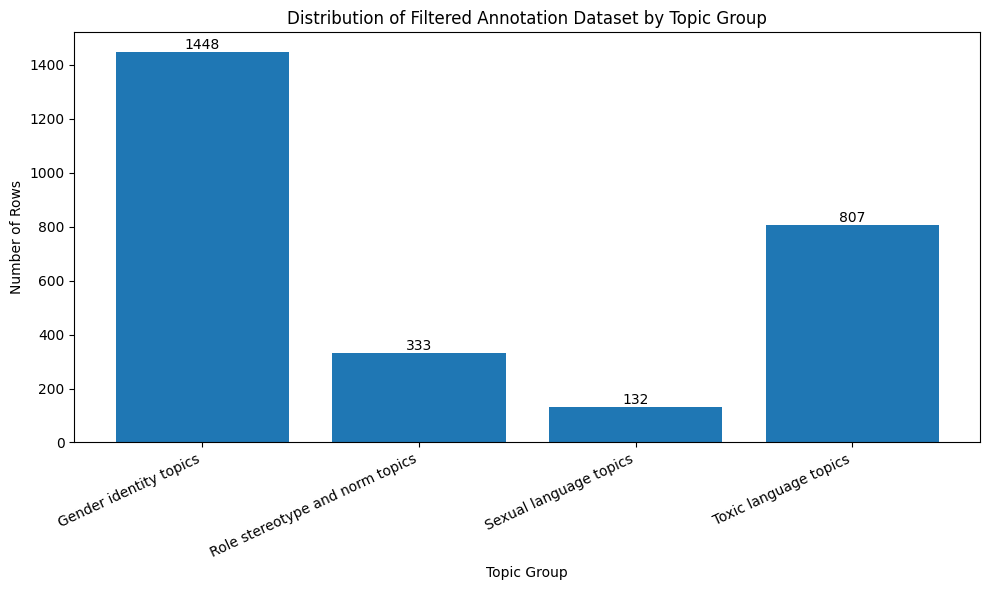
\includegraphics[width=0.8\linewidth]{assets/images/chapter4/image3.png}
\caption{Distribution of Filtered Annotation Dataset by Topic Group}
\label{fig:filtered-annotation-dataset-topic-group-distribution}
\end{figure}

Figure~\ref{fig:filtered-annotation-dataset-topic-group-distribution} shows that the initial data collection process produced 52,055 unique text records from YouTube, Twitter/X, and TikTok after deduplication. However, not all collected records were directly used for human annotation. To prioritize data that was more likely to contain gender- or SOGI-related bias, topic modeling was applied using Wangchan-SimCSE. After filtering for topics related to gender bias, the annotation dataset was reduced to 2,720 rows. These selected rows came from several relevant topic groups, including gender identity topics with 1,448 rows, role stereotype and norm topics with 333 rows, sexual language topics with 132 rows, and toxic language topics with 807 rows. This filtering step helped reduce irrelevant content and allowed annotators to focus on higher-signal samples.

\begin{figure}[H]
\centering
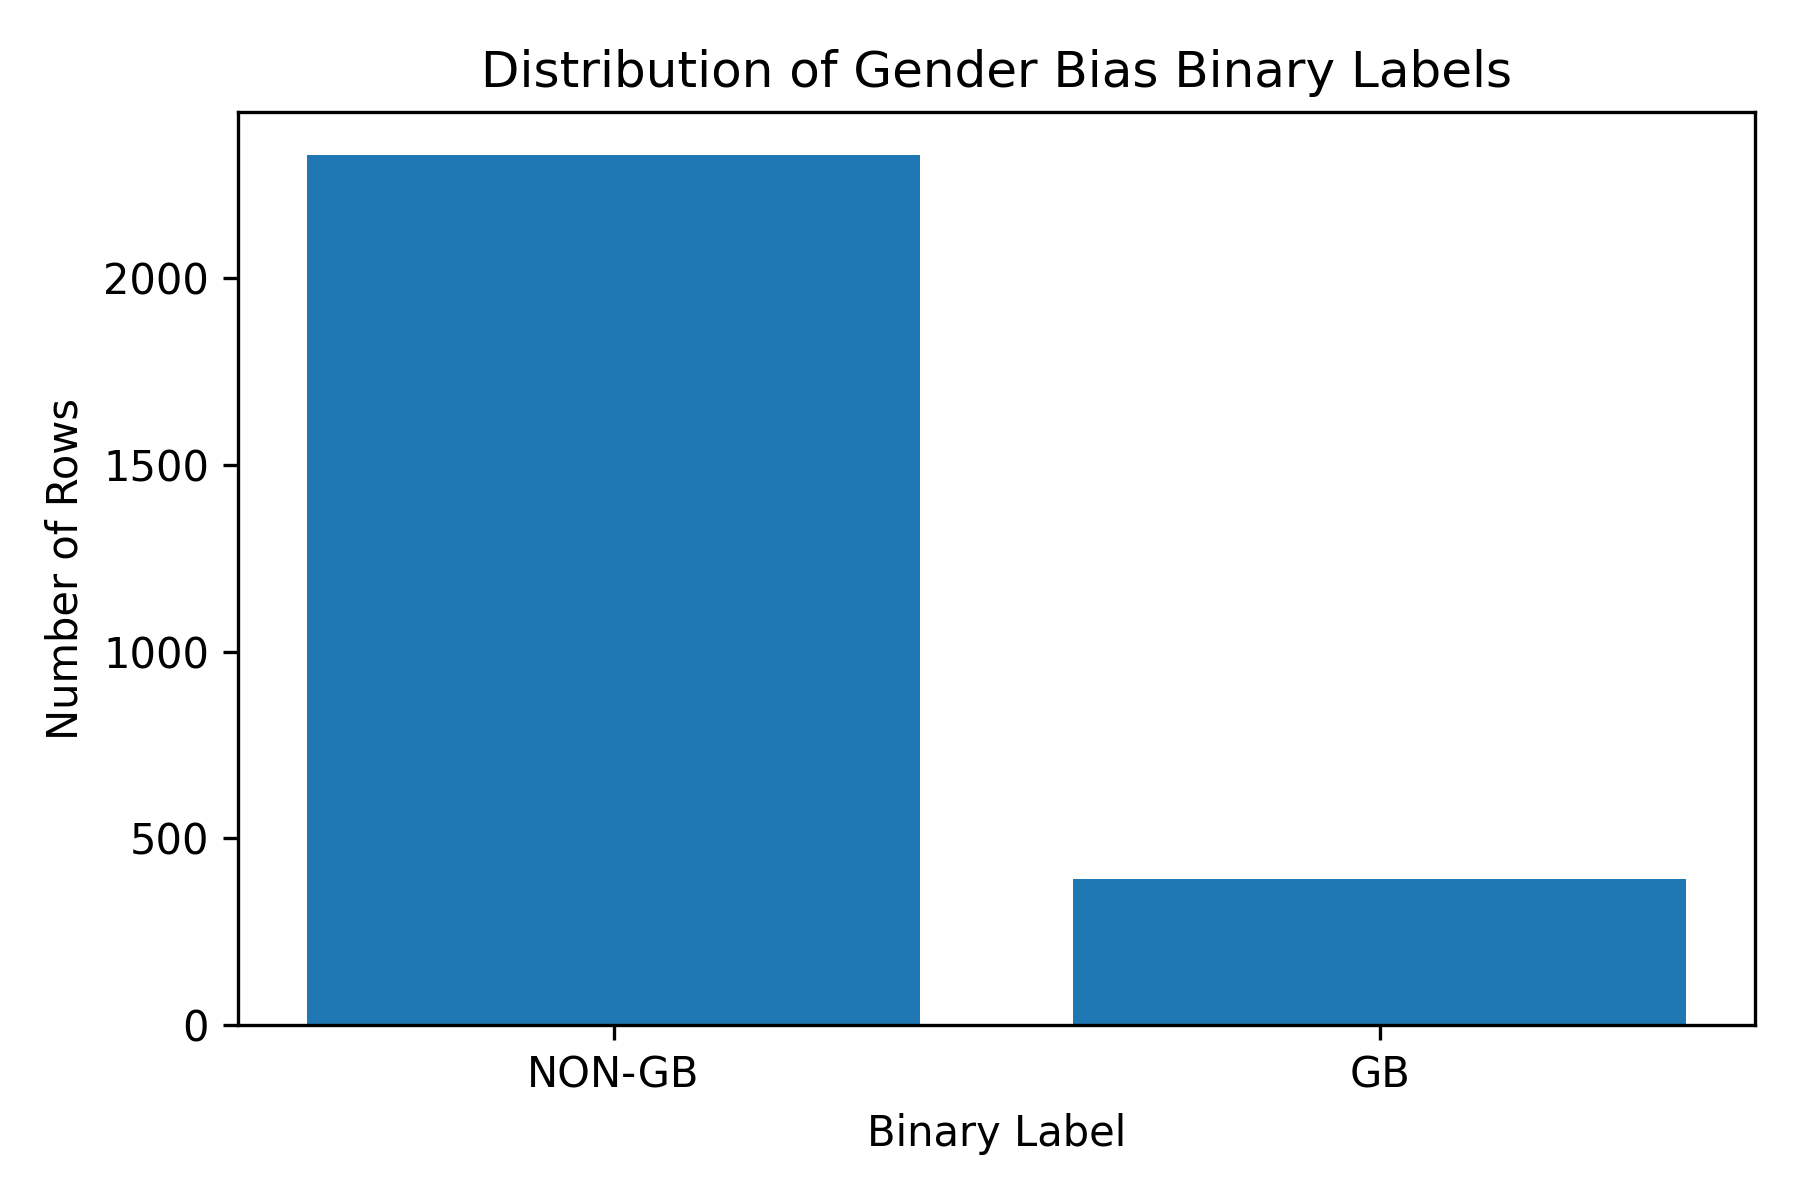
\includegraphics[width=0.8\linewidth]{assets/images/chapter4/image24.png}
\caption{Distribution of Gender Bias Binary Labels}
\label{fig:gender-bias-binary-label-distribution}
\end{figure}

After human annotation using the web annotator tool, the dataset contained 2,720 annotated rows in total. The binary label distribution in Figure~\ref{fig:gender-bias-binary-label-distribution} shows a clear imbalance between NON-GB and GB samples. There are 2,328 NON-GB rows, accounting for 85.59\% of the dataset, while only 392 rows are labeled as GB, accounting for 14.41\%. This indicates that most collected social media text does not contain gender bias according to the annotation guideline, while gender-biased content appears much less frequently.

However, this distribution should be interpreted with caution because some social media posts depend heavily on surrounding context. For example, a reply or mention may appear neutral when viewed alone but may carry gender-biased meaning when interpreted together with the original tweet, video, or comment thread. Since the annotation process mainly focuses on the extracted sentence or comment text, some context-dependent gender bias may be labeled as NON-GB due to the lack of surrounding post context. This limitation may partly contribute to the high proportion of NON-GB samples in the annotated dataset.

\begin{figure}[H]
\centering
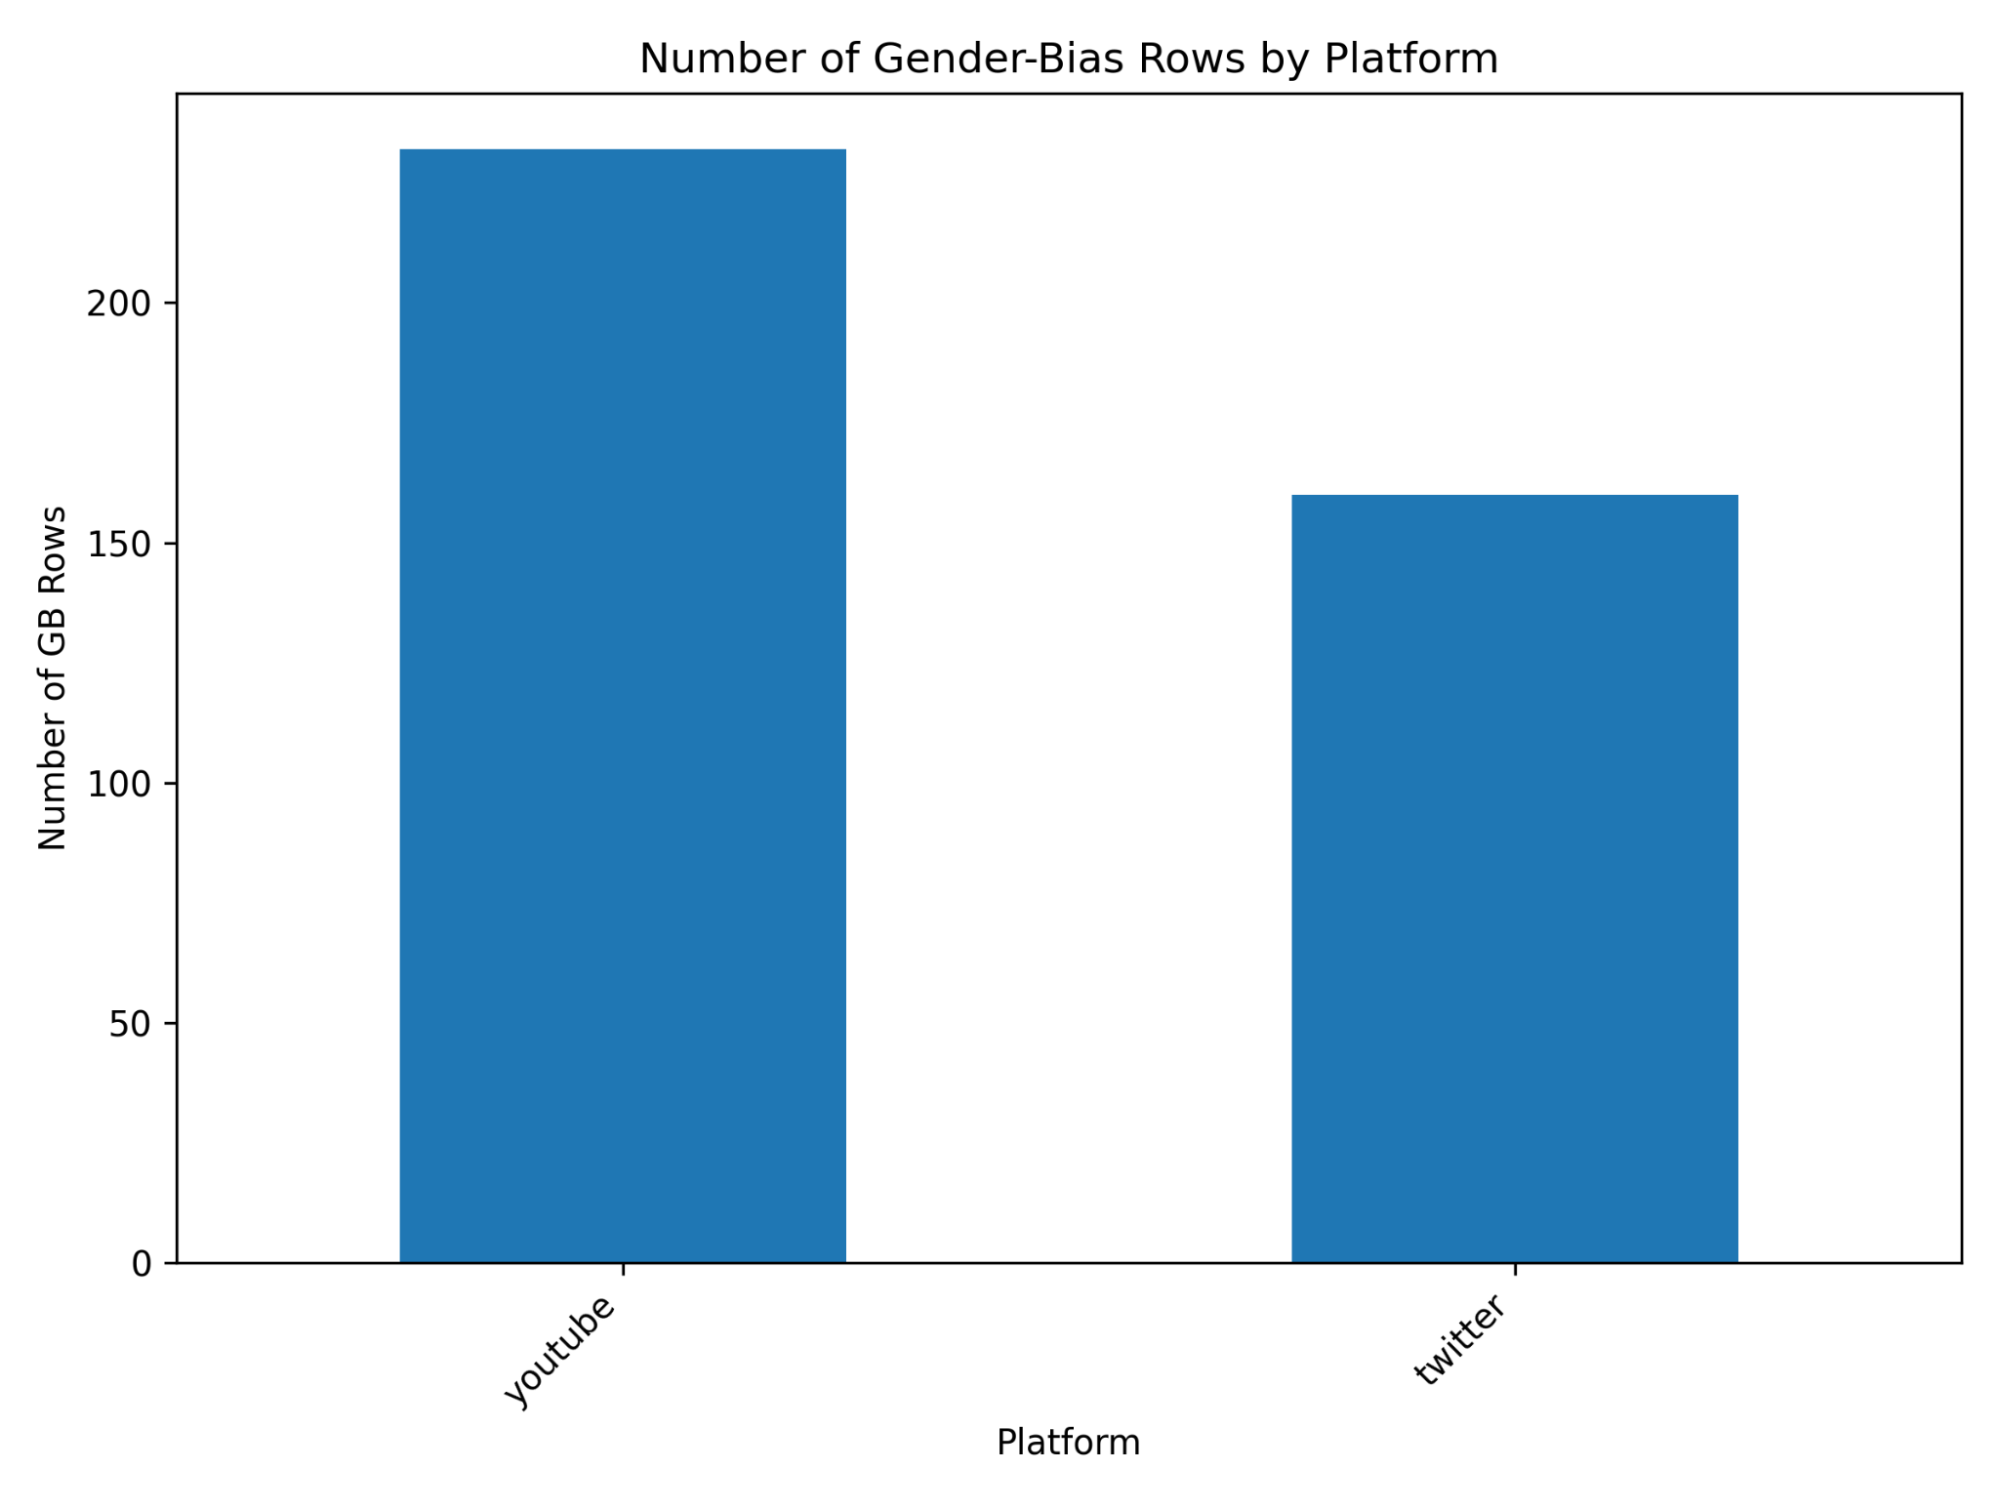
\includegraphics[width=0.8\linewidth]{assets/images/chapter4/image16.png}
\caption{Distribution of GB Types}
\label{fig:gb-platform-distribution}
\end{figure}

After identifying the GB rows, the platform distribution of gender-biased samples was also examined in Figure~\ref{fig:gb-platform-distribution}. The results show that GB samples came from only two platforms in the annotated subset: YouTube and Twitter/X. YouTube contributed the largest number of GB rows, with 232 rows, while Twitter/X contributed 160 rows. TikTok did not appear in the GB distribution. One possible reason is the nature of TikTok comments, which are often short, reactive, and highly dependent on the video context. Without the surrounding video content or full comment thread, many TikTok comments may not provide enough textual evidence to be labeled as GB. In contrast, YouTube and Twitter/X often contain longer comments, replies, or discussions, giving annotators more context to identify gender-biased expressions.

\begin{figure}[H]
\centering
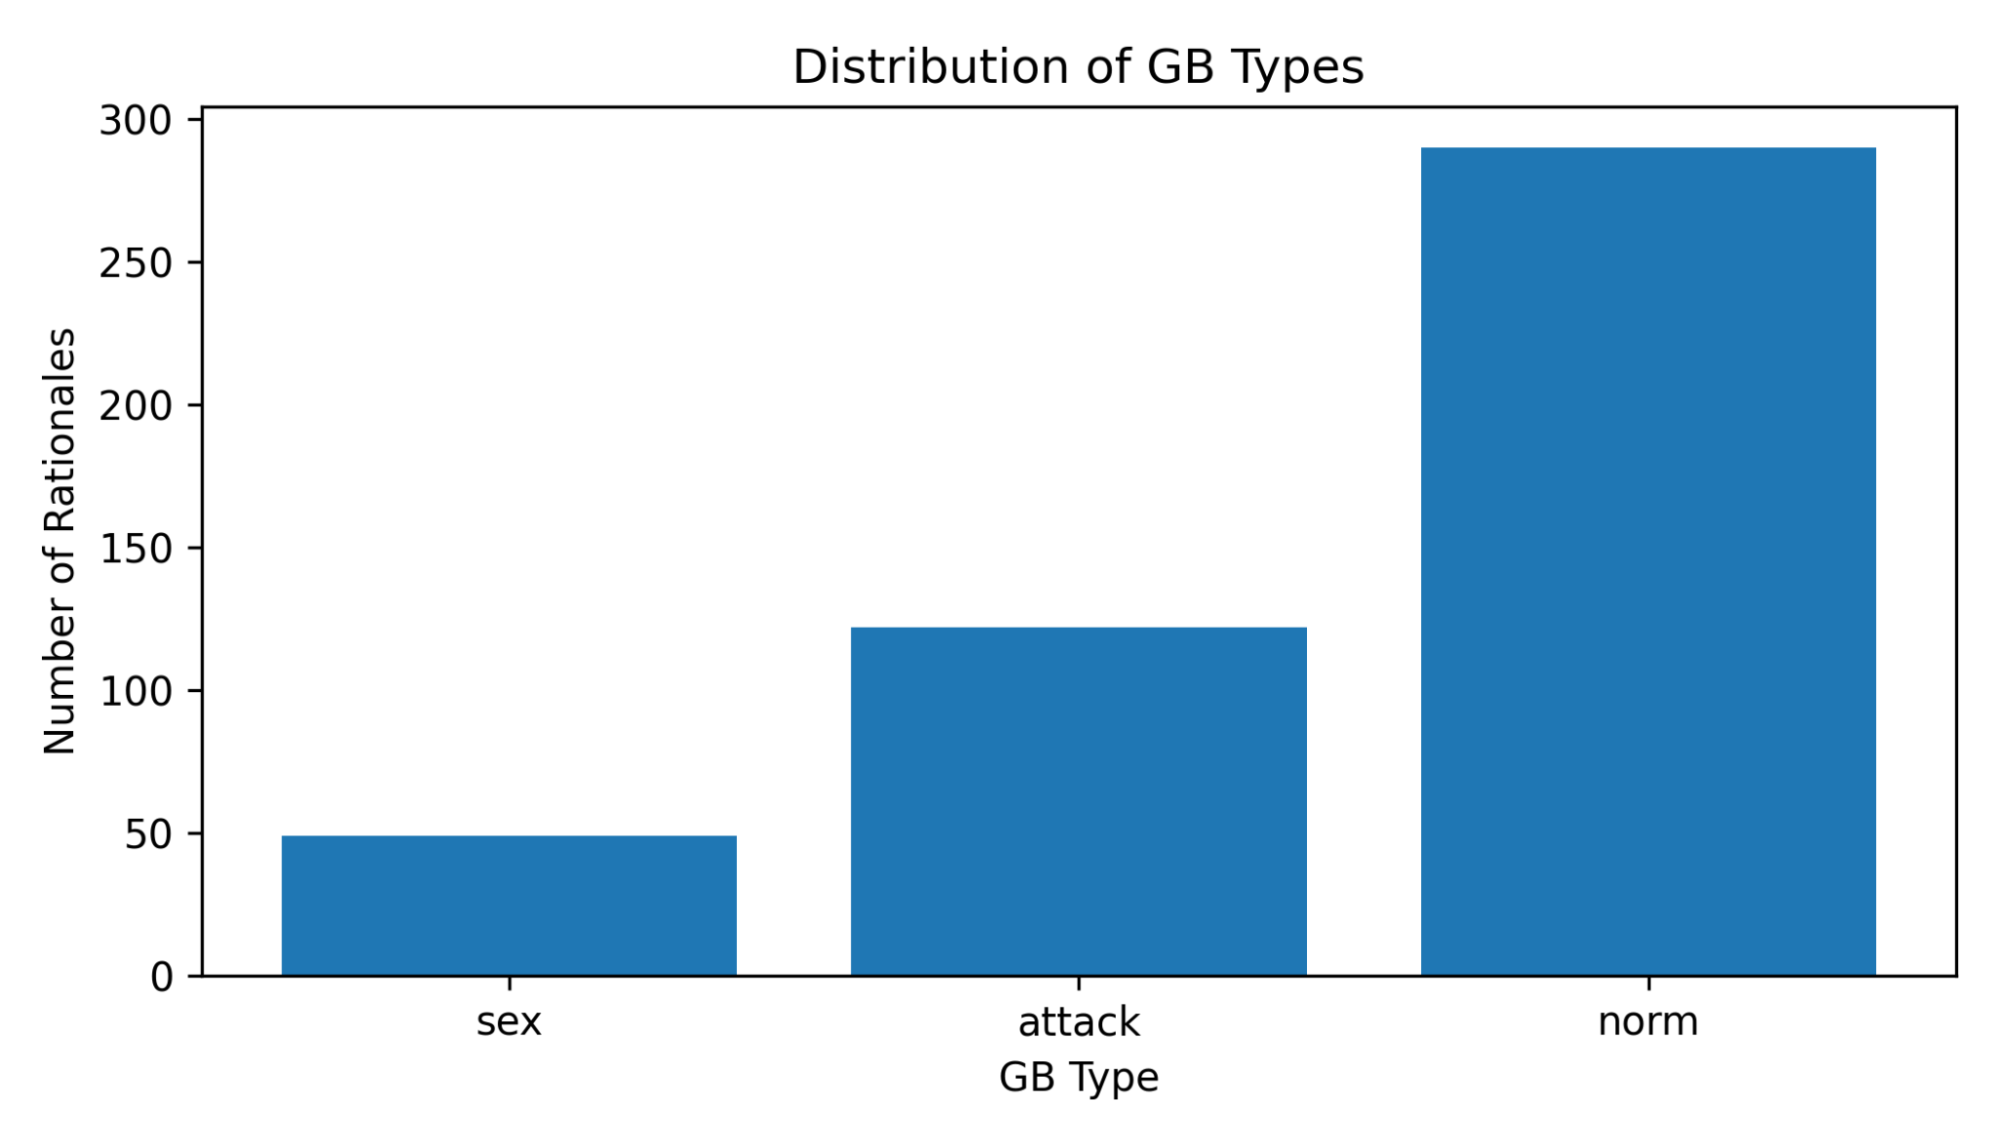
\includegraphics[width=0.8\linewidth]{assets/images/chapter4/image19.png}
\caption{Distribution of GB Types}
\label{fig:gb-type-distribution}
\end{figure}

For the GB subtype distribution in Figure~\ref{fig:gb-type-distribution}, GB-NORMATIVE is the most frequent subtype, with 290 rationales or 62.91\% of all GB rationales. This shows that gender bias in the annotated dataset most often appears in the form of stereotypes, gender-role expectations, norm enforcement, or identity policing. The second most common subtype is GB-ATTACK, with 122 rationales or 26.46\%, representing direct insults, derogatory language, or dehumanizing expressions toward gender or SOGI groups. The least frequent subtype is GB-SEX, with only 49 rationales or 10.63\%, showing that sexualized or body-based gendered insults are underrepresented in the current human-annotated dataset.

\begin{figure}[H]
\centering
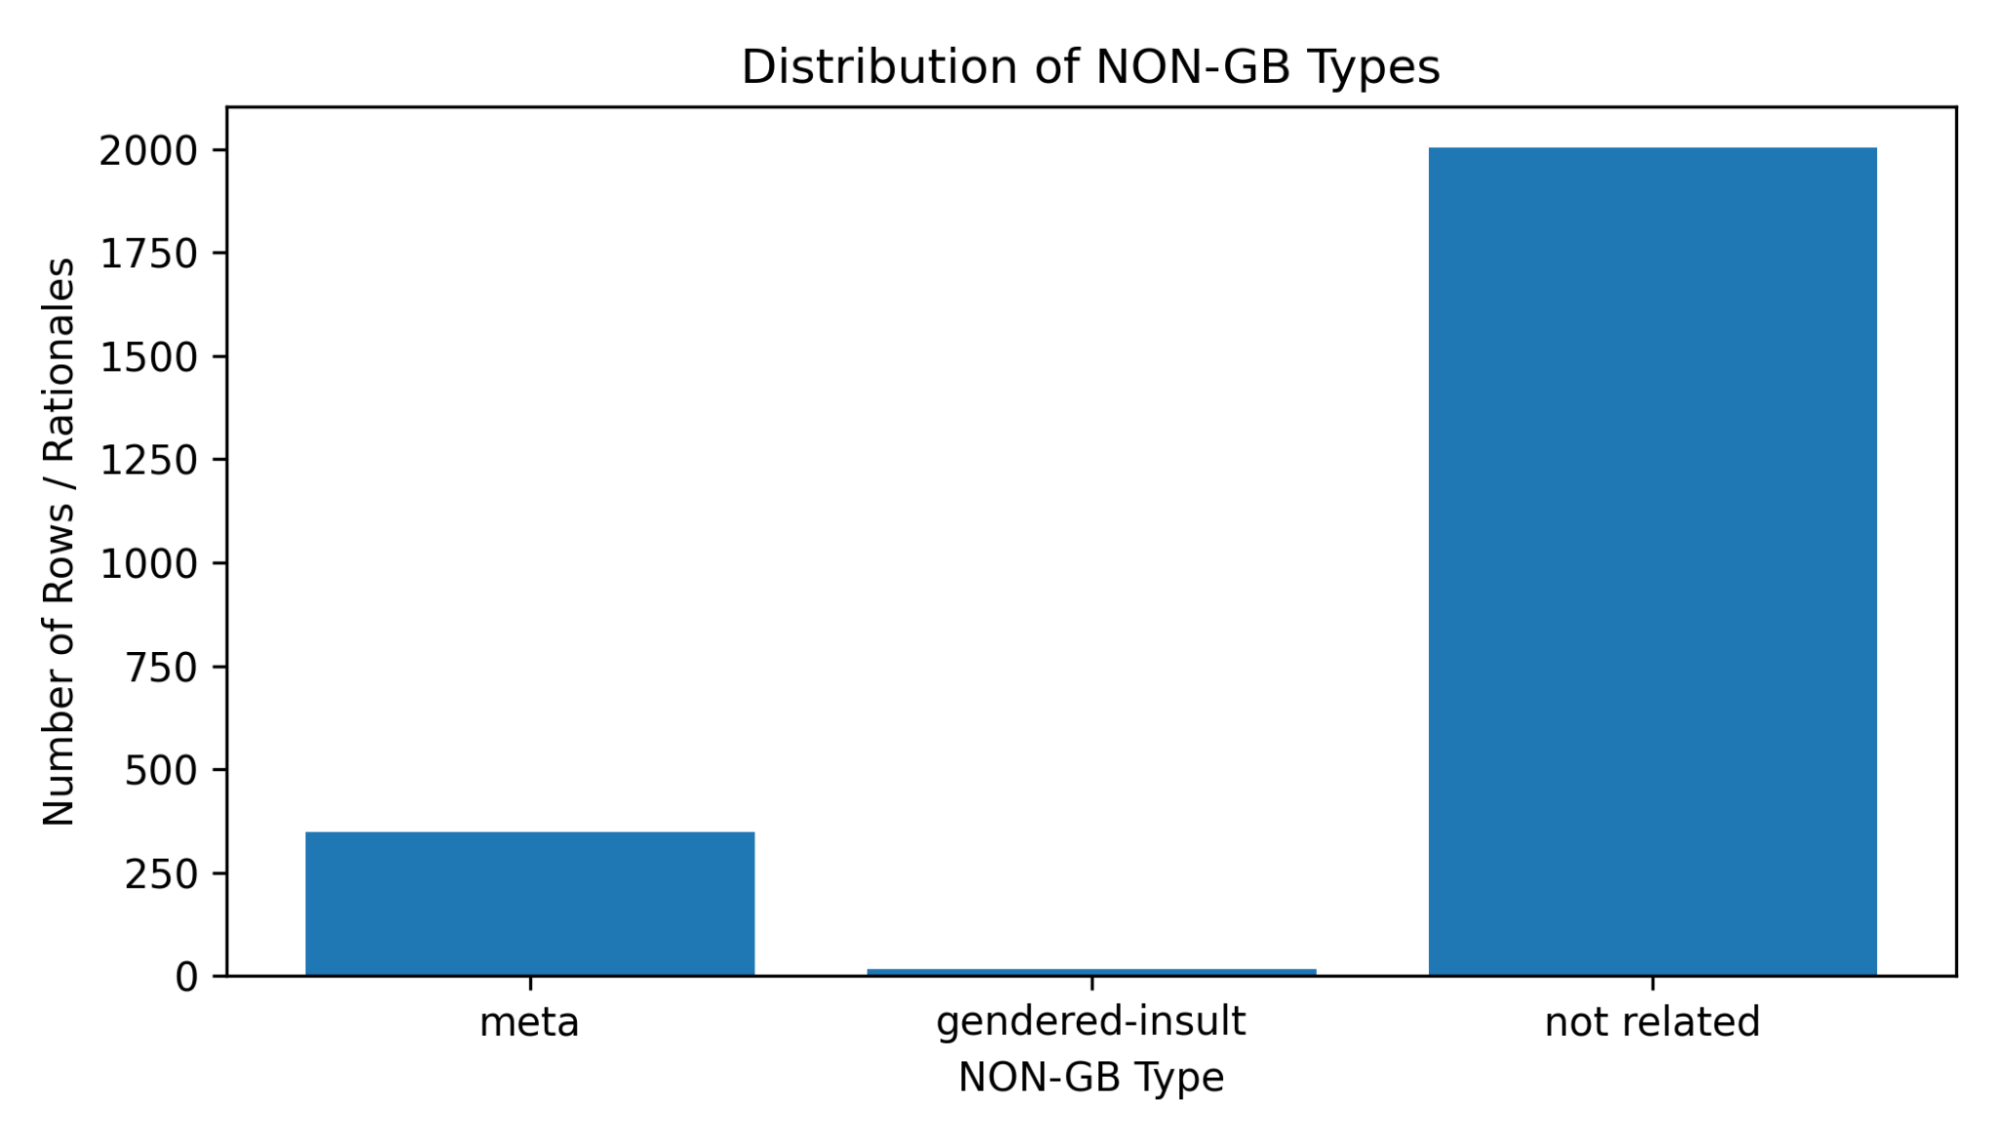
\includegraphics[width=0.8\linewidth]{assets/images/chapter4/image6.png}
\caption{Distribution of NON-GB Types}
\label{fig:non-gb-type-distribution}
\end{figure}

For NON-GB categories in Figure~\ref{fig:non-gb-type-distribution}, the largest group is not related, with 2,003 rows/rationales, accounting for 84.62\% of NON-GB cases. These are texts that do not contain gender-related bias or do not require rationale annotation. The meta category contains 348 cases or 14.70\%, representing social critique, counter-speech, or discussion of bias without expressing bias directly. The smallest NON-GB category is gendered-insult, with only 16 cases or 0.68\%, referring to cases where gender is mentioned while insulting a specific individual rather than a gender group.

Overall, the charts in Figure~\ref{fig:gender-bias-binary-label-distribution}, Figure~\ref{fig:gb-type-distribution}, and Figure~\ref{fig:non-gb-type-distribution} show two major imbalance problems. First, the dataset is highly imbalanced at the binary level, with NON-GB samples greatly outnumbering GB samples. Second, the GB subtypes are also imbalanced, with GB-NORMATIVE dominating the biased examples while GB-SEX has very few samples. This imbalance can affect model training because the model may learn to favor the majority classes and perform poorly on minority categories. For example, the model may become better at detecting common normative stereotypes but struggle to detect sexualized gender bias or rare gendered-insult cases.

To reduce this problem, synthetic data generation was introduced as a balancing strategy. By generating additional examples for underrepresented classes, especially minority GB subtypes such as GB-SEX and GB-ATTACK, the training dataset can provide the model with more diverse patterns of gender-biased language. This helps reduce class imbalance, improve model exposure to rare categories, and support more reliable classification across both binary and subtype labels.

\subsection{Impact of the Web Annotator Tool on Annotation Quality}

The preliminary analysis of LLM-generated prelabels revealed several limitations in automatic span selection, especially for fine-grained gender-bias triggers and rationales. The model sometimes selected incorrect span boundaries, merged unrelated tokens, or failed to clearly distinguish between trigger and rationale spans. Since the dataset requires token-level precision, these boundary errors could introduce labeling noise and affect bias subtype classification and decision-rule assignment.

In addition to the limitations of LLM-generated prelabels, early pilot annotation using raw text and static token lists was also difficult for annotators. Annotators had to manually compare guideline definitions, token sequences, bias categories, and decision rules, which increased the risk of inconsistent span selection and formatting errors. These issues showed that both automatic prelabeling and manual annotation without tool support were insufficient for producing reliable span-level annotations.

To address these problems, a dedicated web-based annotator tool was developed. The tool was designed based on the issues observed during the prelabeling experiment and pilot annotation process. Its purpose was to make span selection easier, reduce formatting errors, and improve consistency in applying the annotation guideline.

\subsubsection{Reduced Human Error Through Token-Level Highlighting}

The annotator tool helps reduce span boundary errors by displaying each sentence as a sequence of tokens. Annotators can directly highlight tokens to assign rationale and trigger spans, instead of manually typing token indices or editing raw JSON fields. This makes it easier to select minimal, guideline-compliant spans and reduces ambiguity during annotation.

\subsubsection{Integration With Decision Rules and Bias Taxonomy}

The tool also improves consistency by integrating the decision framework and bias taxonomy into the annotation interface. Annotators select the label type and decision rules directly inside the tool, reducing the need to recall all rule combinations manually. This helps ensure that each annotation includes the required information, such as the GB subtype or NON-GB label and the corresponding decision criteria.

\subsubsection{Streamlined Annotation Workflow}

The web annotator provides a more efficient annotation workflow. Annotators can upload CSV files containing sentence IDs and token sequences, annotate directly in the browser, and export the completed annotations in a standardized format. This reduces the amount of manual post-processing required and helps keep the annotation schema consistent across annotators.

\subsubsection{Improved Reproducibility and Quality Assurance}

The preview and export functions also support quality assurance. Before exporting, annotators can review the highlighted rationale and trigger spans to check whether the selected spans match the intended labels and decision rules. This allows annotation errors to be identified earlier and reduces the likelihood of downstream corrections during model training or evaluation.

\section{Model Training and Evaluation}

\subsection{Sentence-Level Model}

The sentence-level model was evaluated to measure its ability to classify Thai social-media text into gender-biased and non-gender-biased categories. The evaluation was conducted using the human-annotated dataset as a hard validation set, while the model itself was trained on the balanced synthetic corpus described in Section 3.6. This setup was used to test whether the model could generalize from synthetic training data to real annotated Thai social-media text.

\subsubsection{Training and Validation Data}

The synthetic training corpus contained 24,000 samples, with 4,000 samples per class across six sentence-level classes: GB-ATTACK, GB-NORMATIVE, GB-SEX, neutral, meta\_counter, and gendered\_insult. Since the corpus was generated using controlled prompts and passed quality filtering, no samples were removed before training.

For evaluation, the human-annotated dataset was used as the validation set. Binary evaluation was conducted on 717 rows with unambiguous GB or NON-GB ground-truth labels. For subtype evaluation, 392 GB rows were used, consisting of 243 GB-NORMATIVE, 109 GB-ATTACK, and 40 GB-SEX samples. The non-bias classes were not included in six-class subtype evaluation because many NON-GB rows did not map clearly to only one of the synthetic non-bias categories.

\subsubsection{Binary Classification Performance}

The binary evaluation groups GB-ATTACK, GB-NORMATIVE, and GB-SEX as Bias, while the non-bias labels are grouped as Not-Bias. The model achieved a macro-F1 score of 0.565 and an AUC-ROC of 0.561, indicating that it can distinguish biased from non-biased content above chance level, but still has considerable room for improvement. In this binary setting, the classifier was intentionally trained with visible gender-bias detection as the primary objective. Since the downstream use case is to surface potentially biased content for review, recall for the Bias class is prioritized over strict rejection of all non-biased text. The Bias class therefore achieved higher recall (0.760) than the Not-Bias class (0.385), showing that the model is more likely to capture biased sentences than to miss them. This behavior is appropriate for a screening-oriented bias detection system, where false negatives are more harmful than false positives. However, the tradeoff is that the model also flags some non-biased sentences as biased, which explains the lower Not-Bias recall and the need for later human review, threshold tuning, or stance-aware filtering.

\begin{table}[H]
\centering
\small
\caption{Binary Classification Performance of the Sentence-Level Model}
\begin{tabular}{@{}llll@{}}
\toprule
 & Precision & Recall & F1 \\
\midrule
Not-Bias & 0.571 & 0.385 & 0.460 \\
Bias & 0.598 & 0.760 & 0.670 \\
Macro avg & 0.585 & 0.572 & 0.565 \\
AUC-ROC & --- & --- & 0.561 \\
Accuracy & --- & --- & 0.590 \\
\bottomrule
\end{tabular}
\end{table}

\subsubsection{GB Subtype Classification Performance}

For subtype classification, the model was evaluated on the three GB categories: GB-ATTACK, GB-NORMATIVE, and GB-SEX. GB-NORMATIVE achieved the highest F1-score (0.606), likely because normative stereotypes appear more frequently in the synthetic training corpus and often follow more consistent lexical patterns. GB-ATTACK achieved a lower F1-score (0.396), while GB-SEX performed weakest (0.215). The low performance of GB-SEX is likely related to its small support in the human-annotated validation set, with only 40 instances, as well as the subtle and context-dependent nature of sexualized language in Thai social media.

The confusion patterns also show semantic overlap between categories. For example, GB-NORMATIVE was sometimes predicted as GB-ATTACK because normative statements can escalate into insulting or dehumanizing language. It was also sometimes predicted as \texttt{meta\_counter}, because gender-role statements may appear in discussion or critique contexts depending on the speaker's stance.

\begin{table}[H]
\centering
\small
\caption{GB Subtype Classification Performance of the Sentence-Level Model}
\begin{tabular}{@{}lllll@{}}
\toprule
Class & Precision & Recall & F1 & Support \\
\midrule
GB-ATTACK & 0.389 & 0.404 & 0.396 & 109 \\
GB-NORMATIVE & 0.763 & 0.502 & 0.606 & 243 \\
GB-SEX & 0.280 & 0.175 & 0.215 & 40 \\
Macro avg & 0.239 & 0.180 & 0.203 & 392 \\
\bottomrule
\end{tabular}
\end{table}

\subsubsection{Error Analysis}

To better understand the failure modes of the sentence-level classifier, a qualitative analysis was conducted on misclassified cases from the annotated validation set. The analysis focused on two main error directions: false positives, where NON-GB sentences were predicted as GB, and false negatives, where GB sentences were predicted as NON-GB.

A total of 1,002 false positives were observed. The largest group consists of 561 cases incorrectly predicted as GB-NORMATIVE. Many of these cases involve neutral or supportive mentions of gender or LGBTQ+ individuals, such as a speaker sharing a personal anecdote about a transgender friend or describing the demographic composition of a friend group without any evaluative framing. The model appears to over-fire on gender-related surface tokens such as ``กระเทย'', ``เกย์'', ``ผู้หญิง'', and ``ผู้ชาย'', regardless of the speaker's stance. As a result, it fails to distinguish neutral gender mentions from actual expressions of bias.

The second-largest false positive group contains 316 cases predicted as GB-ATTACK. These cases include counter-speech that uses slur terms in a supportive or defensive framing, general profanity unrelated to any gender target, and off-topic content such as anime discussion or celebrity gossip that shares surface-level features with attack language. For example, a sentence such as ``จะกระเทยหรือตุ๊ดมันก้อมีหัวใจไว้รักคนที่เรารัก'' contains gendered terms, but it expresses a supportive stance rather than an attack. This suggests that the model cannot reliably distinguish the direction of profanity, especially whether offensive language targets a gender group or appears in a non-biased context.

The remaining 125 false positives were incorrectly labeled as GB-SEX. These cases typically involve body-related mentions without gender-derogatory framing, such as personal preference statements or self-disclosure. In these cases, body-related tokens alone appear to trigger the sexualization prediction, even when the sentence does not devalue or shame a gender or SOGI group. Overall, the root cause across false positive cases is the model's reliance on lexical co-occurrence with gender terms, body-related tokens, or profanity. The model lacks sufficient pragmatic and discourse-level understanding to determine whether the speaker is expressing bias, quoting bias, criticizing bias, or speaking neutrally.

For false negatives, a total of 94 cases were observed, meaning the true label was GB but the model predicted NON-GB. Among these, 72 cases were incorrectly predicted as \texttt{meta\_counter}. This is the most revealing false negative pattern. Many of these cases are genuine gender-biased sentences, particularly GB-NORMATIVE instances, but they are written in a policy-discussion or concern-based register. Examples include statements expressing anxiety about LGBTQ+ rights ``affecting'' the majority, or identity-policing framed as a question of safety.

The model appears to use analytical or measured tone as a proxy for counter-speech. As a result, bias that is packaged as a reasoned argument is systematically missed. This reflects a failure to apply Criterion C of the annotation framework, which requires that the speaker must genuinely be criticizing bias rather than expressing bias under the guise of concern.

The remaining 20 false negatives were predicted as neutral. These cases involve very short texts, implicit cultural slurs such as ``ขุดทอง'', ``ถังขี้'', and ``หำรี'', or gender-role enforcement phrased without explicit negative evaluative language. The model appears to lack sufficient signal from the short token window and does not fully encode the idiom-level knowledge required to recognize these expressions as gendered bias.

\begin{table}[H]
\centering
\small
\caption{Error Analysis Summary for the Sentence-Level Model}
\begin{tabularx}{\textwidth}{@{}l r >{\raggedright\arraybackslash}X >{\raggedright\arraybackslash}X@{}}
\toprule
\textbf{Error type} & \textbf{Count} & \textbf{Primary pattern} & \textbf{Model weakness} \\
\midrule
FP $\rightarrow$ GB-NORMATIVE & 561 & Neutral / supportive gender mention & Fires on gender tokens regardless of speaker stance \\
FP $\rightarrow$ GB-ATTACK & 316 & Counter-speech, unrelated crude language & Cannot distinguish direction of profanity \\
FP $\rightarrow$ GB-SEX & 125 & Body mention without gender derogation & Body tokens treated as sexualisation signal \\
FN $\rightarrow$ meta\_counter & 72 & Bias framed as policy concern or analysis & Analytical tone conflated with counter-speech \\
FN $\rightarrow$ neutral & 20 & Short texts, implicit slurs, idioms & Insufficient token signal; no idiom knowledge \\
\bottomrule
\end{tabularx}
\end{table}

\subsubsection{Discussion}

The sentence-level model provides a useful baseline for Thai gender-bias classification, but the results show that synthetic-only training is not sufficient for robust real-world performance. Although the balanced synthetic corpus allowed the model to learn the overall label structure, the evaluation on human-annotated data reveals a clear domain gap between generated examples and real Thai social-media language.

The main limitation is stance sensitivity. The model often reacts to gender-related, body-related, or profane vocabulary without fully understanding whether the speaker is expressing bias, criticizing bias, quoting bias, or mentioning gender neutrally. This explains both the high number of false positives in NON-GB cases and the false negatives where biased statements are written in a more analytical or concern-based tone.

The subtype results also suggest that label complexity and class imbalance remain important challenges. GB-NORMATIVE is easier for the model to detect because it appears more frequently and often follows recognizable stereotype patterns, while GB-SEX remains difficult due to limited validation examples and the subtle, context-dependent nature of sexualized language in Thai social media.

Overall, these results should be interpreted as a baseline rather than a final model. Future improvement should focus on retraining with more human-annotated data, combining real and synthetic examples, increasing samples for minority classes such as GB-SEX, and adding stance-aware examples that include neutral gender mentions, counter-speech, implicit bias, and idiom-based expressions. In addition, future model designs should better encode speaker stance and discourse context, rather than relying mainly on token co-occurrence with gender-related or body-related terms.

\subsection{Span-Level Model}

The span-level detection component evaluates whether the model can identify biased text spans within input text. Unlike the sentence-level classifier, which predicts one label for the whole sentence, the span-level model outputs extracted spans grouped by GB subtype. The current span-level approach uses structured JSON output from a LoRA-fine-tuned generative model constrained to approximately 2 billion parameters. This approach was adopted after the initial BIO-tagging design was revised due to limited human-annotated span data, the difficulty of stance-sensitive classification, and the requirement for a model that could remain feasible for low-resource deployment.

At this stage, the span-level model should be interpreted as a preliminary extraction model rather than a fully deployable component. The model is evaluated on its ability to extract GB subtype spans, but it does not yet separately predict rationale spans and trigger spans in the same structure as the human annotation scheme.

\subsubsection{Evaluation Setup}

The span-level model was evaluated using the human-annotated dataset. The dataset contains 2,713 rows in total, of which 392 rows contain at least one GB label: GB-ATTACK, GB-NORMATIVE, or GB-SEX. Evaluation was conducted on these 392 GB rows because NON-GB rows do not contain ground-truth biased spans for measuring extraction quality.

Two complementary metrics were used: exact-match span F1 and character-level F1. Exact-match span F1 requires the predicted span string to match the ground-truth span exactly. Character-level F1 gives partial credit by measuring the overlap between characters in the predicted span and the human-annotated span. The difference between these two metrics helps diagnose the dominant error type. A large gap suggests that the model identifies the general biased region but extracts spans with inaccurate boundaries, while a small gap suggests that the model predicts spans in the wrong location.

\subsubsection{Quantitative Results}

The exact-match span results show that the current model performs poorly when strict span boundary matching is required. The overall macro-F1 is only 0.013, indicating that the model rarely produces spans that exactly match the human-annotated ground truth.

\begin{table}[H]
\centering
\small
\caption{Exact-Match Span F1 for the Span-Level Model}
\begin{tabular}{@{}lllllll@{}}
\toprule
Label & Precision & Recall & F1 & TP & FP & FN \\
\midrule
GB-NORMATIVE & 0.040 & 0.017 & 0.024 & 5 & 121 & 284 \\
GB-SEX & 0.013 & 0.020 & 0.016 & 1 & 74 & 48 \\
GB-ATTACK & 0.000 & 0.000 & 0.000 & 0 & 197 & 122 \\
Macro F1 & ~ & ~ & 0.013 & ~ & ~ & ~ \\
\bottomrule
\end{tabular}
\end{table}

The character-level evaluation shows higher performance than exact-match evaluation. The character-level macro-F1 is 0.296, suggesting that the model sometimes identifies relevant regions of biased text even when the extracted boundaries do not exactly match the annotated spans.

\begin{table}[H]
\centering
\small
\caption{Character-Level F1 for the Span-Level Model}
\begin{tabular}{@{}llll@{}}
\toprule
Label & Precision & Recall & F1 \\
\midrule
GB-NORMATIVE & 0.545 & 0.311 & 0.396 \\
GB-SEX & 0.177 & 0.312 & 0.226 \\
GB-ATTACK & 0.172 & 0.588 & 0.266 \\
Macro F1 & ~ & ~ & 0.296 \\
\bottomrule
\end{tabular}
\end{table}

The diagnostic gap between character-level F1 and exact-match F1 confirms that boundary errors are a major issue. GB-NORMATIVE has the largest gap of +0.372, followed by GB-ATTACK with +0.266 and GB-SEX with +0.210. This means that the model often extracts text near the correct biased region but does not match the human-selected span boundaries precisely.

\begin{table}[H]
\centering
\small
\caption{Diagnostic Gap Between Character-Level and Exact-Match Span F1}
\begin{tabular}{@{}lll@{}}
\toprule
Label & Gap & Interpretation \\
\midrule
GB-NORMATIVE & +0.372 & Boundary errors dominate \\
GB-SEX & +0.210 & Boundary errors dominate \\
GB-ATTACK & +0.266 & Boundary errors dominate \\
\bottomrule
\end{tabular}
\end{table}

The model also showed a high faithfulness rate, meaning that most predicted spans were copied directly from the input rather than hallucinated. Overall, 372 out of 398 predicted spans were faithful to the input, giving an overall faithfulness rate of 0.935.

\begin{table}[H]
\centering
\small
\caption{Faithfulness Rate of Predicted Spans}
\begin{tabular}{@{}llll@{}}
\toprule
Label & Faithful & Total & Rate \\
\midrule
GB-NORMATIVE & 116 & 126 & 0.921 \\
GB-SEX & 72 & 75 & 0.960 \\
GB-ATTACK & 184 & 197 & 0.934 \\
Overall & 372 & 398 & 0.935 \\
\bottomrule
\end{tabular}
\end{table}

\subsubsection{False Positive Analysis}

A total of 1,908 false positives were observed across the three GB labels: 1,121 for GB-ATTACK, 441 for GB-NORMATIVE, and 346 for GB-SEX. False positives were grouped into six error types using a heuristic diagnostic function that compares each predicted span against the ground-truth annotations and the source text.

\begin{table}[H]
\centering
\small
\caption{False Positive Breakdown for the Span-Level Model}
\begin{tabular}{@{}lllll@{}}
\toprule
Cause & GB-ATTACK & GB-NORMATIVE & GB-SEX & Total \\
\midrule
False alarm on NON-GB row & 924 & 320 & 272 & 1,516 \\
Present bias misclassified & 116 & 20 & 54 & 190 \\
Boundary shift (char overlap) & 49 & 65 & 16 & 130 \\
Over-extension (GT $\subset$ pred) & 21 & 19 & 2 & 42 \\
Spurious (no GT span for label) & 6 & 14 & 1 & 21 \\
Label confusion & 5 & --- & 1 & 6 \\
Over-extraction (pred $\subset$ GT) & --- & 3 & 1 & 4 \\
\bottomrule
\end{tabular}
\end{table}

The dominant error type is false alarm on NON-GB rows, accounting for 1,516 out of 1,908 false positives, or 79.5\% of all false positives. In these cases, the model extracts a span from a sentence that does not contain a ground-truth GB annotation. This suggests that the model overgeneralizes from surface gender-related tokens and extracts spans even when the surrounding context does not express gender bias. This pattern is similar to the sentence-level classifier, where gender terms such as ``ผู้หญิง'', ``กะเทย'', or ``ทอม'' often trigger bias predictions regardless of the speaker's intent.

The second most frequent error type is present bias misclassified, with 190 cases. In these cases, a genuine bias span exists in the row, but the model assigns it to the wrong GB subtype. This error is most common for GB-ATTACK, with 116 cases. It often occurs when GB-SEX content is predicted as GB-ATTACK or when directly attacking language and sexually derogatory language overlap. This reflects the semantic closeness between sexualized insults and direct attacks in Thai social-media text.

Boundary-related errors also explain the large gap between character-level F1 and exact-match F1. Boundary shift, over-extension, and over-extraction account for 176 cases in total. These errors show that the model often identifies the correct general region of biased text, but extracts spans that are too broad, too narrow, or slightly misaligned compared with the human annotation.

\subsubsection{Discussion}

The span-level model is not yet reliable enough for deployment. The exact-match macro-F1 of 0.013 shows that the model rarely matches human-annotated span boundaries exactly. However, the higher character-level macro-F1 of 0.296 and the faithfulness rate of 0.935 provide useful diagnostic insight. These results suggest that the model often copies text directly from the input and can sometimes locate relevant biased regions, but it struggles with precise boundary selection.

The main limitation is therefore not only span detection, but guideline-aligned span extraction. The model must learn to select spans according to the project's definition of minimal biased evidence, which is more specific than simply identifying a nearby gender-related phrase. This explains the large gap between character-level and exact-match performance.

The false positive analysis also shows that the model has not yet learned to condition extraction on speaker stance. It often reacts to gender-related terms without reliably distinguishing between bias, neutral mention, quotation, or counter-speech. Future improvement should focus on adding more human-annotated span examples, especially neutral gender mentions, counter-speech, implicit bias, and context-dependent expressions. Future work should also consider revising the output format to separately predict rationale and trigger spans once enough annotated data is available.

\chapter{Conclusion}

\section{Conclusion}

This project aimed to develop a Thai-language NLP system for detecting gender-biased language in social media text at both the sentence level and the span level. The work was conducted through five main stages: data collection, preprocessing and exploratory analysis, annotation guideline and tool development, model training, and evaluation.

The data collection phase produced a corpus of 52,055 unique Thai social media records from YouTube, Twitter/X, and TikTok. The dataset provides broad coverage of informal Thai language, slang, conversational expressions, and platform-specific writing styles relevant to gender-bias detection. Exploratory data analysis was conducted using both LDA-based topic modeling and BERTopic with Thai-compatible sentence embeddings. The BERTopic experiments showed that the corpus contains meaningful topic clusters related to gender stereotypes, sexualized language, identity policing, LGBTQ+ references, appearance-based insults, and harassment. Among the evaluated embedding models, Wangchan-SimCSE with unigram-bigram features produced the most coherent and culturally aligned topic structure. This supported the use of topic modeling as the main method for selecting higher-signal records for annotation.

The annotation stage produced a structured Gender Bias and SOGI Bias annotation guideline. The guideline defines a two-level label structure consisting of a binary GB/NON-GB distinction and three GB subtypes: GB-ATTACK, GB-NORMATIVE, and GB-SEX. It also introduces a decision framework based on Criteria A--D to help annotators distinguish true gender bias from neutral gender mentions, meta commentary, counter-speech, and single-person gendered insults. In addition, the guideline defines rationale and trigger span-selection rules to support interpretable span-level annotation. A browser-based web annotator tool was developed to reduce manual annotation errors, support token-level highlighting, enforce structured decision-rule selection, and export annotations in a consistent format.

Human annotation was conducted on 2,720 filtered records selected from gender- and SOGI-related topic groups. The resulting dataset contains 392 GB samples and 2,328 NON-GB samples, confirming that gender-biased content remains sparse even after topic-based filtering. The annotated data also showed clear class imbalance: GB-NORMATIVE was the most frequent subtype, while GB-SEX was the least frequent. This imbalance motivated the use of synthetic data generation to provide additional training examples for underrepresented categories.

For model development, the project implemented both sentence-level and span-level components. The sentence-level classifier used \texttt{microsoft/Multilingual-MiniLM-L12-H384} and was trained on a balanced synthetic corpus of 24,000 samples, with 4,000 samples per class. The human-annotated dataset was used as a hard validation set to evaluate generalization to real Thai social media text. In binary classification, the model achieved a macro-F1 score of 0.565 and an AUC-ROC of 0.561, indicating above-chance discrimination between biased and non-biased content. For subtype classification, GB-NORMATIVE achieved the strongest performance with an F1-score of 0.606, while GB-SEX performed weakest with an F1-score of 0.215, reflecting both limited support and the subtle nature of sexualized or body-based gender bias in Thai social media.

The span-level component was revised from the initial BIO-tagging design to a LoRA-based generative span extraction approach using Qwen3.5-2B-Base and the Unsloth framework. The model outputs structured JSON spans grouped by GB subtype rather than separate rationale and trigger predictions. Preliminary evaluation showed that the current span-level model is not yet reliable for deployment, with an exact-match macro-F1 of 0.013. However, the character-level macro-F1 of 0.296 and faithfulness rate of 0.935 suggest that the model can sometimes identify relevant biased regions and usually copies spans directly from the input rather than hallucinating text. The main challenge remains precise, guideline-aligned span boundary selection and reducing false alarms on NON-GB content.

Error analysis showed that the main weakness of the sentence-level model is stance sensitivity. The model often overpredicts GB when gender-related terms, body-related words, or profanity appear, even when the sentence is neutral, supportive, or counter-speech. It also struggles with bias framed as policy concern or analytical discussion, often misclassifying such cases as meta commentary. These findings show that synthetic-only training is useful for building an initial baseline, but it does not fully capture the ambiguity, slang, pragmatics, and context dependence of real Thai social media language.

Overall, this project produced several concrete outcomes: a large Thai social media corpus with platform metadata, a human-annotated gender-bias dataset with sentence-level labels and span annotations, a web-based annotation tool, a sentence-level classification baseline, and a preliminary span-level extraction model. Although the current system does not yet fully achieve separate rationale and trigger prediction, it establishes a foundation for interpretable Thai gender-bias detection and highlights key directions for future improvement, including expanding human annotation, incorporating conversational context, improving stance-aware modeling, and refining span-level extraction.

\section{Limitations and Challenges}

\subsection{Span-Level Detection Scope}

Although the project originally aimed to separately predict rationale spans and trigger spans, the current span-level model does not yet fully achieve this objective. The human-annotated dataset contains both rationale and trigger annotations, but the current generative span-level model outputs biased span strings grouped by GB subtype instead of producing separate rationale and trigger predictions. Therefore, the system can still highlight text regions related to gender bias, but it cannot yet distinguish between broader rationale context and minimal trigger cues in the same way as the human annotation scheme.

This limitation is mainly caused by the complexity of span-level supervision and the limited amount of human-annotated span data. Predicting rationale and trigger spans separately requires the model to learn fine-grained boundary decisions, subtype distinctions, and stance-sensitive interpretation. The preliminary span-level results suggest that the model often identifies relevant text regions but struggles with exact boundaries and overprediction, especially when gendered words appear in neutral or counter-speech contexts.

As a result, the project should be understood as having achieved sentence-level gender-bias detection and an initial form of interpretable span extraction, while full rationale-trigger extraction remains a future improvement. Future work should train the span-level model on more human-annotated examples and revise the output format so that rationale and trigger spans are predicted separately.

\subsection{Limited and Imbalanced Human-Annotated Training Data}

Another limitation of the project is that the real human-annotated dataset was not used as the main training set for the current sentence-level model. This is because the annotated dataset is still limited in size and highly imbalanced. After human annotation, only 392 rows were labeled as GB, while 2,328 rows were labeled as NON-GB. The GB subtype distribution is also uneven, with GB-NORMATIVE appearing much more frequently than GB-ATTACK and GB-SEX. Training directly on this dataset could cause the model to overfit to majority classes and perform poorly on underrepresented categories, especially GB-SEX.

To address this issue, the sentence-level model was trained using a synthetic dataset generated by Gemini 2.5 Flash. The synthetic dataset contains 24,000 samples, with 4,000 samples for each of the six sentence-level classes. This provided a larger and more balanced training set, allowing the model to learn the overall label structure before being tested on real data.

However, synthetic data cannot fully represent the complexity of real Thai social-media language. Real posts and comments contain slang, sarcasm, implicit bias, context-dependent meanings, neutral gender mentions, and counter-speech patterns that may not appear naturally in generated data. Therefore, the human-annotated dataset was used as a hard validation set to evaluate whether the model trained on synthetic data could generalize to real-world examples. Future work should expand the human-annotated dataset and combine real and synthetic samples during training to improve robustness and reduce the domain gap.

\subsection{Model Capacity and Overprediction}

The current models are relatively small compared with the complexity of the task and dataset structure. Gender-bias detection in Thai social media requires the model to understand informal spelling, slang, implicit references, speaker stance, counter-speech, and context-dependent meaning. A smaller model may rely too heavily on surface-level cues, such as gender terms, body-related words, or profanity, instead of understanding whether the sentence actually expresses gender bias.

This limitation can lead to overprediction, where neutral gender mentions, counter-speech, or general insults are incorrectly classified as GB. For example, a sentence that mentions ``ผู้หญิง'', ``ผู้ชาย'', ``เกย์'', or ``กะเทย'' may be predicted as biased even when the speaker is describing, supporting, or criticizing bias rather than expressing it. This issue appears in both sentence-level and span-level results, where the model tends to fire on gender-related tokens without fully capturing the surrounding context.

Future work should explore larger or more context-aware models, additional stance-sensitive training data, and training strategies that include neutral gender mentions and counter-speech examples. This may help the system distinguish true gender bias from surface-level gender references more reliably.

\subsection{Discontinued LLM Pre-Labeling Workflow}

An LLM pre-labeling workflow was initially explored to reduce manual annotation effort. The pipeline used Ollama with Qwen 2.5 7B to generate preliminary sentence-level labels, rationale spans, and trigger spans from tokenized Thai social media text. The model output was designed as structured JSON and was passed through a postprocessing step to clean invalid formatting, normalize span formats, and prepare the results for possible use in the web annotator.

Although the pipeline was technically functional, it was not reliable enough to be used in the final annotation process. The model sometimes produced invalid or non-strict JSON, inconsistent span formats, incomplete rationale or trigger spans, and unstable decisions for borderline cases such as meta commentary or counter-speech. More importantly, the model often failed to identify biased expressions or labeled clearly biased sentences as neutral. These issues would have introduced annotation noise if the pre-labels had been used directly.

As a result, the LLM pre-labeling workflow was discontinued as a core methodology. The final annotation process relied on human annotation through the web annotator tool instead. However, the experiment was still useful because it revealed the difficulty of automatic span-level gender-bias annotation and helped inform later design decisions, especially the need for stricter output formats, better validation, and clearer annotation guidelines.

\subsection{Thai Tokenization and Preprocessing Instability}

Thai tokenization remains a challenge because Thai text does not use spaces between words, and social media language often includes creative spelling, repeated characters, slang, emojis, mixed scripts, and irregular punctuation. Although PyThaiNLP's newmm tokenizer was used, token boundaries were not always stable for informal social media text. This affects span-level annotation because rationale and trigger spans depend on token indices.

Tokenization errors can increase annotator workload, create inconsistent span boundaries, and reduce the reliability of span-level evaluation. Preprocessing rules can also unintentionally alter expressive forms, such as repeated characters or slang, that may carry important pragmatic meaning. Future work should test neural Thai tokenizers such as DeepCut or compare multiple tokenization strategies, combined with careful normalization rules designed specifically for Thai social media.

\subsection{Synthetic-to-Real Domain Gap}

Although synthetic data helped address class imbalance, it introduced a domain gap between generated examples and real Thai social-media text. Synthetic examples are usually more controlled, complete, and guideline-like than real comments. In contrast, real social media posts contain slang, sarcasm, implicit bias, abbreviations, misspellings, neutral gender mentions, counter-speech, and context-dependent meanings.

This gap affected model performance. The sentence-level model learned from balanced synthetic patterns but struggled on real annotated data, especially when gender-related terms appeared in neutral or supportive contexts. This contributed to false positives on NON-GB cases and false negatives when biased statements were framed as policy discussion or ``reasonable concern.'' Future training should combine synthetic data with a larger human-annotated dataset, possibly using curriculum learning where the model is first trained on synthetic examples and then fine-tuned on real annotated data.

\subsection{Context Dependency in Social Media Text}

A further limitation is that many social media posts cannot be fully interpreted without surrounding context. This issue is especially important for TikTok comments, Twitter/X replies, and quoted posts, where a short comment may depend on the original video, tweet, or conversation thread. When viewed alone, a reply may appear neutral or unrelated, even though it carries gender-biased meaning in the original context.

Since annotation was mainly performed on extracted text records rather than full conversation threads, some context-dependent GB cases may have been labeled as NON-GB. This may partly explain the high proportion of NON-GB samples in the annotated dataset and the absence of TikTok from the GB distribution. Future work should collect and annotate more context, such as original posts, reply chains, quoted tweets, video captions, or surrounding comments, so that annotators and models can make more reliable decisions.

\subsection{Annotation Subjectivity and Guideline Complexity}

Gender-bias annotation is inherently interpretive, especially for borderline cases involving sarcasm, quoted bias, social critique, counter-speech, and single-person gendered insults. Even with a detailed guideline, annotators must judge whether the speaker is expressing bias or criticizing bias, whether a gender term refers to a group or an individual, and whether a phrase should be labeled as GB-ATTACK, GB-NORMATIVE, or GB-SEX.

The web annotator tool helped reduce formatting errors by supporting token-level highlighting, decision-rule selection, preview, and structured export. However, the tool cannot fully remove disagreement caused by subjective interpretation. Future work should include inter-annotator agreement measurement, adjudication sessions, and additional examples for confusing cases, especially Criterion C and Criterion D.

\section{Future Works}

\subsection{Expand and Balance the Human-Annotated Dataset}

The most important future improvement is to expand the human-annotated dataset. Priority should be given to minority and difficult categories, especially GB-SEX, GB-ATTACK, SOGI-related bias, gendered-insult cases, and counter-speech examples. A larger and more balanced dataset would improve both model training and evaluation, especially for subtype classification and span-level extraction.

\subsection{Incorporate Conversational Context}

Future annotation should include surrounding context, such as original tweets, quoted posts, TikTok video captions, YouTube video topics, and nearby comments in a thread. This would help annotators distinguish between neutral mentions, counter-speech, and true gender bias. It would also improve model training by giving the system access to the context needed for stance-sensitive classification.

\subsection{Combine Real and Synthetic Data for Training}

Once more human-annotated data is available, the sentence-level model should be retrained using a mixture of real and synthetic data. Synthetic examples can still be useful for balancing minority classes, but real examples are necessary for learning informal language, slang, sarcasm, and context-dependent expressions. A curriculum learning approach may also be useful, where the model is first trained on synthetic data and then fine-tuned on real annotated data.

\subsection{Improve Thai Tokenization for Social Media Text}

Future work should compare different Thai tokenizers, including neural tokenizers such as DeepCut, and evaluate their effect on span alignment. Additional preprocessing should focus on social media-specific normalization, including repeated characters, mixed Thai-English spelling, emojis, and slang. Better tokenization would improve annotation consistency and make span-level training more reliable.

\subsection{Develop Stance-Aware Modeling}

Future models should better encode speaker stance rather than relying mainly on gender-related token co-occurrence. Possible approaches include adding stance-detection auxiliary tasks, training on contrastive examples where the same gender term appears in biased and non-biased contexts, and incorporating discourse context from surrounding posts or comments. This would directly address the model's tendency to overpredict GB for neutral gender mentions and to miss bias framed as concern or policy discussion.

\subsection{Improve Span-Level Rationale and Trigger Prediction}

Future span-level models should be trained to output rationale spans and trigger spans separately. This would align the model more closely with the human annotation scheme. The output format may need to be revised from subtype-only JSON span extraction to a richer structure that includes rationale spans, trigger spans, GB subtype, and decision rules. The model should then be evaluated separately for rationale extraction, trigger extraction, subtype correctness, and boundary precision.

\subsection{Explore Larger or More Context-Aware Models}

Future experiments should test larger Thai-capable or multilingual models, such as WangchanBERTa, XLM-RoBERTa-large, or stronger instruction-tuned models. Larger models may better capture implicit bias, slang, sarcasm, and stance-sensitive phrasing. However, computational cost and deployment constraints should still be considered, especially if the final system is intended for lightweight or browser-based use.

\subsection{Optimize for Browser-Based Deployment}

The long-term deployment objective for the span-level component is to develop a browser-based interface or extension capable of highlighting gender-biased spans directly on social media pages. This would allow users to inspect potentially biased language in real time and improve the practical usability of the system.

Achieving this objective requires further optimization of the span-level model for low-latency inference. The current generative span extractor is approximately 2 billion parameters, which still requires considerable computational resources and is not yet suitable for lightweight on-device or browser-based deployment. Potential improvement strategies include INT4 or INT8 quantization, speculative decoding, model distillation, or replacing the generative span extractor with a smaller discriminative span-classification model once sufficient annotated span-level data becomes available.

\subsection{Maintain and Update the Dataset Over Time}

Gender-biased language changes quickly on social media. New slang, coded terms, memes, and platform-specific expressions may appear over time. Future work should include periodic re-scraping, annotation updates, and guideline revision so that the dataset and model remain relevant to current Thai online discourse.

%%%%%%%%%%%%%%%%%%%%%%%%%%%%%%%%%%%%%%%%%%%%%%%%%%%%%%%%%%%%%%%
%%%%%%%%%%%%%%%%%%%% Bibliography %%%%%%%%%%%%%%%%%%%%%%%%%%%%%
%%%%%%%%%%%%%%%%%%%%%%%%%%%%%%%%%%%%%%%%%%%%%%%%%%%%%%%%%%%%%%%

% Sept, 2021 by Thanin
% improve url breaks to prevent unnecessary big white spaces in some cases
\makeatletter
\g@addto@macro{\UrlBreaks}{\UrlOrds}
\makeatother
%

\begin{thebibliography}{53}

\bibitem{ref1}\hypertarget{bib:ref1}{} iLaw, ``\#สมรสเท่าเทียม : เปิดกฎหมายแพ่งแก้ไขใหม่ บุคคล-บุคคล สมรสได้
ไม่จำกัดแค่ชาย-หญิง,'' iLaw, Sep.~24, 2024. {[}Online{]}. Available:
\href{https://www.ilaw.or.th/articles/43563?utm_source=chatgpt.com}{https://www.ilaw.or.th/articles/43563}

\bibitem{ref2}\hypertarget{bib:ref2}{} R. Jennings, ``Taiwan's high court paves the way for same-sex
marriage, a first in Asia,'' Los Angeles Times, May 24, 2017.
{[}Online{]}. Available:
\href{https://www.latimes.com/world/la-fg-taiwan-same-sex-marriage-20170524-story.html?utm_source=chatgpt.com}{https://www.latimes.com/world/la-fg-taiwan-same-sex-marriage-20170524-story.html}

\bibitem{ref3}\hypertarget{bib:ref3}{} Amnesty International, ``Thailand: State-backed digital violence
silences women and LGBTI activists,'' \emph{Amnesty International Report
ASA39/7955/2024}, 2024. {[}Online{]}. Available:
\href{https://www.amnesty.org/en/documents/asa39/7955/2024/en?utm_source=chatgpt.com}{https://www.amnesty.org/en/documents/asa39/7955/2024/en}

\bibitem{ref4}\hypertarget{bib:ref4}{} TheGlobalEconomy.com, ``Thailand: Female labor force
participation,'' \emph{TheGlobalEconomy.com}, 2024. {[}Online{]}.
Available:
\href{https://www.theglobaleconomy.com/Thailand/Female_labor_force_participation?utm_source=chatgpt.com}{https://www.theglobaleconomy.com/Thailand/Female\_labor\_force\_participation}

\bibitem{ref5}\hypertarget{bib:ref5}{} TheGlobalEconomy.com, ``Thailand: Male labor force
participation,'' \emph{TheGlobalEconomy.com}, 2024. {[}Online{]}.
Available:
\href{https://www.theglobaleconomy.com/Thailand/Male_labor_force_participation?utm_source=chatgpt.com}{https://www.theglobaleconomy.com/Thailand/Male\_labor\_force\_participation}

\bibitem{ref6}\hypertarget{bib:ref6}{} K. Chanvised, ``Young Thai Women's Negotiation of Gender
Identity through Social Media,'' Ph.D.~dissertation, University College
London (UCL), 2022. {[}Online{]}. Available:
\url{https://discovery.ucl.ac.uk/id/eprint/10148350/1/Thesis_Kamolmas_Chanvised.pdf}

\bibitem{ref7}\hypertarget{bib:ref7}{} S. Yimwilai, ``Misogynistic Language in Thai and English: A
Comparative Study of Linguistic Features and Cultural Implications,''
\emph{Vacana Journal of Language and Communication}, vol.~11, no. 1,
pp.~21--40, 2022. {[}Online{]}. Available:
\url{http://rs.mfu.ac.th/ojs/index.php/vacana/article/view/351/251}

\bibitem{ref8}\hypertarget{bib:ref8}{} S. Trisin, ``Social Media, Body Norms, and Gendered Bodies,''
\emph{Humanities, Arts and Social Sciences Studies (HASS Journal)},
vol.~20, no. 1, pp.~199--222, 2020. {[}Online{]}. Available:
\url{https://so02.tci-thaijo.org/index.php/hasss/article/view/245364}

\bibitem{ref9}\hypertarget{bib:ref9}{} European Institute for Gender Equality (EIGE), ``Gender bias,''
\emph{EIGE Gender Equality Glossary \& Thesaurus}, 2016. {[}Online{]}.
Available:
\url{https://eige.europa.eu/publications-resources/thesaurus/terms/1320}

\bibitem{ref10}\hypertarget{bib:ref10}{} European Institute for Gender Equality (EIGE), ``Gender
stereotypes,'' \emph{EIGE Gender Equality Glossary \& Thesaurus}, 2016.
{[}Online{]}. Available:
\url{https://eige.europa.eu/publications-resources/thesaurus/terms/1223?language_content_entity=en}

\bibitem{ref11}\hypertarget{bib:ref11}{} European Institute for Gender Equality (EIGE), ``Sexism,''
\emph{EIGE Gender Equality Glossary \& Thesaurus}, 2016. {[}Online{]}.
Available:
\url{https://eige.europa.eu/publications-resources/thesaurus/terms/1325}

\bibitem{ref12}\hypertarget{bib:ref12}{} Cambridge Dictionary, ``Derogatory,'' \emph{Cambridge English
Dictionary}, 2024. {[}Online{]}. Available:
\url{https://dictionary.cambridge.org/dictionary/english/derogatory}

\bibitem{ref13}\hypertarget{bib:ref13}{} Cambridge Dictionary, ``Objectification,'' \emph{Cambridge
English Dictionary}, 2024. {[}Online{]}. Available:
\url{https://dictionary.cambridge.org/dictionary/english/objectification}

\bibitem{ref14}\hypertarget{bib:ref14}{} Cambridge Dictionary, ``Sexualization,'' \emph{Cambridge
English Dictionary}, 2024. {[}Online{]}. Available:
\url{https://dictionary.cambridge.org/dictionary/english/sexualization}

\bibitem{ref15}\hypertarget{bib:ref15}{} GeeksforGeeks, ``Getting started with Transformers,''
\emph{GeeksforGeeks Machine Learning Tutorials}, 2022. {[}Online{]}.
Available:
\url{https://www.geeksforgeeks.org/machine-learning/getting-started-with-transformers/}

\bibitem{ref16}\hypertarget{bib:ref16}{} GeeksforGeeks, ``Multi-head Attention Mechanism in NLP,''
\emph{GeeksforGeeks NLP Tutorials}, 2022. {[}Online{]}. Available:
\url{https://www.geeksforgeeks.org/nlp/multi-head-attention-mechanism/}

\bibitem{ref17}\hypertarget{bib:ref17}{} Indeed Editorial Team, ``Classifiers in Machine Learning: A
Guide,'' \emph{Indeed Career Guide}, 2023. {[}Online{]}. Available:
\url{https://www.indeed.com/career-advice/career-development/classifiers-in-machine-learning}

\bibitem{ref18}\hypertarget{bib:ref18}{} Analytics Steps, ``Types of Classifiers in Machine Learning,''
\emph{Analytics Steps Blog}, 2022. {[}Online{]}. Available:
\url{https://www.analyticssteps.com/blogs/types-classifiers-machine-learning}

\bibitem{ref19}\hypertarget{bib:ref19}{} D. Röder, A. Both, and A. Hinneburg, ``Exploring the space of
topic coherence measures,'' in Proc. WSDM, 2015. {[}Online{]}.
Available:
\url{https://svn.aksw.org/papers/2015/WSDM_Topic_Evaluation/public.pd}

\bibitem{ref20}\hypertarget{bib:ref20}{} GeeksforGeeks, ``Evaluation Metrics in Machine Learning,''
GeeksforGeeks Machine Learning Tutorials, Mar.~30, 2026. {[}Online{]}.
Available:
\url{https://www.geeksforgeeks.org/machine-learning/metrics-for-machine-learning-model/}

\bibitem{ref21}\hypertarget{bib:ref21}{} M. Brenndoerfer, ``BIO Tagging: Encoding Entity Boundaries for
Sequence Labeling,'' Michael Brenndoerfer, Apr.~12, 2025, updated
Jan.~3, 2026. {[}Online{]}. Available:
\href{https://mbrenndoerfer.com/writing/bio-tagging-sequence-labeling-ner/?utm_source=chatgpt.com}{https://mbrenndoerfer.com/writing/bio-tagging-sequence-labeling-ner/}

\bibitem{ref22}\hypertarget{bib:ref22}{} H. Correa, ``Effective Prompt Engineering: Mastering XML Tags
for Clarity, Precision, and Security in LLMs,'' Medium, Jun.~18, 2025.
{[}Online{]}. Available:
\href{https://medium.com/@TechforHumans/effective-prompt-engineering-mastering-xml-tags-for-clarity-precision-and-security-in-llms-992cae203fdc}{https://medium.com/@TechforHumans/effective-prompt-engineering-mastering-xml-tags-for-clarity-precision-and-security-in-llms-992cae203fdc}

\bibitem{ref23}\hypertarget{bib:ref23}{} OpenAI, ``Structured model outputs,'' OpenAI API Documentation.
{[}Online{]}. Available:
\href{https://developers.openai.com/api/docs/guides/structured-outputs?utm_source=chatgpt.com}{https://developers.openai.com/api/docs/guides/structured-outputs}

\bibitem{ref24}\hypertarget{bib:ref24}{} E. Karatas, ``Structured Output Generation in LLMs: JSON Schema
and Grammar-Based Decoding,'' Medium, Feb.~15, 2025. {[}Online{]}.
Available:
\href{https://medium.com/@emrekaratas-ai/structured-output-generation-in-llms-json-schema-and-grammar-based-decoding-6a5c58b698a6}{https://medium.com/@emrekaratas-ai/structured-output-generation-in-llms-json-schema-and-grammar-based-decoding-6a5c58b698a6}

\bibitem{ref25}\hypertarget{bib:ref25}{} J. Lu, ``LoRA Explained: Parameter-efficient fine-tuning,''
Medium, Jun.~2, 2024. {[}Online{]}. Available:
\href{https://lush93md.medium.com/lora-parameter-efficient-fine-tuning-8b12face1894?utm_source=chatgpt.com}{https://lush93md.medium.com/lora-parameter-efficient-fine-tuning-8b12face1894}

\bibitem{ref26}\hypertarget{bib:ref26}{} IBM, ``Low-rank adaptation (LoRA) fine tuning,'' IBM watsonx
Documentation. {[}Online{]}. Available:
\href{https://www.ibm.com/docs/en/watsonx/w-and-w/2.1.0?topic=tuning-lora-fine&utm_source=chatgpt.com}{https://www.ibm.com/docs/en/watsonx/w-and-w/2.1.0?topic=tuning-lora-fine}

\bibitem{ref27}\hypertarget{bib:ref27}{} A. Sooriyarachchi, ``Efficient Fine-Tuning with LoRA: A Guide
to Optimal Parameter Selection for Large Language Models,'' Databricks
Blog, Mar.~26, 2024. {[}Online{]}. Available:
\url{https://www.databricks.com/blog/efficient-fine-tuning-lora-guide-llms}

\bibitem{ref28}\hypertarget{bib:ref28}{} R. Kumar, ``What is MMLU? LLM Benchmark Explained and Why It
Matters,'' DataCamp, Jun.~11, 2025. {[}Online{]}. Available:
\href{https://www.datacamp.com/blog/what-is-mmlu?utm_source=chatgpt.com}{https://www.datacamp.com/blog/what-is-mmlu}

\bibitem{ref29}\hypertarget{bib:ref29}{} Confident AI, ``MMLU,'' DeepEval Documentation. {[}Online{]}.
Available:
\href{https://deepeval.com/docs/benchmarks-mmlu?utm_source=chatgpt.com}{https://deepeval.com/docs/benchmarks-mmlu}

\bibitem{ref30}\hypertarget{bib:ref30}{} K. Pasupa, W. Karnbanjob, and M. Aksornsiri, ``Hate Speech
Detection in Thai Social Media with Ordinal-Imbalanced Text
Classification,'' \emph{Proc. 2022 IEEE International Conference on Big
Data (Big Data)}, Osaka, Japan, pp.~5661--5667, 2022. {[}Online{]}.
Available: \url{https://ieeexplore.ieee.org/document/9836312}

\bibitem{ref31}\hypertarget{bib:ref31}{} L. Havens, M. Terras, B. Bach, and B. Alex, ``Situated Data,
Situated Systems: A Methodology to Engage with Power Relations in
Natural Language Processing Research,'' \emph{Proc. 1st Workshop on
Gender Bias in Natural Language Processing (GeBNLP)}, ACL, pp.~107--114,
2020. {[}Online{]}. Available:
\url{https://aclanthology.org/2020.gebnlp-1.10.pdf}

\bibitem{ref32}\hypertarget{bib:ref32}{} B. Mathew, P. Saha, S. M. Yimam, C. Biemann, P. Goyal, and A.
Mukherjee, ``HateXplain: A Benchmark Dataset for Explainable Hate Speech
Detection,'' \emph{arXiv Preprint}, arXiv:2012.10289, 2020.
{[}Online{]}. Available: \url{https://arxiv.org/pdf/2012.10289}

\bibitem{ref33}\hypertarget{bib:ref33}{} J. Zhao, T. Wang, M. Yatskar, V. Ordonez, and K. Chang,
``Gender Bias in Coreference Resolution: Evaluation and Debiasing
Methods,'' \emph{Proc. NAACL-HLT}, pp.~15--20, 2018. {[}Online{]}.
Available: \url{https://aclanthology.org/N18-2003.pdf}

\bibitem{ref34}\hypertarget{bib:ref34}{} A. Sahitaj, P. Sahitaj, V. Solopova1, J. Li, S.Möller, and V.
Schmitt, ``Hybrid Annotation for Propaganda Detection: Integrating LLM
Pre-Annotations with Human Intelligence,'' \emph{arXiv Preprint},
arXiv:2507.18343, 2025. {[}Online{]}. Available:
\url{https://arxiv.org/pdf/2507.18343}

\bibitem{ref35}\hypertarget{bib:ref35}{} P. Chormai, P. Prasertsom, J. Cheevaprawatdomrong, and A. T.
Rutherford, ``Syllable-Based Neural Thai Word Segmentation,''
\emph{Proc. COLING 2020}, pp.~4480--4491, 2020. {[}Online{]}. Available:
\url{https://aclanthology.org/2020.coling-main.407.pdf}

\bibitem{ref36}\hypertarget{bib:ref36}{} A. Vaswani, N. Shazeer, N. Parmar, J. Uszkoreit, L. Jones, A.
N. Gomez, Ł. Kaiser, and I. Polosukhin, ``Attention Is All You Need,''
\emph{Advances in Neural Information Processing Systems (NeurIPS)},
pp.~5998--6008, 2017. {[}Online{]}. Available:
\url{https://arxiv.org/pdf/1706.03762}

\bibitem{ref37}\hypertarget{bib:ref37}{} C. McDonald and D. Chiang, ``Syntax-Based Attention Masking for
Neural Machine Translation,'' \emph{Proc. NAACL Student Research
Workshop (SRW)}, pp.~1--8, 2021. {[}Online{]}. Available:
\url{https://aclanthology.org/2021.naacl-srw.7.pdf}

\bibitem{ref38}\hypertarget{bib:ref38}{} P. Zhang, B. Chen, N. Ge, and K. Fan, ``Long-Short Term Masking
Transformer: A Simple but Effective Baseline for Document-level Neural
Machine Translation,'' \emph{Proc. EMNLP 2020}, pp.~5463--5475, 2020.
{[}Online{]}. Available:
\url{https://aclanthology.org/2020.emnlp-main.81.pdf}

\bibitem{ref39}\hypertarget{bib:ref39}{} C. Saetia, E. Chuangsuwanich, T. Chalothorn, and P. Vateekul,
``Semi-Supervised Thai Sentence Segmentation Using Local and Distant
Word Representations,'' \emph{arXiv Preprint}, arXiv:1908.01294, 2019.
{[}Online{]}. Available: \url{https://arxiv.org/pdf/1908.01294}

\bibitem{ref40}\hypertarget{bib:ref40}{} Y. Lei, R. Huang, L. Wang, and N. Beauchamp, ``Sentence-level
Media Bias Analysis Informed by Discourse Structures,'' \emph{Proc.
EMNLP 2022}, pp.~9936--9952, 2022. {[}Online{]}. Available:
\url{https://aclanthology.org/2022.emnlp-main.682.pdf}

\bibitem{ref41}\hypertarget{bib:ref41}{} P. G. Hoang, C. D. Luu, K. Q. Tran, K. V. Nguyen, and N. L.-T.
Nguyen, ``ViHOS: Hate Speech Spans Detection for Vietnamese,''
\emph{arXiv Preprint}, arXiv:2301.10186, 2023. {[}Online{]}. Available:
\url{https://arxiv.org/pdf/2301.10186}

\bibitem{ref42}\hypertarget{bib:ref42}{} C. F. Moreno-García, E. Elyan, and C. Jayne, ``Heuristics-Based
Detection to Improve Text/Graphics Segmentation in Complex Engineering
Drawings,'' \emph{CORE Open Research Archive}, 2019. {[}Online{]}.
Available: \url{https://core.ac.uk/download/pdf/287597067.pdf}

\bibitem{ref43}\hypertarget{bib:ref43}{} L. Fan, M. White, E. Sharma, R. Su, P. K. Choubey, R. Huang,
and L. Wang, ``In Plain Sight: Media Bias Through the Lens of Factual
Reporting,'' \emph{Proc. EMNLP 2019}, pp.~3572--3578, 2019.
{[}Online{]}. Available: \url{https://aclanthology.org/D19-1664.pdf}

\bibitem{ref44}\hypertarget{bib:ref44}{} N. Panitsrisit, ``Thai Sentence Segmentation Using Large
Language Models,'' M.Sc. thesis, Chulalongkorn University, 2023.
{[}Online{]}. Available:
\url{https://digital.car.chula.ac.th/chulaetd/8113/}

\bibitem{ref45}\hypertarget{bib:ref45}{} P. Chiril, V. Moriceau, F. Benamara, A. Mari, G. Origgi, and M.
Coulomb-Gully, ``An Annotated Corpus for Sexism Detection in French
Tweets,'' \emph{Proc. LREC 2020}, pp.~7587--7595, 2020. {[}Online{]}.
Available: \url{https://aclanthology.org/2020.lrec-1.175/}

\bibitem{ref46}\hypertarget{bib:ref46}{} H. Kataria, A. Gupta, and V. Mishra, ``BennettNLP at
SemEval-2021 Task 5: Toxic Spans Detection using Stacked Embedding
Powered Toxic Entity Recognizer,'' in Proceedings of the 15th
International Workshop on Semantic Evaluation (SemEval-2021),
pp.~941--947, 2021. {[}Online{]}. Available:
\url{https://aclanthology.org/2021.semeval-1.128.pdf}

\bibitem{ref47}\hypertarget{bib:ref47}{} L. Bansal and N. Mishra, ``CREST: Universal Safety Guardrails
Through Cluster-Guided Cross-Lingual Transfer,'' arXiv preprint,
arXiv:2512.02711, 2025. {[}Online{]}. Available:
\url{https://arxiv.org/pdf/2512.02711v1}

\bibitem{ref48}\hypertarget{bib:ref48}{} F. Zhang, ``one-for-all-toxicity-v3,'' Hugging Face Model
Repository, 2023. {[}Online{]}. Available:
\url{https://huggingface.co/FredZhang7/one-for-all-toxicity-v3}

\bibitem{ref49}\hypertarget{bib:ref49}{} Unsloth AI, ``Unsloth: Run and train open models locally,''
GitHub Repository. {[}Online{]}. Available:
\url{https://github.com/unslothai/unsloth}

\bibitem{ref50}\hypertarget{bib:ref50}{} T. (Author from Thammasat University Thesis),
``การตรวจจับอคติทางเพศในสื่อสังคมออนไลน์ไทยด้วยวิธีการประมวลผลภาษาธรรมชาติ,''
Master's Thesis, Thammasat University, 2024. {[}Online{]}. Available:\\
\url{https://ethesisarchive.library.tu.ac.th/thesis/2024/TU_2024_6206034099_19373_29755.pdf}

\bibitem{ref51}\hypertarget{bib:ref51}{} SOS Children's Villages Thailand, ``Unfunny Jokes? การล้อเลียนกลุ่ม
LGBTQ+ ไม่ใช่เรื่องตลก,'' 2024. {[}Online{]}. Available:\\
\href{https://www.sosthailand.org/blogs/2024/unfunny-jokes-lgbtq?srsltid=AfmBOorN42mR3m3S6h5_9Hu0v-9FI5MBZxO--SA9JJTwhBH4ZZUnzPgz}{https://www.sosthailand.org/blogs/2024/unfunny-jokes-lgbtq?srsltid=AfmBOorN42mR3m3S6h5\_9Hu0v-9FI5MBZxO--SA9JJTwhBH4ZZUnzPgz}

\bibitem{ref52}\hypertarget{bib:ref52}{} The MATTER, ``From Black Bean to Santorum:
สำรวจประวัติศาสตร์คำด่าที่ทำร้ายเพศสภาพและเพศวิถี,'' 2024. {[}Online{]}.
Available:\\
\url{https://thematter.co/thinkers/from-black-bean-to-santorum/13160}

\bibitem{ref53}\hypertarget{bib:ref53}{} R. Korakot and W. Ruktanonchai, ``DeepCut: Thai Word Tokenizer
Using Neural Networks,'' GitHub Repository, 2016. {[}Online{]}.
Available: \url{https://github.com/rkcosmos/deepcut}

\end{thebibliography}

%%%%%%%%%%%%%%%%%%%%%%%%%%%%%%%%%%%%%%%%%%%%%%%%%%%%%%%%%%%%%%%
%%%%%%%%%%%%%%%%%%%%%%%% Appendix %%%%%%%%%%%%%%%%%%%%%%%%%%%%%
%%%%%%%%%%%%%%%%%%%%%%%%%%%%%%%%%%%%%%%%%%%%%%%%%%%%%%%%%%%%%%%
% There are multiple appendices.
\def\appendixnames{Appendices}
% No automatic running numbers for appendix headings.
\setcounter{secnumdepth}{-1}
% Keep ToC appendix section at chapter-level only.
\setcounter{tocdepth}{0}
% The thesis class prints subsection ToC entries regardless of tocdepth.
% In appendices, keep internal headings visible but out of the ToC.
\let\mainfullSubsection\subsection
\let\mainfullSubsubsection\subsubsection
\let\mainfullParagraph\paragraph
\renewcommand{\subsection}[1]{\mainfullSubsection*{#1}}
\renewcommand{\subsubsection}[1]{\mainfullSubsubsection*{#1}}
\renewcommand{\paragraph}[1]{\mainfullParagraph*{#1}}

\appendix{Gender Bias Annotation Guideline}
\noindent{\large\bf Gender Bias and SOGI Bias Annotation Guideline}\par\medskip
\subsection{1. Introduction}\label{introduction}

This document defines the criteria for identifying gender bias in the
Annotation system with \textbf{Binary + 3 Subtypes,} which include:

\begin{itemize}
\setlength{\itemsep}{0.15\baselineskip}
\setlength{\parsep}{0pt}
\setlength{\parskip}{0pt}
\item
  \textbf{GB-ATTACK}
\item
  \textbf{GB-NORMATIVE}
\item
  \textbf{GB-SEX}
\end{itemize}

and \textbf{NON-GB} for messages that do not meet the gender bias
criteria.

\subsection{2. Definitions}\label{definitions}

\subsubsection{2.1 Gender Bias (GB)}\label{gender-bias-gb}

The use of language to devalue, insult, stereotype, stigmatize, or
impose restrictions on individuals based on sex, gender identity, or
sexual orientation.

\subsubsection{2.2 Non-Gender Bias (NON-GB)}\label{non-gender-bias-non-gb}

Messages that are not biased based on sex, gender identity, or sexual
orientation, including:

\begin{itemize}
\setlength{\itemsep}{0.15\baselineskip}
\setlength{\parsep}{0pt}
\setlength{\parskip}{0pt}
\item
  Neutral messages
\item
  Insults to specific individuals not linked to gender
\item
  Sexual content that is not biased
\item
  Meta commentary
\item
  Bias unrelated to gender, such as politics, religion, race, class,
  etc.
\end{itemize}

\subsubsection{2.3 Important Note Regarding LGBTQ+}\label{important-note-regarding-lgbtq}

Bias against LGBT (SOGI bias) is grouped into each subtype according to
the ``form of bias'', not separated into a specific class, to reflect
that LGBT bias is a ``gendered harm'' (harm caused by gender) similar to
bias against women/men.

\subsection{3. Label Structure}\label{label-structure}

\subsubsection{Level 1: Binary}\label{level-1-binary}

\begin{itemize}
\setlength{\itemsep}{0.15\baselineskip}
\setlength{\parsep}{0pt}
\setlength{\parskip}{0pt}
\item
  GB: Contains gender bias
\item
  NON-GB: Does not contain gender bias
\end{itemize}

\subsubsection{Level 2: 3 GB Subtype}\label{level-2-3-gb-subtype}

\begin{itemize}
\setlength{\itemsep}{0.15\baselineskip}
\setlength{\parsep}{0pt}
\setlength{\parskip}{0pt}
\item
  GB-ATTACK
\item
  GB-NORMATIVE
\item
  GB-SEX

\end{itemize}

\subsection{4. Type Definitions}\label{type-definitions}

\subsubsection{4.1 GB-ATTACK}\label{gb-attack}

Messages that attack, insult, devalue, or explicitly discriminate
against gender, including women, men, and LGBTQ, using language that is
\textbf{insulting/ derogatory / dehumanizing}

This category applies when the content:

\begin{itemize}
\setlength{\itemsep}{0.15\baselineskip}
\setlength{\parsep}{0pt}
\setlength{\parskip}{0pt}
\item
  Directly insults a gender with vulgar language
\item
  Devalues human worth because of gender
\item
  Condemns the value of that gender
\item
  Calls for harm based on gender
\item
  Directly discriminates against gender identity
\item
  Uses slang with gender-discriminatory meaning, such as ``ลักเพศ / ผิดเพศ
  / พวกลักเพศ / พวกผิดเพศ'' (pervert / sexual freak / bunch of perverts /
  those freaks)
\end{itemize}

\textbf{Note:} The content does not need to be stereotypical or
sexualized. Any direct attack on gender itself is considered a
GB-ATTACK.

Examples of content that falls under this category:

\begin{itemize}
\setlength{\itemsep}{0.15\baselineskip}
\setlength{\parsep}{0pt}
\setlength{\parskip}{0pt}
\item
  ``ผู้หญิงมันโง่หมดทุกคน'' (All women are stupid.)
\item
  ``ผู้ชายแม่งเหี้ยเหมือนกันหมด'' (All men are assholes.)
\item
  ``ไอ้ตุ๊ดพวกนี้ไม่นับเป็นคน'' (These faggots shouldn't even be considered
  human.)
\item
  ``กะเทยคือของเสียสังคม'' (Trans people are the trash of society.)
\item
  ``ผู้หญิงพวกนี้ไร้ค่าไร้สมอง'' (These women are worthless and brainless.)
\item
  ``ผู้หญิงแบบนี้สมควรโดนทำร้าย'' (Women like this deserve to be hurt.)
\end{itemize}

\subsubsection{4.2 GB-NORMATIVE}\label{gb-normative}

Messages that reflect \textbf{bias based on ``gender norms and sexual
values,'' s}uch as:

\begin{itemize}
\setlength{\itemsep}{0.15\baselineskip}
\setlength{\parsep}{0pt}
\setlength{\parskip}{0pt}
\item
  Stereotyping
\item
  Assigning gender roles
\item
  Enforcing expectations or judgments about how someone should be (norm
  enforcement)
\item
  Gender or identity policing, attempting to control, force, or monitor
  whether others express their gender identity in a way that is
  considered ``correct'' or aligned with the group's believed
  standards
\item
  positive or benevolent stereotypes that assign fixed traits, roles, or
  expectations to a gender group.
\end{itemize}

This category covers women, men, and LGBTQ individuals, especially when
messages state that ``a certain gender should / should not / must not /
is naturally expected to be a certain way.''

This category applies when the content:

\begin{itemize}
\setlength{\itemsep}{0.15\baselineskip}
\setlength{\parsep}{0pt}
\setlength{\parskip}{0pt}
\item
  States that women/men must or must not do certain things because of
  gender
\item
  Stereotypical traits such as emotions, thinking, or abilities
\item
  Judges LGBTQ people as being ``how they should be'' or ``abnormal.''
\item
  Engages in identity policing, such as: \emph{``not a real woman / not
  a real tom''}
\item
  Assigns specific jobs or traits as suitable only for a particular
  gender
\end{itemize}

Examples of content that falls under this category:

\begin{itemize}
\setlength{\itemsep}{0.15\baselineskip}
\setlength{\parsep}{0pt}
\setlength{\parskip}{0pt}
\item
  ``ผู้หญิงดูบอลไม่เป็นหรอก'' (Women can't understand football.)
\item
  ``ผู้ชายต้องเป็นผู้นำเสมอ'' (Men must always be leaders.)
\item
  ``ทอมที่แท้จริงต้องแมนกว่านี้'' (A real tom has to be more masculine.) ←
  policing
\item
  ``กะเทยเป็นคนขี้เม้าท์ทุกคน'' (All trans women are gossipers.) ←
  stereotype
\item
  ``ชายแท้ต้องไม่อ่อนแอ''(A real man must not be weak.)
\item
  ``ผู้หญิงโดยธรรมชาติอ่อนโยน'' (Women are naturally gentle.)
\item
  ``ผู้ชายต้องปกป้องผู้หญิง'' (Men must protect women.)
\item
  ``กระเทยทุกคนต้องน่ารัก'' (All trans women must be cute.)
\end{itemize}

\subsubsection{4.3 GB-SEX}\label{gb-sex}

Messages that devalue or demean a gender through sexualized content,
including:

\begin{itemize}
\setlength{\itemsep}{0.15\baselineskip}
\setlength{\parsep}{0pt}
\setlength{\parskip}{0pt}
\item
  Sexualized attacks
\item
  Body-based gender insults tied to sex or gender
\item
  Content that focuses on the body, genitals, sexual ability, or
  negatively sexualizes gender or gender identity
\end{itemize}

This category applies when the content includes:

\begin{itemize}
\setlength{\itemsep}{0.15\baselineskip}
\setlength{\parsep}{0pt}
\setlength{\parskip}{0pt}
\item
  Using genital-related terms as insults
\item
  Sexual embarrassment, intentionally making the target feel ashamed
  about their body or sexual behavior
\item
  Sexual performance shaming, reinforcing that a person's value depends
  on how well they can ``perform sexually''
\item
  Body-shaming linked to gender, negatively criticizing physical
  appearance or body size in relation to gender
\item
  Sexual coercion tied to gender
\item
  Objectification.
\end{itemize}

Examples of content that falls under this category:

\begin{itemize}
\setlength{\itemsep}{0.15\baselineskip}
\setlength{\parsep}{0pt}
\setlength{\parskip}{0pt}
\item
  ``หีดำแบบนี้มันไม่ใช่ผู้หญิงดี ๆ'' (With a pussy this dark, you're not a
  ``proper'' woman.)
\item
  ``ควยเล็กแล้วจะเป็นผู้ชายได้ไง'' (With a small dick, how can you even be a
  man?)
\item
  ``กะเทยนมปลอมเหมือนบอลลูน'' (That trans woman's fake boobs are like
  balloons.)
\item
  ``ตุ๊ดพวกนี้ใช้รูตูดอย่างเดียว'' (These faggots only use their assholes.)
\item
  ``ผู้ชายแบบนี้คงไร้น้ำยา'' (A man like this must be sexually useless.)
\item
  ``ก็จู๋เล็กทั้งนั้น เลยต้องทำตัวกร่าง'' (They all have small dicks, that's why
  they act tough.)
\end{itemize}

\subsubsection{4.4 NON-GB}\label{non-gb}

All messages that do NOT meet the criteria for GB (Gender-Based)
categories, including:

\begin{itemize}
\setlength{\itemsep}{0.15\baselineskip}
\setlength{\parsep}{0pt}
\setlength{\parskip}{0pt}
\item
  Complaints or criticism of a specific individual without linking to
  gender
\item
  Sexual content that is not discriminatory
\item
  Meta commentary (commentary that critiques how gender bias is
  discussed or critiques the act of criticizing) or social critique
\item
  Other types of bias not related to gender, such as politics, religion,
  class, etc.
\item
  Informational statements about gender that do not carry value judgment
\end{itemize}

Examples of NON-GB content:

\begin{itemize}
\setlength{\itemsep}{0.15\baselineskip}
\setlength{\parsep}{0pt}
\setlength{\parskip}{0pt}
\item
  ``ผู้ชายคนนั้นขับรถไม่ดี'' (That man drives badly.): specific individual
\item
  ``เมื่อคืนมีอะไรกับแฟน'' (I slept with my partner last night.): normal
  sexual content
\item
  ``สังคมไทยกดทับผู้หญิงเยอะมาก'' (Thai society suppresses women a lot.):
  meta
\item
  ``พวกอนุรักษ์นี่แปลกดี''(Conservatives are kind of strange.): politics
\item
  ``เราเป็นผู้หญิงค่ะ'' (I am a woman.): informational
\item
  ``เพราะเหี้ยทั้งหน้าและสันดาน เลยมีปมเรื่องผญ สุดท้ายเค้าไม่เอาก็ควยฟัดควยเหวี่ยง
  ไม่พอใจ งอแงๆ ก็ตามด่าผญแม่งเลย คิคิ'' (Because he's rotten both in
  appearance and character, he has issues with women. When he gets
  rejected, he throws a tantrum, gets aggressive, and ends up attacking
  women. Haha.) : meta
\item
  ``อยากอมควยใจจะขาดเลยดิ'' (You're dying to suck a dick, right?): sexual
  content

  \end{itemize}

\subsection{5. Decision Framework}\label{decision-framework}

A message is classified as \textbf{Gender Bias (GB)} only when
\textbf{all of the following criteria are met}.

\subsubsection{5.1 Criterion (A): Presence of a Gendered Target}\label{criterion-a-presence-of-a-gendered-target}

The message must clearly have a gender, gender identity, or sexual
orientation as its target. This can appear in two main forms:

\begin{enumerate}
\setlength{\itemsep}{0.15\baselineskip}
\setlength{\parsep}{0pt}
\setlength{\parskip}{0pt}
\def\labelenumi{\arabic{enumi}.}
\item
  \textbf{Explicit Reference}
  The message directly uses words that clearly refer to gender, gender
  identity, or sexual orientation, such as:

  \begin{itemize}
\setlength{\itemsep}{0.15\baselineskip}
\setlength{\parsep}{0pt}
\setlength{\parskip}{0pt}
    \item
    ผู้หญิง, ผญ, ผู้ชาย, ผช, ชายแท้, หญิงแท้, เมีย, ผัว
    (woman, female, man, male, real man, real woman, wife, husband,
    etc.)
  \item
    เกย์, เลสเบี้ยน, ไบ, ทอม, ดี้, ตุ๊ด, กะเทย, สาวสอง เป็นต้น
    (gay, lesbian, bi, tom, dee, effeminate gay man, trans woman,
    second-gender woman, etc.)
  \end{itemize}
\item
  \textbf{Implicit Gendered Reference}
  The message does not directly name a gender, but implies a gender
  group through sexual traits, gendered behavior, cultural gender roles,
  slang, or coded language understood in Thai society as referring to
  gender or SOGI, such as:
\end{enumerate}

\begin{enumerate}
\setlength{\itemsep}{0.15\baselineskip}
\setlength{\parsep}{0pt}
\setlength{\parskip}{0pt}
\def\labelenumi{\arabic{enumi})}
\item
  \textbf{Genitals or Sexual Behavior Used to Represent Gender}
  Examples:

  \begin{itemize}
\setlength{\itemsep}{0.15\baselineskip}
\setlength{\parsep}{0pt}
\setlength{\parskip}{0pt}
    \item
    ``พวกใช้หัวควย\ldots'' (dick users) → refers to men

    \begin{itemize}
\setlength{\itemsep}{0.15\baselineskip}
\setlength{\parsep}{0pt}
\setlength{\parskip}{0pt}
        \item
      ``เผ่านมงู''(the tribe of snake-breasts) → refers to trans women
    \end{itemize}
  \end{itemize}
\item
  \textbf{Cultural Group Names or Social Roles with Gender
  Implications}
  Words that are not gendered by definition but are socially associated
  with certain genders in Thai society:

  \begin{itemize}
\setlength{\itemsep}{0.15\baselineskip}
\setlength{\parsep}{0pt}
\setlength{\parskip}{0pt}
    \item
    ``เฟมทวิต (Feminist Twitter)'' → widely perceived as politically
    active women

    \begin{itemize}
\setlength{\itemsep}{0.15\baselineskip}
\setlength{\parsep}{0pt}
\setlength{\parskip}{0pt}
        \item
      ``สาววาย / แม่บ้านทวิตเตอร์ / สายมูผู้หญิง''
      (BL fangirls / housewife Twitter / spiritual-believer women)→
      typically associated with women
    \item
      ``แม่เลี้ยงเดี่ยว'', ``สาวออฟฟิศ'', ``แม่ค้า'', ``เมียฝรั่ง''
      (single mom/office lady/female vendor/foreign man's wife) →
      directly imply women
    \item
      ``พ่อบ้านใจกล้า'', ``ผู้ชายสายเปย์'' , ``ผู้ชายแมน ๆ''
      (the brave househusband / big-spending man / sugar-daddy type /
      manly man) → tied to masculine roles
    \end{itemize}
  \end{itemize}
\item
  \textbf{Gender or SOGI Coded Slang in Thai Culture}
  Slang, mockery, or double-meaning jokes that implicitly refer to
  specific gender or sexual identity groups:

  \begin{itemize}
\setlength{\itemsep}{0.15\baselineskip}
\setlength{\parsep}{0pt}
\setlength{\parskip}{0pt}
    \item
    \textbf{Gay male--coded sexual slang}, e.g.
    Eg. ``ถั่วดำ'', ``อัดถั่วดำ'', ``ขุดทอง'', ``สายเหลือง'', ``ฟ้าเหลือง'',
    ``ล้างตู้เย็น'', ``ตุ๋ย'', ``มนต์รักฟักทองบด''
    (black beans --- anal sex reference / pounding black beans --- gay
    sex verb / gold digging --- anal sex slang / yellow sky --- sex
    slang / cleaning the fridge --- anal prep joke / to fuck / to have
    sex --- specifically referring to gay male sex / mashed pumpkin ---
    gay porn parody title reference)

    \begin{itemize}
\setlength{\itemsep}{0.15\baselineskip}
\setlength{\parsep}{0pt}
\setlength{\parskip}{0pt}
        \item
      \textbf{Lesbian-coded slang}, e.g.
      Eg. ``ตีฉิ่ง'' (playing cymbals'' --- slang referring to lesbian)
    \end{itemize}
  \end{itemize}
\end{enumerate}

If such terms are used in a stereotyping, degrading, mocking, or
negative evaluative way, they are considered to meet \textbf{Criterion
(A)}.

If a message uses sexual language or profanity targeting only a single
individual, e.g., ``มึง'', ``เขา'', ``พี่คนนี้'' (you/they/this person)
without elevating it to a gender group, it does NOT pass Criterion (A)
and must be classified as \textbf{NON-GB}.

However, there are some cases to be considered

\begin{enumerate}
\setlength{\itemsep}{0.15\baselineskip}
\setlength{\parsep}{0pt}
\setlength{\parskip}{0pt}
\def\labelenumi{\arabic{enumi}.}
\setcounter{enumi}{2}
\item
  \textbf{Inherently Gendered Slur Test}
  Some slurs are gender-discriminatory by definition. These are
  considered to meet Criterion (A) even when used against only one
  person and without generalizing a group.

  \begin{itemize}
\setlength{\itemsep}{0.15\baselineskip}
\setlength{\parsep}{0pt}
\setlength{\parskip}{0pt}
    \item
    \textbf{Woman-Degrading Slurs}
    Slurs that directly degrade women through sexual morality, body, or
    value:
    ``กะหรี่'', ``ร่าน'', ``โสเภณี'', ``สุนัขตัวเมีย'', ``หน้าตัวเมีย'', ``สำส่อน'',
    ``อีตัว''
    (whore, slut, prostitute, female dog/bitch, bitch-faced,
    promiscuous)
  \item
    \textbf{Anti-LGBT / SOGI Slurs}
    Slurs that intentionally degrade gender identity or sexual
    orientation:
    ``อีตุ๊ด'', ``ลักเพศ'', ``ผิดเพศ'', ``พวกเบี่ยงเบียนทางเพศ'', ``ถังขี้'',
    ``ประตูหลัง''
    (faggot, pervert, gender deviant, sexual deviants, toilet slang,
    backdoor-sex slur)
  \item
    \textbf{Gendered Sexualized Slurs}
    Sexualized insults attacking gender-based worth through genitals,
    sexual role, or sexual performance:
    ``จู๋เล็ก'', ``ควยกุด'', ``ควยไม่มีค่า'', ``หอยเน่า'', ``ตูดหลวม'',
    ``นมปลอม'', ``นมยาน'', ``ชอบแหกหี''
    (small dick, stub dick, worthless dick, rotten pussy, loose ass,
    fake boobs, saggy boobs, likes spreading pussy)
  \end{itemize}
\end{enumerate}

\subsubsection{5.2 Criterion (B): Evaluative or Stereotypical Judgment Toward a Gender Group}\label{criterion-b-evaluative-or-stereotypical-judgment-toward-a-gender-group}

After Criterion (A) is met, content is classified as GB only if it also
shows a negative evaluation or discriminatory attitude toward the gender
group, through one or more of the following:

\begin{enumerate}
\setlength{\itemsep}{0.15\baselineskip}
\setlength{\parsep}{0pt}
\setlength{\parskip}{0pt}
\def\labelenumi{\arabic{enumi}.}
\item
  \textbf{Insulting / Derogatory / Dehumanizing}
  Attributing negative traits to all or most of a gender group, such as
  intelligence, emotions, morality, ability, personality, or behavior.
  \textbf{Note:} Insulting one person only, without elevating it to the
  gender group, does NOT pass Criterion (B).
\item
  \textbf{Negative Generalization}
  Attributing negative traits to all or most of a gender group, such as
  intelligence, emotions, morality, ability, personality, or behavior.
  \textbf{Note:} The generalization must target a gender group directly.
  If it targets a non-gender group, it is not GB.
\item
  \textbf{Justification of Harm}
  Statements that suggest a gender group deserves violence, sexual
  abuse, or rights violations because of their gender or gender
  expression.
\item
  \textbf{Value Tied to Gendered Traits}
  Judging a group's human worth or dignity based on body size, physical
  traits, genitals, sexual performance, or gendered physical features.
  This applies to men, women, and LGBTQ+.
  \textbf{Note:} If a single person is insulted using sexual traits, it
  still passes Criterion (B).
\item
  \textbf{Positive or Benevolent Stereotype}
  A message may also pass Criterion (B) when it praises or describes a
  gender group in a way that imposes fixed traits, roles, or
  expectations. Even if the statement appears positive, it can still be
  biased if it suggests that a gender group is naturally suited to a
  particular behaviour, personality, responsibility, or social role.
  \textbf{Note}: A statement that merely compliments a specific
  individual or describes a personal experience does not pass Criterion
  (B) unless it generalizes the trait to a gender group.
\end{enumerate}

If a message discusses gender in an informational, factual, descriptive,
or complimentary manner, without assigning roles, duties, or fixed
characteristics to a gender group, it does not satisfy Criterion (B) and
must be classified as \textbf{NON-GB}.

\subsubsection{5.3 Criterion (C): The Message Must NOT Be Meta Commentary / Social Critique / Counter-Speech}\label{criterion-c-the-message-must-not-be-meta-commentary-social-critique-counter-speech}

Even if slurs or offensive language appear, the message is
\textbf{NON-GB} if the speaker is:

\begin{enumerate}
\setlength{\itemsep}{0.15\baselineskip}
\setlength{\parsep}{0pt}
\setlength{\parskip}{0pt}
\def\labelenumi{\arabic{enumi}.}
\item
  \textbf{Meta commentary}
  Referring to someone else's sexism for the purpose of criticizing or
  condemning it, e.g.:

  \begin{itemize}
\setlength{\itemsep}{0.15\baselineskip}
\setlength{\parsep}{0pt}
\setlength{\parskip}{0pt}
    \item
    ``ยังมีคนพูดว่าผู้หญิงโง่อยู่เลย น่าสมเพชมาก''
    (There are still people saying women are stupid --- that's
    pathetic.)
  \end{itemize}
\item
  \textbf{Social critique}
  Criticizing social structures or gender-discriminatory norms, e.g.:

  \begin{itemize}
\setlength{\itemsep}{0.15\baselineskip}
\setlength{\parsep}{0pt}
\setlength{\parskip}{0pt}
    \item
    ``สังคมไทยชอบโทษผู้หญิงเวลาโดนคุกคามทางเพศ''
    (Thai society tends to blame women when they are sexually
    harassed.)
  \end{itemize}
\item
  \textbf{Counter-speech}
  Actively opposing gender bias, e.g.:

  \begin{itemize}
\setlength{\itemsep}{0.15\baselineskip}
\setlength{\parsep}{0pt}
\setlength{\parskip}{0pt}
    \item
    ``ใครบอกว่าผู้หญิงขับรถไม่เก่ง นั่นคืออคติล้วน ๆ''
    (Whoever says women can't drive is completely biased.)
  \end{itemize}
\end{enumerate}

Key Test for Criterion (C)

\begin{itemize}
\setlength{\itemsep}{0.15\baselineskip}
\setlength{\parsep}{0pt}
\setlength{\parskip}{0pt}
\item
  If the speaker is expressing their own bias → likely GB
\item
  If the speaker is criticizing or resisting someone else's bias →
  classify as NON-GB
\end{itemize}

\subsubsection{5.4 Criterion (D): Gendered-Insult (Not GB)}\label{criterion-d-gendered-insult-not-gb}

Some messages contain gender reference + insult but are \textbf{NOT
Gender Bias}, because they \textbf{do not pass Criterion (B)}

These cases occur when:

\begin{itemize}
\setlength{\itemsep}{0.15\baselineskip}
\setlength{\parsep}{0pt}
\setlength{\parskip}{0pt}
\item
  The insult targets a \textbf{single individual}, not a gender group
\item
  The insult is \textbf{NOT an inherently gendered slur}
\item
  There is no intention to generalize about a gender group
\item
  Gender is used only as a referential identifier, not the target of
  bias
\end{itemize}

These are classified as \textbf{NON-GB} but should be \textbf{separately
tagged as Gendered-Insult (D)} due to their high confusion risk.

\textbf{Examples of Gendered-Insult (D)}

\begin{itemize}
\setlength{\itemsep}{0.15\baselineskip}
\setlength{\parsep}{0pt}
\setlength{\parskip}{0pt}
\item
  ``คนนั้นอะ \textbf{ผู้ชายโง่ๆ}''
  (That guy is a stupid man.)
\item
  ``ผู้หญิงคนนั้น \textbf{ขี้วีนมาก}''
  (That woman is extremely temperamental.): specific individual, not
  women as a group
\item
  ``ผู้ชายคนนี้แม่ง \textbf{น่ารำคาญฉิบ}''
  (This man is damn annoying.)
\item
  ``เกย์คนนั้น \textbf{ชอบเถียง}''
  (That gay guy argues a lot.): not a slur, not generalizing LGBTQ
\end{itemize}

\textbf{Decision Rules for Labeling Gendered-Insult (D)}

All conditions must be met:

\begin{itemize}
\setlength{\itemsep}{0.15\baselineskip}
\setlength{\parsep}{0pt}
\setlength{\parskip}{0pt}
\item
  Gender is referenced (\textbf{passes A at referential level})
\item
  A negative term is present
\item
  The attack targets \textbf{only one person}
\item
  The negative term is \textbf{not inherently gender-discriminatory}
\item
  There is \textbf{no negative generalization} of the gender group
  (\textbf{fails B})
\end{itemize}

\textbf{Important Notes}

\begin{itemize}
\setlength{\itemsep}{0.15\baselineskip}
\setlength{\parsep}{0pt}
\setlength{\parskip}{0pt}
\item
  Criterion (D) exists to separate \textbf{``gender + insult''} from
  \textbf{true Gender Bias (GB)}
\item
  Messages should \textbf{NOT be labeled GB} just because they contain
  ``ผู้ชาย / ผู้หญิง / เกย์ / ทอม / ดี้'' (man/woman/gay/tom/dee)
\item
  The intent must be to \textbf{attack the gender as a group}, not just
  identify the person
\item
  This is distinct from \textbf{GENDER\_MENTION (neutral mention)} and
  from \textbf{true GB (A + B)}
\end{itemize}

\begin{table}[ht]
\centering
\small
\caption{Examples of Gendered-Insult Labels}
\begin{tabularx}{\textwidth}{@{}>{\raggedright\arraybackslash}X>{\raggedright\arraybackslash}X>{\raggedright\arraybackslash}X@{}}
\toprule
\textbf{Sentence} & \textbf{Span} & \textbf{Label} \\
\midrule
That guy is a stupid man. & Stupid man & \textbf{GENDERED\_INSULT} \\
That woman is obnoxiously argumentative. & woman is obnoxiously argumentative. & \textbf{GENDERED\_INSULT} \\
This guy is a dumb gay (not attacking gay people, targeting only one person). & dumb gay & \textbf{GENDERED\_INSULT} \\
\bottomrule
\end{tabularx}
\end{table}

\subsubsection{5.5 Additional Criteria for Messages Containing Sexual / Obscene Language}\label{additional-criteria-for-messages-containing-sexual-obscene-language}

To handle ambiguous cases involving references to genitals or sexual
language, apply the following rules:

\textbf{Classify as NON-GB if the message:}

\begin{itemize}
\setlength{\itemsep}{0.15\baselineskip}
\setlength{\parsep}{0pt}
\setlength{\parskip}{0pt}
\item
  Uses sexual or obscene language toward a specific individual only
  (e.g., ``you,'' ``him,'' ``this person'')
\item
  Does not generalize the target to a gender group
\item
  Does not use the body or genitals as a basis for judging the value,
  dignity, or gender identity of any group
\item
  Does not qualify as an inherently gendered slur under Criterion 5.1
\end{itemize}

In these cases, the message must be classified as \textbf{NON-GB},
\textbf{even if it constitutes sexual harassment or an obscene insult.}

\textbf{Classify as Potential GB if the message:}

\begin{itemize}
\setlength{\itemsep}{0.15\baselineskip}
\setlength{\parsep}{0pt}
\setlength{\parskip}{0pt}
\item
  Elevates the target to a gender group, such as:

  \begin{itemize}
\setlength{\itemsep}{0.15\baselineskip}
\setlength{\parsep}{0pt}
\setlength{\parskip}{0pt}
    \item
    ``ผู้ชายทั้งเพศ'' \emph{(all men)}
  \item
    ``ผู้หญิงพวกนี้'' \emph{(these women)}
  \item
    ``ตุ๊ดพวกนี้'' \emph{(these faggots)}
  \item
    ``คนจู๋เล็กทั้งนั้น'' \emph{(all small-dick people)}
  \end{itemize}
\item
  Uses sex, genitals, or the body to:

  \begin{itemize}
\setlength{\itemsep}{0.15\baselineskip}
\setlength{\parsep}{0pt}
\setlength{\parskip}{0pt}
    \item
    Devalue
  \item
    Shame
  \item
    Or negatively generalize a gender group
  \end{itemize}
\end{itemize}

In such cases, the message is considered to \textbf{likely pass Criteria
(A) and (B)} and \textbf{must be further evaluated under Criterion (C)}
before final classification as \textbf{GB}.

\subsubsection{5.6 Neutral Messages}\label{neutral-messages}

Messages that:

\begin{itemize}
\setlength{\itemsep}{0.15\baselineskip}
\setlength{\parsep}{0pt}
\setlength{\parskip}{0pt}
\item
  Do not contain any gender-related content, either explicitly or
  implicitly
\item
  Do not meet Criteria (A), (B), (C), or (D)
\end{itemize}

Must be classified as \textbf{Neutral}.

Examples of Neutral Messages:

\begin{itemize}
\setlength{\itemsep}{0.15\baselineskip}
\setlength{\parsep}{0pt}
\setlength{\parskip}{0pt}
\item
  ``วันนี้อากาศดีมาก'' (The weather is great today.)
\item
  ``กำลังจะไปทำงาน'' (About to go to work.)
\item
  ``ง่วงนอนสุด ๆ'' (So sleepy.)
\end{itemize}

These messages \textbf{require NO GB or NON-GB label.}

\subsubsection{5.7 Final Decision Summary}\label{final-decision-summary}

A message is classified as \textbf{Gender Bias (GB)} only when ALL of
the following are true:

\begin{enumerate}
\setlength{\itemsep}{0.15\baselineskip}
\setlength{\parsep}{0pt}
\setlength{\parskip}{0pt}
\def\labelenumi{\arabic{enumi}.}
\item
  There is a reference to gender / gender identity / sexual orientation
  as a group
  → Passes Criterion 5.1 (Gendered Target)
\item
  There is negative evaluation, derogation, dehumanization, or
  devaluation based on gender → Passes Criterion 5.2 (Negative
  Evaluation)
\item
  The message is not Meta commentary/ Social critique/ Counter-speech
  → Does NOT fall under Criterion 5.3
\item
  The message is not a single-person gendered insult used
  referentially
  → Does NOT fall under Criterion 5.4 (Gendered-Insult)
\end{enumerate}

A message is classified as \textbf{Non-Gender Bias (NON-GB)} when it
falls under either of the following:

\begin{enumerate}
\setlength{\itemsep}{0.15\baselineskip}
\setlength{\parsep}{0pt}
\setlength{\parskip}{0pt}
\def\labelenumi{\arabic{enumi}.}
\item
  It discusses, criticizes, or counters someone else's gender bias
  → Qualifies under Criterion 5.3 (META / COUNTER)
\item
  It insults a single individual using gender referentially, without
  generalizing a gender group, and without using a gendered slur
  → Qualifies under Criterion 5.4 (GENDERED\_INSULT)
\end{enumerate}

All other messages must be classified as: \textbf{Neutral}

\subsection{6. Trigger and Rationale}\label{trigger-and-rationale}

\subsubsection{6.1 Definitions}\label{definitions-1}

\begin{enumerate}
\setlength{\itemsep}{0.15\baselineskip}
\setlength{\parsep}{0pt}
\setlength{\parskip}{0pt}
\def\labelenumi{\arabic{enumi})}
\item
  \textbf{Trigger}
  The shortest possible text span that contains the core GB element,
  such as:
\end{enumerate}

\begin{itemize}
\setlength{\itemsep}{0.15\baselineskip}
\setlength{\parsep}{0pt}
\setlength{\parskip}{0pt}
\item
  A gender reference
\item
  An insult/generalization / sexualized term tied to gender
\end{itemize}

\begin{enumerate}
\setlength{\itemsep}{0.15\baselineskip}
\setlength{\parsep}{0pt}
\setlength{\parskip}{0pt}
\def\labelenumi{\arabic{enumi})}
\setcounter{enumi}{1}
\item
  \textbf{Rationale}
  A slightly longer span from the original sentence that still clearly
  explains why the content is GB, with the following constraints:
\end{enumerate}

\begin{itemize}
\setlength{\itemsep}{0.15\baselineskip}
\setlength{\parsep}{0pt}
\setlength{\parskip}{0pt}
\item
  Not a rewritten explanation
\item
  Uses only the original wording
\item
  Slightly wider than the Trigger (to show reasoning)
\item
  Still shorter than the full sentence
\end{itemize}

\subsubsection{6.2 Rules for Selecting a Trigger (GB Cases)}\label{rules-for-selecting-a-trigger-gb-cases}

\begin{itemize}
\setlength{\itemsep}{0.15\baselineskip}
\setlength{\parsep}{0pt}
\setlength{\parskip}{0pt}
\item
  Must be the minimal span
\item
  Must contain a core GB component, such as a gender reference/ a
  gender-linked insult/a generalization / sexualized term
\item
  If the case is GB-SEX, the Trigger must include the sexualized
  insult
\item
  If GB-NORMATIVE, include the stereotype or gender-role phrase
\item
  If GB-ATTACK, include the slur or derogatory phrase
\item
  Do not include unnecessary surrounding text
\end{itemize}

\textbf{Example:} ``ทำไมพวกผญ ทรงที่เป็นเฟมทวิต ถึงหน้าเหี้ยและ type
แบบเดียวกันหมด''
(Why do these women who look like Feminist Twitter all have the same
ugly faces and the same type?)
\textbf{Trigger:} ``พวกผญ,เฟมทวิต,เหี้ย'' (these women, Feminist Twitter,
ugly faces)

\subsubsection{6.3 Rules for Selecting a Rationale (GB Cases)}\label{rules-for-selecting-a-rationale-gb-cases}

\begin{itemize}
\setlength{\itemsep}{0.15\baselineskip}
\setlength{\parsep}{0pt}
\setlength{\parskip}{0pt}
\item
  Must include the key context that confirms GB
\item
  Must be a span taken directly from the original sentence
\item
  Should be shorter than the full sentence
\item
  Must explain GB more clearly than the Trigger alo\textbf{ne}
\item
  Must \textbf{not} be rewritten by the annotator
\end{itemize}

\textbf{Example:} ``ทำไมพวกผญ ทรงที่เป็นเฟมทวิต ถึงหน้าเหี้ยและ type
แบบเดียวกันหมด''
(Why do these women who look like Feminist Twitter all have the same
ugly faces and the same type?)
\textbf{Rationale:}

\begin{itemize}
\setlength{\itemsep}{0.15\baselineskip}
\setlength{\parsep}{0pt}
\setlength{\parskip}{0pt}
\item
  ``พวกผญ ทรงที่เป็นเฟมทวิต ถึงหน้าเหี้ย'' (Why do these women who look like
  Feminist Twitter all have the same ugly faces)
\item
  ``พวกผญ ทรงที่เป็นเฟมทวิต type แบบเดียวกันหมด'' (Why do these women who look
  like Feminist Twitter all have the same type?)
\end{itemize}

\subsubsection{6.4 Trigger Selection for Non-GB (Cases C and D)}\label{trigger-selection-for-non-gb-cases-c-and-d}

For \textbf{NON-GB}, the Trigger is used to indicate why the message is
NOT classified as GB. The selection rules differ by subtype:

\paragraph{6.4.1 (C) META / COUNTER → Trigger = the part that shows the speaker is NOT the one expressing bias}\label{c-meta-counter-trigger-the-part-that-shows-the-speaker-is-not-the-one-expressing-bias}

Trigger must be a word or phrase that indicates the speaker is:

\begin{itemize}
\setlength{\itemsep}{0.15\baselineskip}
\setlength{\parsep}{0pt}
\setlength{\parskip}{0pt}
\item
  Referring to someone else's biased statement
\item
  Critiquing social norms or structures
\item
  Refuting or countering bias
  \textbf{Select only the part that signals the meta/counter stance},
  such as:
\item
  Reporting verbs
\item
  Evaluation of bias
\item
  Condemnation markers
  \textbf{Do NOT select the slur itself}, because the purpose of the
  Trigger here is not to extract bias terms, but to show: ``This is NOT
  GB because the speaker is not the one expressing the bias.''
  \textbf{Example:} ``ยังมีคนพูดว่าผู้หญิงโง่อยู่เลย น่าสมเพชมาก''
  (There are still people saying women are stupid --- that's
  pathetic.)
  \textbf{Trigger META:}
\item
  ``ยังมีคนพูดว่า'' (There are still people saying)
\item
  ``น่าสมเพชมาก'' (that's pathetic.)
  \textbf{Reason:} These clearly indicate that the speaker is
  \textbf{criticizing others}, not expressing the bias directly.

  \paragraph{6.4.2 (D) GENDERED-INSULT → Trigger = the span showing a single-person gendered insult}\label{d-gendered-insult-trigger-the-span-showing-a-single-person-gendered-insult}

  \textbf{Trigger must contain:}

  \begin{itemize}
\setlength{\itemsep}{0.15\baselineskip}
\setlength{\parsep}{0pt}
\setlength{\parskip}{0pt}
    \item
    A gender reference
  \item
    A negative descriptor
  \item
    Targeted at a single individual
  \item
    Use a minimal span
  \item
    Do not include unnecessary sentence material
  \end{itemize}

  \textbf{Do NOT select expansions that make it look like a group-level
  attack}, because that would incorrectly turn a \textbf{Non-GB (D)}
  case into \textbf{GB}.

  \textbf{Example:} ``คนนั้นอะ ผู้ชายโง่ๆ'' (That guy is a stupid man.)

  \textbf{Trigger D:} ``คนนั้นอะ'' (That guy)
\end{itemize}

\subsubsection{6.5 Rationale Selection for Non-GB (Cases C and D)}\label{rationale-selection-for-non-gb-cases-c-and-d}

Rationale for \textbf{Non-GB} explains why the content is NOT GB, even
though gender-related content appears.

\paragraph{6.5.1 (C) META / COUNTER → Rationale must include full confirmation context}\label{c-meta-counter-rationale-must-include-full-confirmation-context}

Rationale must include the parts that show:

\begin{itemize}
\setlength{\itemsep}{0.15\baselineskip}
\setlength{\parsep}{0pt}
\setlength{\parskip}{0pt}
\item
  The speaker is criticizing
\item
  Reporting someone else's statement
\item
  Identifying the statement as biased
\item
  Condemning discrimination
\item
  Include only what is necessary to prove it is meta/counter
  \textbf{Example:} ``สังคมไทยชอบโทษผู้หญิงเวลาโดนคุกคามทางเพศ''
  (Thai society tends to blame women when they are sexually harassed.)
  \textbf{Rationale META :} ``สังคมไทยชอบโทษผู้หญิงเวลาโดนคุกคามทางเพศ''
  (Thai society tends to blame women when they are sexually harassed.)
\end{itemize}

\textbf{Reason:} The entire phrase functions as a social critique.

\paragraph{6.5.2 (D) GENDERED-INSULT → Rationale must confirm it targets a single individual}

Rationale must include:

\begin{itemize}
\setlength{\itemsep}{0.15\baselineskip}
\setlength{\parsep}{0pt}
\setlength{\parskip}{0pt}
\item
  The part indicating the speaker refers to \textbf{one specific
  person}
\item
  Gender + negative term + single-person reference Eg.
  ``คนนั้นอะ+ผู้ชาย+โง่ๆ'' (That guy + is a stupid + man.)
\item
  Must \textbf{not} summarize in the annotator's own words
\item
  Must use \textbf{only original spans}
\end{itemize}

\subsubsection{6.6 Key Warnings and Common Errors}\label{key-warnings-and-common-errors}

Trigger and Rationale for Non-GB must \textbf{never accidentally turn
into GB}. To avoid misclassification:

\paragraph{6.6.1 Do NOT select slurs alone as META/COUNTER Triggers}\label{do-not-select-slurs-alone-as-metacounter-triggers}

``ยังมีคนพูดว่าผู้หญิงโง่อยู่เลย น่าสมเพชมาก''
(There are still people saying women are stupid --- that's pathetic.)

\textbf{Wrong:} Trigger = ``ผู้หญิง'',``โง่'' (women, stupid)
\textbf{Correct:} Trigger = ``คนพูดว่า'', ``ยังมีคนคิดว่า'', ``น่าสมเพชมาก''
(There are still people saying, that's pathetic.)

\paragraph{6.6.2 For (D) Gendered-Insult}\label{for-d-gendered-insult}

Trigger and Rationale must clearly indicate a single-person insult, not
a group attack.

``คนนั้นอะ ผู้ชายโง่ๆ'' (That guy is a stupid man.)

\textbf{Wrong:} Trigger = ``ผู้ชาย'', ``โง่''(man, stupid)
\textbf{Correct:} Trigger = ``คนนั้นอะ'' (That guy)→ clearly shows it is a
personal insult

\paragraph{6.6.3 For All Non-GB Cases}\label{for-all-non-gb-cases}

Trigger must show \textbf{why it is NOT GB}, \textbf{not} why it
\textbf{would be} GB.

\paragraph{6.6.4 Triggers / Rationales for Non-GB May Contain Slur Words}\label{triggers-rationales-for-non-gb-may-contain-slur-words}

But only for these purposes:

\begin{itemize}
\setlength{\itemsep}{0.15\baselineskip}
\setlength{\parsep}{0pt}
\setlength{\parskip}{0pt}
\item
  To show they are someone else's words (META)
\item
  To show they are being countered (COUNTER)
\item
  To show they are a single-person insult (D)
\item
  Never in a context that shows the speaker personally expressing bias
  ---
\end{itemize}

\subsection{7. Guide to Annotator Tool}\label{guide-to-annotator-tool}

The \textbf{Annotator Tool} is a supporting tool for annotating text in
order to identify:

\begin{itemize}
\setlength{\itemsep}{0.15\baselineskip}
\setlength{\parsep}{0pt}
\setlength{\parskip}{0pt}
\item
  Trigger spans
\item
  Rationale spans
\item
  Label type (GB-ATTACK / GB-NORMATIVE / GB-SEX/NON-GB)
\item
  Decision Framework classification (A / B / C) based on the complete
  Gender Bias criteria
\end{itemize}

Before starting, users must upload a \textbf{CSV file} in one of the
following formats:

\begin{itemize}
\setlength{\itemsep}{0.15\baselineskip}
\setlength{\parsep}{0pt}
\setlength{\parskip}{0pt}
\item
  \textbf{Contain token}
  id, tokens
  1, {[}``ผู้'',``หญิง'',``มัน'',``โง่''{]}
  2, {[}``มึง'',``มัน'',``จู๋'',``เล็ก''{]}
\item
  \textbf{Contain text}
  id, text
  1, ``ผู้หญิงมันโง่''
  2, ``มึงมันจู๋เล็ก''
\end{itemize}

\subsubsection{7.1 Annotation Workflow}\label{annotation-workflow}

\begin{enumerate}
\setlength{\itemsep}{0.15\baselineskip}
\setlength{\parsep}{0pt}
\setlength{\parskip}{0pt}
\def\labelenumi{\arabic{enumi})}
\item
  \textbf{Select a Sentence}
  After uploading the CSV, the tool will display:
\end{enumerate}

\begin{itemize}
\setlength{\itemsep}{0.15\baselineskip}
\setlength{\parsep}{0pt}
\setlength{\parskip}{0pt}
\item
  The first sentence
\item
  With its tokenized words

  Use the navigation button
\item
  \textbf{N} = Go to next sentence
\item
  \textbf{P} = Go back to the previous sentence
\end{itemize}

\begin{enumerate}
\setlength{\itemsep}{0.15\baselineskip}
\setlength{\parsep}{0pt}
\setlength{\parskip}{0pt}
\def\labelenumi{\arabic{enumi})}
\setcounter{enumi}{1}
\item
  \textbf{Creating Rationale and Trigger}
  The Annotator operates in two modes:
\end{enumerate}

\begin{itemize}
\setlength{\itemsep}{0.15\baselineskip}
\setlength{\parsep}{0pt}
\setlength{\parskip}{0pt}
\item
  \textbf{Rationale Mode (R)} → highlighted in pink
\item
  \textbf{Trigger Mode (T)} → highlighted in red
  Use shortcut keys:
\item
  Press R to switch to Rationale Mode
\item
  Press T to switch to Trigger Mode
  \textbf{Selecting a Rationale (Rationale Mode)}
  Drag to select tokens to create a Rationale span, must include:
\item
  At least 1 Rationale span
\item
  Each Rationale must contain at least 1 Trigger span
  \textbf{Selecting a Trigger (Trigger Mode)}
  Drag to select tokens to create a \textbf{Trigger span,} must include:
\item
  At least 1 Trigger span
\end{itemize}

\begin{enumerate}
\setlength{\itemsep}{0.15\baselineskip}
\setlength{\parsep}{0pt}
\setlength{\parskip}{0pt}
\def\labelenumi{\arabic{enumi})}
\setcounter{enumi}{2}
\item
  \textbf{Selecting the Bias Type for Each Rationale}
  While in Rationale Mode, select one of the following Bias Types:
\end{enumerate}

\begin{itemize}
\setlength{\itemsep}{0.15\baselineskip}
\setlength{\parsep}{0pt}
\setlength{\parskip}{0pt}
\item
  GB-ATTACK
\item
  GB-NORMATIVE
\item
  GB-SEX
\end{itemize}

\begin{enumerate}
\setlength{\itemsep}{0.15\baselineskip}
\setlength{\parsep}{0pt}
\setlength{\parskip}{0pt}
\def\labelenumi{\arabic{enumi})}
\setcounter{enumi}{3}
\item
  \textbf{Decision Framework}
  The annotator must select the appropriate Decision Framework category
  to justify each Rationale and determine whether the message should be
  classified as GB or NON-GB.
\end{enumerate}

\begin{itemize}
\setlength{\itemsep}{0.15\baselineskip}
\setlength{\parsep}{0pt}
\setlength{\parskip}{0pt}
\item
  \textbf{A --- Gendered Target}
  The message contains a gender, gender identity, or SOGI target, either
  explicitly or implicitly.
\item
  \textbf{B --- Negative Evaluation}
  The message includes negative evaluation toward a gender group, such
  as: devaluation, discrimination, negative generalization, sexual
  shaming, or body-based gender insults
\item
  \textbf{C --- Meta Commentary}
  This category is selected when the speaker is critiquing, quoting, or
  condemning someone else's gender bias, rather than expressing bias
  themselves. When \textbf{C} is selected, \textbf{A and B must not be
  selected}, the message must be classified as \textbf{NON-GB}, and
  \textbf{Trigger and Rationale selection is not required}.
\item
  \textbf{D --- Gendered Insult}
  This category is selected when the speaker is insulting or criticizing
  a single individual while using gender only as a referential
  identifier, without expressing discrimination toward a gender group.
  When \textbf{D} is selected, \textbf{A and B must not be selected},
  the message must be classified as \textbf{NON-GB}, and \textbf{Trigger
  and Rationale must be selected in accordance with Section 6.4.2
  (Trigger) and Section 6.5.2 (Rationale)}. The content in this category
  \textbf{does not constitute gender-based discrimination}.
\end{itemize}

\begin{enumerate}
\setlength{\itemsep}{0.15\baselineskip}
\setlength{\parsep}{0pt}
\setlength{\parskip}{0pt}
\def\labelenumi{\arabic{enumi})}
\setcounter{enumi}{4}
\item
  \textbf{Saving a Rationale}
  Before clicking Finish Rationale, all of the following conditions must
  be met:
\end{enumerate}

\begin{itemize}
\setlength{\itemsep}{0.15\baselineskip}
\setlength{\parsep}{0pt}
\setlength{\parskip}{0pt}
\item
  At least 1 Rationale span
\item
  At least 1 Trigger span
\item
  Rationale ID is assigned (auto-generated)
\item
  Bias Type is selected
\item
  At least 1 Decision Framework criterion is selected

  \begin{itemize}
\setlength{\itemsep}{0.15\baselineskip}
\setlength{\parsep}{0pt}
\setlength{\parskip}{0pt}
    \item
    Either A + B
  \item
    Or C / D only (but never both)
  \end{itemize}
\end{itemize}

\begin{enumerate}
\setlength{\itemsep}{0.15\baselineskip}
\setlength{\parsep}{0pt}
\setlength{\parskip}{0pt}
\def\labelenumi{\arabic{enumi})}
\setcounter{enumi}{5}
\item
  \textbf{Validation and Saving}
\end{enumerate}

After completing Trigger and Rationale selection:

\begin{itemize}
\setlength{\itemsep}{0.15\baselineskip}
\setlength{\parsep}{0pt}
\setlength{\parskip}{0pt}
\item
  Click \textbf{Finish Annotation for This Sentence}
\item
  Then choose:

  \begin{itemize}
\setlength{\itemsep}{0.15\baselineskip}
\setlength{\parsep}{0pt}
\setlength{\parskip}{0pt}
    \item
    \textbf{Confirm \& Next Sentence} → save and continue
  \item
    \textbf{Back to Annotation} → edit details
  \end{itemize}
\end{itemize}

\begin{enumerate}
\setlength{\itemsep}{0.15\baselineskip}
\setlength{\parsep}{0pt}
\setlength{\parskip}{0pt}
\def\labelenumi{\arabic{enumi})}
\setcounter{enumi}{6}
\item
  \textbf{Exporting the Annotations}
  Once all sentences have been annotated, click Download CSV to export
  the full annotation results
\end{enumerate}

\appendix{System Prompt for Structured JSON Span Extraction}
\noindent{\large\bf System Prompt for Structured JSON Span Extraction}\par\medskip

This appendix documents the system and user prompts used for structured
JSON span extraction in the span-level gender-bias detection component.
The prompt instructs the model to identify Thai text spans that express
gender bias and to return only valid JSON output.

\subsection{System Role and Task}

The model is instructed to act as a Thai Gender Bias Span Detector. Its
responsibilities are as follows:

\begin{enumerate}
\setlength{\itemsep}{0.15\baselineskip}
\setlength{\parsep}{0pt}
\setlength{\parskip}{0pt}
\item Receive an original Thai text input.
\item Detect text spans that contain gender bias according to the label
definitions.
\item Extract only qualifying spans and return them as JSON.
\item Copy every extracted span exactly from the original text, without
editing, translating, adding words, or removing words inside the span.
\item Return no explanation, reasoning, markdown, or text outside the JSON
object.
\end{enumerate}

\subsection{Required JSON Output Format}

The output must always be a valid JSON object with exactly three keys:

\begin{verbatim}
{
  "GB-NORMATIVE": [],
  "GB-SEX": [],
  "GB-ATTACK": []
}
\end{verbatim}

If a span is found, it is placed as a string inside the list for the
corresponding category. If no span is found for a category, the list must
remain empty. No additional keys are allowed, and the output must be
parseable using \texttt{json.loads()}.

\subsection{Gender-Bias Categories}

\begin{description}
\setlength{\itemsep}{0.2\baselineskip}
\setlength{\parsep}{0pt}
\setlength{\parskip}{0pt}
\item[GB-ATTACK]
Direct attacks, insults, derogatory expressions, or dehumanizing language
targeting gender groups such as women, men, or LGBTQ+ people. This also
includes inherently gendered slurs such as กะหรี่, ร่าน, อีตัว, สำส่อน,
อีตุ๊ด, ลักเพศ, ผิดเพศ, ถังขี้, and ประตูหลัง. If an inherently gendered
slur is used, the span is treated as GB-ATTACK even when the surface
target appears to be a single person.

\item[GB-NORMATIVE]
Stereotypes, gender-role assignment, identity policing, or statements that
enforce expectations about how a gender group should behave. This includes
benevolent or positive stereotypes when they attach fixed traits, roles, or
expectations to a gender group.

\item[GB-SEX]
Gender devaluation through sexualized content, sex-linked body references,
genitals, sexual performance, or sexualized insults. This category also
includes gender-linked body-shaming and sexual performance shaming.
\end{description}

\subsection{Decision Rules}

A span is extracted only when all of the following conditions are met:

\begin{enumerate}
\setlength{\itemsep}{0.15\baselineskip}
\setlength{\parsep}{0pt}
\setlength{\parskip}{0pt}
\def\labelenumi{(\Alph{enumi})}
\item The target is a gender group, gender identity, or sexual orientation,
either directly or indirectly.
\item The text contains negative evaluation, insult, stereotyping,
gender-role assignment, value judgment tied to body or sexual performance,
or benevolent stereotype toward that gender group.
\item The speaker is expressing the bias directly, rather than criticizing,
rejecting, or quoting someone else's bias.
\item The text is not merely a generic insult toward one individual, unless
the insult uses an inherently gendered slur.
\end{enumerate}

The exception is that inherently gendered slurs automatically qualify and
should be extracted under the slur's corresponding category.

\subsection{Cases Not Extracted}

The model is instructed not to extract spans in the following cases:

\begin{itemize}
\setlength{\itemsep}{0.15\baselineskip}
\setlength{\parsep}{0pt}
\setlength{\parskip}{0pt}
\item Neutral text that does not mention gender.
\item Informational gender mentions, such as ``เราเป็นผู้หญิงค่ะ''.
\item Generic insults toward one individual, such as
``ผู้ชายคนนั้นน่ารำคาญ'' or ``ผู้หญิงคนนั้นพูดจาไม่ดีเลย''.
\item Meta commentary, social critique, or counter-speech, such as
``ยังมีคนพูดว่าผู้หญิงโง่อยู่เลย น่าสมเพชมาก''.
\item General sexual content that does not degrade a gender group.
\item Bias unrelated to gender.
\end{itemize}

\subsection{Span Selection Rules}

\begin{itemize}
\setlength{\itemsep}{0.15\baselineskip}
\setlength{\parsep}{0pt}
\setlength{\parskip}{0pt}
\item Select the minimal span that fully covers the biased expression.
\item Include both the gender reference and the derogatory, stereotypical,
or sexualized expression when both are needed for interpretation.
\item Do not include unrelated text.
\item If multiple biased spans occur, return them as separate strings.
\item If one span could fit multiple categories, choose the most salient
category.
\item Do not generate new spans; every span must be copied from the input.
\end{itemize}

\subsection{Examples}

\textbf{Example 1}\par
\textit{Input:} ผู้ชายต้องเป็นผู้นำเสมอ ห้ามอ่อนแอ วันนี้อากาศดีมาก ผู้หญิงคนนั้นพูดจาไม่ดีเลย ไอ้ตุ๊ดพวกนี้ไม่นับเป็นคน

\begin{verbatim}
{
  "GB-NORMATIVE": ["ผู้ชายต้องเป็นผู้นำเสมอ", "ห้ามอ่อนแอ"],
  "GB-SEX": [],
  "GB-ATTACK": ["ไอ้ตุ๊ดพวกนี้ไม่นับเป็นคน"]
}
\end{verbatim}

\textbf{Example 2}\par
\textit{Input:} วันนี้อากาศดีมาก

\begin{verbatim}
{
  "GB-NORMATIVE": [],
  "GB-SEX": [],
  "GB-ATTACK": []
}
\end{verbatim}

\textbf{Example 3}\par
\textit{Input:} ผู้ชายต้องหาเงินเลี้ยงครอบครัวสิ ถึงจะเป็นลูกผู้ชาย ผู้ชายที่อ่อนแอนี่มันน่าสมเพช ไร้ค่า ไม่ควรมีที่ยืนในสังคม

\begin{verbatim}
{
  "GB-NORMATIVE": [
    "ผู้ชายต้องหาเงินเลี้ยงครอบครัวสิ ถึงจะเป็นลูกผู้ชาย"
  ],
  "GB-SEX": [],
  "GB-ATTACK": [
    "ผู้ชายที่อ่อนแอนี่มันน่าสมเพช ไร้ค่า ไม่ควรมีที่ยืนในสังคม"
  ]
}
\end{verbatim}

\subsection{User Prompt Template}

The user prompt provides the input text to the model and reminds the model
of the tag categories:

\begin{verbatim}
Identify and tag social bias in the following Thai text using
<GB-ATTACK> for attacks/derogatory terms,
<GB-NORMATIVE> for stereotypes/gender roles,
and <GB-SEX> for sexual harassment/objectification.

Input: {text}
\end{verbatim}

\appendix{Synthetic Data Generation Prompts}
\noindent{\large\bf Synthetic Data Generation Prompts}\par\medskip

This appendix documents the prompt templates used to generate synthetic Thai
social-media text for sentence-level gender-bias classification. The prompts
were organized by label mode so that each generation batch focused on one clear
class definition. Across all modes, the generator was instructed to produce
realistic Thai social-media language, avoid copying seed examples directly, and
return only valid JSON records following the shared schema in the final section
of this appendix.

The runtime variables \texttt{\{\{COUNT\}\}} and
\texttt{\{\{SEED\_EXAMPLES\}\}} were filled automatically during generation.
For each mode, eight seed examples were sampled from a larger pool of fifteen
examples to guide diversity without forcing the model to copy a fixed pattern.

\subsection{GB-ATTACK}

\textbf{System instruction.}\par
The model is instructed to act as an NLP research assistant that creates
synthetic Thai social-media text for the \textbf{GB-ATTACK} class.
GB-ATTACK refers to text that directly attacks, insults, devalues, or
discriminates against a gender group using insulting, derogatory, or
dehumanizing language toward women, men, or LGBTQ+ groups such as gay, lesbian,
tom, dee, or kathoey identities.

The generated text qualifies as GB-ATTACK when it:

\begin{itemize}
\setlength{\itemsep}{0.15\baselineskip}
\setlength{\parsep}{0pt}
\setlength{\parskip}{0pt}
\item Directly insults a gender group or reduces its human value because of
gender.
\item Uses gendered slurs or derogatory slang, such as กะหรี่, ตุ๊ด, ลักเพศ,
ผิดเพศ, อีตัว, or ถังขี้.
\item Condemns, rejects, or calls for harm toward a gender group.
\item Meets Criterion A (gendered target) and Criterion B (negative
evaluation), while not being meta commentary, counter-speech, or an insult
toward only one specific individual.
\end{itemize}

The prompt emphasizes that a message does not need to be stereotypical or
sexualized to qualify. A direct gender-based attack is sufficient.

\textbf{Generation rules.}\par

\begin{itemize}
\setlength{\itemsep}{0.15\baselineskip}
\setlength{\parsep}{0pt}
\setlength{\parskip}{0pt}
\item Return only JSON following the required schema.
\item Include an explicit or implicit gender marker, including slang when
appropriate.
\item Use realistic Thai social-media style, such as casual comments,
reactive replies, or rant-like posts.
\item Maximize variation in structure, wording, topic, and target group.
\item Generate text of approximately one to four sentences.
\end{itemize}

\textbf{User prompt template.}\par

\begin{quote}
สร้างข้อความโซเชียลมีเดียภาษาไทยประเภท GB-ATTACK จำนวน
\texttt{\{\{COUNT\}\}} รายการ

ตัวอย่างเพื่อเป็นแนวทาง อย่าคัดลอก ใช้เป็น seed เท่านั้น:
\texttt{\{\{SEED\_EXAMPLES\}\}}

กระจายเป้าหมายให้หลากหลาย เช่น ผู้หญิง, ผู้ชาย, เกย์, กะเทย,
ทอม, ดี้, ไบ และกลุ่ม LGBTQ+ อื่น ๆ แต่ละรายการต้องต่างกันอย่าง
ชัดเจนทั้งโครงสร้าง เนื้อหา และเป้าหมาย

บริบทที่ยอมรับ ได้แก่ Twitter rant, คอมเมนต์ข่าว, พันทิป, Facebook,
และกระทู้ด่า
\end{quote}

\subsection{GB-NORMATIVE}

\textbf{System instruction.}\par
The model is instructed to generate synthetic Thai social-media text for the
\textbf{GB-NORMATIVE} class. GB-NORMATIVE covers gender bias based on gender
norms, expectations, and socially enforced roles. This includes stereotyping,
gender-role assignment, gender or identity policing, and benevolent stereotypes
that appear positive but still impose fixed traits or duties on a gender group.
The category covers women, men, and LGBTQ+ identities.

The prompt defines the class through the following patterns:

\begin{itemize}
\setlength{\itemsep}{0.15\baselineskip}
\setlength{\parsep}{0pt}
\setlength{\parskip}{0pt}
\item Stereotypes about traits, ability, emotion, personality, or behavior by
gender.
\item Gender-role claims, such as statements that women must do one thing or
men must be another way.
\item Identity policing, such as judging whether someone is a ``real'' tom,
man, woman, or LGBTQ+ person.
\item Benevolent stereotypes that praise a gender group while still assigning a
fixed role.
\end{itemize}

The generated text must satisfy Criteria A and B, and must not be meta
commentary, counter-speech, or a one-person gendered insult.

\textbf{Generation rules.}\par

\begin{itemize}
\setlength{\itemsep}{0.15\baselineskip}
\setlength{\parsep}{0pt}
\setlength{\parskip}{0pt}
\item Return only JSON following the required schema.
\item Include generalization about gender rather than a statement about only
one person.
\item The tone may be polite or harsh, but it must imply gender-role
enforcement or gender stereotyping.
\item Use realistic Thai social-media language and maximize diversity.
\end{itemize}

\textbf{User prompt template.}\par

\begin{quote}
สร้างข้อความโซเชียลมีเดียภาษาไทยประเภท GB-NORMATIVE จำนวน
\texttt{\{\{COUNT\}\}} รายการ

ตัวอย่างเพื่อเป็นแนวทาง อย่าคัดลอก ใช้เป็น seed เท่านั้น:
\texttt{\{\{SEED\_EXAMPLES\}\}}

กระจายประเภทย่อยให้ครบ: stereotype ประมาณ 35\%, gender\_role
ประมาณ 35\%, และ identity\_policing ประมาณ 30\% กระจายเป้าหมาย
ให้ครอบคลุมผู้หญิง, ผู้ชาย, เกย์, กะเทย, ทอม, ดี้ และกลุ่ม LGBTQ+
อื่น ๆ
\end{quote}

\subsection{GB-SEX}

\textbf{System instruction.}\par
The model is instructed to generate synthetic Thai social-media text for the
\textbf{GB-SEX} class. GB-SEX refers to gender devaluation expressed through
sexualized attacks, body-based gender insults, sexual shame, sexual performance
shame, or body-shaming that is tied to gender. The target must be a gender group
rather than only one individual.

This class differs from GB-ATTACK because the core harm is linked to bodies,
genitals, sexual behavior, or sexual performance. The generated text must still
satisfy Criteria A and B and must not be meta commentary, counter-speech, or an
insult toward only one specific person.

\textbf{Generation rules.}\par

\begin{itemize}
\setlength{\itemsep}{0.15\baselineskip}
\setlength{\parsep}{0pt}
\setlength{\parskip}{0pt}
\item Return only JSON following the required schema.
\item Include sexualized content linked to a gender group.
\item Use realistic Thai social-media language; vulgar language is allowed when
it matches the class definition.
\item Maximize variation in target group, wording, and subtype.
\end{itemize}

\textbf{User prompt template.}\par

\begin{quote}
สร้างข้อความโซเชียลมีเดียภาษาไทยประเภท GB-SEX จำนวน
\texttt{\{\{COUNT\}\}} รายการ

ตัวอย่างเพื่อเป็นแนวทาง อย่าคัดลอก ใช้เป็น seed เท่านั้น:
\texttt{\{\{SEED\_EXAMPLES\}\}}

กระจายประเภทย่อยให้ครบ:
\begin{itemize}
\setlength{\itemsep}{0.1\baselineskip}
\setlength{\parsep}{0pt}
\setlength{\parskip}{0pt}
\item sexual\_insult ประมาณ 40\%
\item body\_shame ประมาณ 35\%
\item sexual\_performance\_shame ประมาณ 25\%
\end{itemize}
กระจายเป้าหมายให้ครอบคลุมผู้หญิง, ผู้ชาย, กะเทย, เกย์ และกลุ่ม LGBTQ+ อื่น ๆ
\end{quote}

\subsection{NON-GB / Neutral}

\textbf{System instruction.}\par
The model is instructed to generate synthetic Thai social-media text for the
\textbf{NON-GB / Neutral} class. These examples contain no direct or implicit
gender-related content and do not satisfy any of the annotation criteria for
gender bias. They function as negative examples that help the classifier
separate gender-biased content from ordinary Thai social-media text.

The prompt requests broad coverage of non-gender topics, including politics,
sports, food, traffic, money, technology, entertainment, and work. It also
allows insults or criticism when they are not linked to gender, as well as
generalizations about occupation, age, region, or class rather than gender.

\textbf{Generation rules.}\par

\begin{itemize}
\setlength{\itemsep}{0.15\baselineskip}
\setlength{\parsep}{0pt}
\setlength{\parskip}{0pt}
\item Do not include gendered attack, stereotyping, or objectification.
\item Profanity and anger are allowed only when unrelated to gender.
\item Maximize variation in everyday topic, tone, and social-media context.
\end{itemize}

\textbf{User prompt template.}\par

\begin{quote}
สร้างข้อความโซเชียลมีเดียภาษาไทยประเภท NON-GB (Neutral) จำนวน
\texttt{\{\{COUNT\}\}} รายการ

ตัวอย่างเพื่อเป็นแนวทาง อย่าคัดลอก ใช้เป็น seed เท่านั้น:
\texttt{\{\{SEED\_EXAMPLES\}\}}

กระจายเนื้อหาให้หลากหลาย ได้แก่ ข้อความทั่วไปไม่เกี่ยวเพศ เช่น
การเมือง กีฬา อาหาร จราจร เงิน โซเชียล การทำงาน และเทคโนโลยี;
การด่าหรือโจมตีบุคคลเดียวโดยไม่ระบุหรือโยงถึงเพศ; และการเหมารวม
กลุ่มคนโดยอาชีพ อายุ ภูมิภาค หรือชนชั้นที่ไม่ใช่เพศ
\end{quote}

\subsection{NON-GB / Meta and Counter-Speech}

\textbf{System instruction.}\par
The model is instructed to generate synthetic Thai social-media text for the
\textbf{NON-GB / Meta and Counter-Speech} class. These examples may mention
gender or quote biased language, but the speaker is not expressing gender bias.
Instead, the speaker is criticizing, reporting, rejecting, or countering gender
bias. This mode corresponds to Criterion C in the annotation guideline.

The prompt separates this class into three forms:

\begin{description}
\setlength{\itemsep}{0.15\baselineskip}
\setlength{\parsep}{0pt}
\setlength{\parskip}{0pt}
\item[Meta commentary] Referring to another person's biased statement in order
to criticize it.
\item[Social critique] Criticizing social structures or cultural norms that
produce gender bias.
\item[Counter-speech] Directly rejecting or arguing against a biased claim.
\end{description}

The key principle is that the speaker is opposing bias rather than expressing
it, so the generated record is labeled NON-GB.

\textbf{Generation rules.}\par

\begin{itemize}
\setlength{\itemsep}{0.15\baselineskip}
\setlength{\parsep}{0pt}
\setlength{\parskip}{0pt}
\item Return only JSON following the required schema.
\item Make it clear that the speaker is not the source of the bias.
\item Biased words may appear only as quoted, reported, or criticized content.
\item Maximize diversity across meta commentary, social critique, and
counter-speech.
\end{itemize}

\textbf{User prompt template.}\par

\begin{quote}
สร้างข้อความโซเชียลมีเดียภาษาไทยประเภท NON-GB (Meta/Counter-speech)
จำนวน \texttt{\{\{COUNT\}\}} รายการ

ตัวอย่างเพื่อเป็นแนวทาง อย่าคัดลอก ใช้เป็น seed เท่านั้น:
\texttt{\{\{SEED\_EXAMPLES\}\}}

กระจายประเภทให้ครบ:
\begin{itemize}
\setlength{\itemsep}{0.1\baselineskip}
\setlength{\parsep}{0pt}
\setlength{\parskip}{0pt}
\item meta\_commentary ประมาณ 35\%
\item social\_critique ประมาณ 35\%
\item counter\_speech ประมาณ 30\%
\end{itemize}
ข้อความต้องชัดเจนว่าผู้พูดกำลังวิจารณ์หรือต่อต้านอคติ ไม่ใช่เหยียดเอง
\end{quote}

\subsection{NON-GB / Gendered Insult}

\textbf{System instruction.}\par
The model is instructed to generate synthetic Thai social-media text for the
\textbf{NON-GB / Gendered Insult} class. This corresponds to Criterion D in the
annotation guideline. The text contains a gender mention plus an insult, but it
is not gender bias because the insult targets one specific person rather than a
gender group. The gender term functions only as an identifier of the person.

The prompt explicitly excludes inherently gendered slurs such as กะหรี่, ตุ๊ด,
ลักเพศ, and อีตัว, because those terms are treated as GB-ATTACK rather than
NON-GB gendered insults.

\textbf{Generation rules.}\par

\begin{itemize}
\setlength{\itemsep}{0.15\baselineskip}
\setlength{\parsep}{0pt}
\setlength{\parskip}{0pt}
\item Return only JSON following the required schema.
\item Clearly identify one person, using cues such as คนนั้น, คนนี้, เขา, แก,
or similar expressions.
\item Include a negative or insulting expression that is not inherently a
gendered slur.
\item Do not generalize from the person to the entire gender group.
\item Use realistic contexts such as complaining about a friend, neighbor,
coworker, or known person.
\end{itemize}

\textbf{User prompt template.}\par

\begin{quote}
สร้างข้อความโซเชียลมีเดียภาษาไทยประเภท NON-GB (Gendered Insult)
จำนวน \texttt{\{\{COUNT\}\}} รายการ

ตัวอย่างเพื่อเป็นแนวทาง อย่าคัดลอก ใช้เป็น seed เท่านั้น:
\texttt{\{\{SEED\_EXAMPLES\}\}}

แต่ละรายการต้องมีคุณสมบัติดังนี้:
\begin{itemize}
\setlength{\itemsep}{0.1\baselineskip}
\setlength{\parsep}{0pt}
\setlength{\parskip}{0pt}
\item ระบุเพศประกอบบุคคลเดียว
\item มีคำลบหรือคำดูหมิ่นที่เจาะจงบุคคลนั้น
\item ไม่ใช้คำเหยียดเพศโดยเนื้อหา
\item ไม่มีนัยว่าเพศนั้นทุกคนเป็นแบบเดียวกัน
\end{itemize}
\end{quote}

\subsection{Shared Output Schema}

All generation modes use JSON-only output. GB modes return the binary label,
GB subtype, and bias target. NON-GB modes return the binary label and one of the
three non-bias subtypes.

\textbf{GB modes}

\begin{verbatim}
{
  "text": "...",
  "label": "GB",
  "subtype": "GB-ATTACK|GB-NORMATIVE|GB-SEX",
  "bias_target": "..."
}
\end{verbatim}

\textbf{NON-GB modes}

\begin{verbatim}
{
  "text": "...",
  "label": "NON-GB",
  "subtype": "neutral|meta_counter|gendered_insult"
}
\end{verbatim}

\end{document}
